%%%%%%%%%%%%%%%%%%%%%%%%%%%%%%%%%
% 6CCS3PRJ Final Year Individual Project Report
% luke.day@kcl.ac.uk
%%%%%%%%%%%%%%%%%%%%%%%%%%%%%%%%%
\documentclass[11pt]{informatics-report}
\usepackage{color}
\usepackage[square,sort,comma,numbers]{natbib} %References

%%%%%%%%%%%%%%%%%%%%%%%%%%%%%%%%%
% Front Matter - project title, name, supervisor name and date
%%%%%%%%%%%%%%%%%%%%%%%%%%%%%%%%%
\title{6CCS3PRJ Final Year\\\vspace{0.2cm}Individual Project Report Title}
\author{Your Name}
\studentID{000000}
\supervisor{Name}

\date{\today}

\abstractFile{FrontMatter/abstract.tex}
\ackFile{FrontMatter/acknowledgements.tex} %Remove line if you do not want acknowledgements

\begin{document}
\createFrontMatter
\onehalfspacing
\tableofcontents
\doublespacing

%%%%%%%%%%%%%%%%%%%%%%%%%%%%%%%%%
% Report Content
%%%%%%%%%%%%%%%%%%%%%%%%%%%%%%%%%
% You can write each chapter directly here or in a separate .tex file and use the include command.

\chapter{Introduction}
This is one of the most important components of the report. It should begin with a clear statement of what the project is about so that the nature and scope of the project can be understood by a lay reader. It should summarise everything that you set out to achieve, provide a clear summary of the project's background and relevance to other work, and give pointers to the remaining sections of the report, which will contain the bulk of the technical material.

\section{Report Structure}

\chapter{Background}
The background should set the project into context by motivating the subject matter and relating it to existing published work. The background will include a critical evaluation of the existing literature in the area in which your project work is based and should lead the reader to understand how your work is motivated by and related to existing work.

\section{Section Heading}
\chapter{Report Body}
The central part of the report usually consists of three or four chapters detailing the technical work undertaken during the project. {\bf{\textcolor{red}{The structure of these chapters is highly project dependent}}}. They can reflect the chronological development of the project, e.g. design, implementation, experimentation, optimisation, evaluation, etc (although this is not always the best approach). However you choose to structure this part of the report, you should make it clear how you arrived at your chosen approach in preference to other alternatives. In terms of the software that you produce, you should describe and justify the design of your programs at some high level, e.g. using OMT, Z, VDL, etc., and you should document any interesting problems with, or features of, your implementation. Integration and testing are also important to discuss in some cases. You may include fragments of your source code in the main body of the report to illustrate points; the full source code is included in an appendix to your written report.

\section{Section Heading}

\subsection{Subsection Heading}
\chapter{Design and Specification}

\section{Overview of System Architecture}

\begin{figure}[!ht]
    \centering
    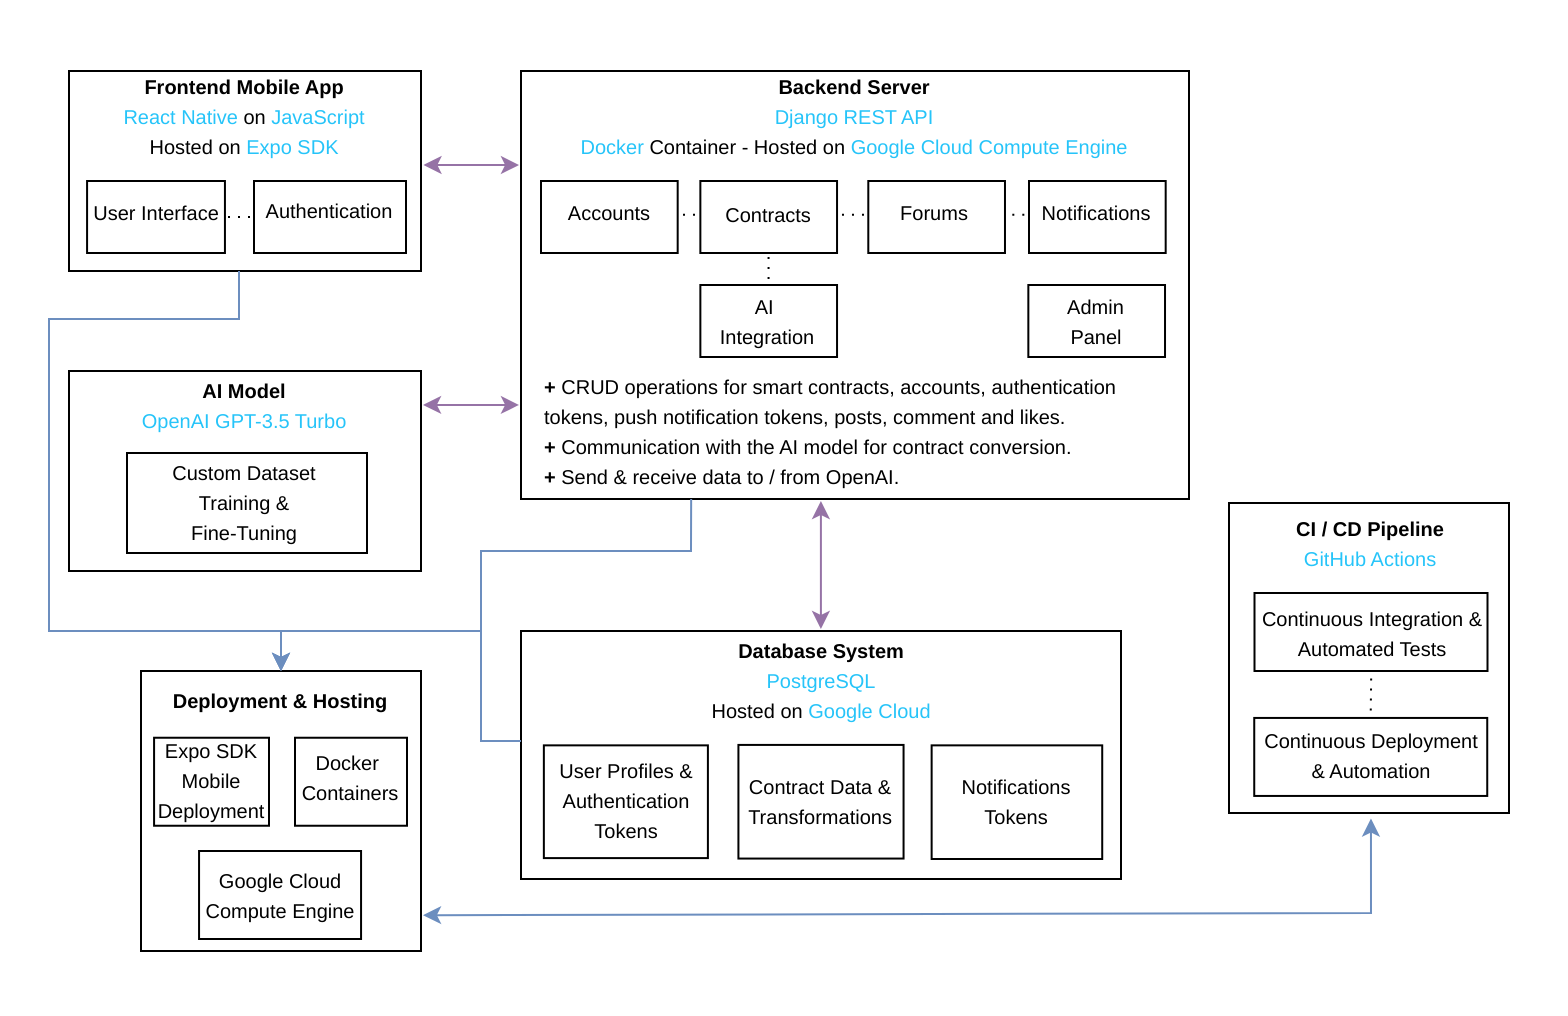
\includegraphics[width=1\linewidth]{LATEX/Appendices/Images/Software/software-diagram.png}
    \caption{Software Diagram}
    \label{fig:software-diagram}
\end{figure}

The platform will use Generative AI and smart contracts to address issues of automation and security in employment contracts. This will be achieved through fine-tuning \texttt{OpenAI's GPT-3.5 Turbo} model on a custom dataset to train it to convert legal employment contracts into smart ones. The backend server will be based on \texttt{Django Rest API} to handle data processing and interactions with the AI model. Apart from that, the mobile application interface will be built with \texttt{React Native on JavaScript}.

\section{Requirements and Objectives}

In order to successfully implement the platform, several requirements and objectives must be met. These needs can be divided into functional and non-functional categories.

\subsection{Functional Requirements}

Functional requirements specify the behaviours and features that the platform must exhibit in order to satisfy user demands and project objectives. Amongst them are:

\begin{itemize}
    \item \textbf{Contract Conversion:} The platform must be able to convert traditional employment contracts into smart contracts using the fine-tuned \texttt{GPT-3.5 Turbo} model.
    \item \textbf{AI Model Integration:} The AI model must be integrated into the backend, allowing for efficient processing of contracts.
    \item \textbf{User Authentication:} Users (employers and employees) must be able to securely create and manage their accounts.
    \item \textbf{User engagement:} The platform must provide a forum for users to interact with one another on topics related to the application's scope.
    \item \textbf{Contract Management:} Users must be able to create, view, update, and delete their smart contracts.
    \item \textbf{Performance Metrics:} The platform should support the input and management of performance metrics relevant to various job roles, which can later be expanded to automatic updates from the backend.
    \item \textbf{Salary Management:} The system must handle salary payments using \textit{USDC Coin}.
    \item \textbf{Notifications:} The platform must send notifications to users regarding contract updates, salary payments, and other relevant events.
    \item \textbf{Mobile Application:} The mobile application must provide a user-friendly interface for both iOS and Android users to interact with the platform's features.
    \item \textbf{Custom Theming:} The user interface (UI) should support dark and light modes.
    \item \textbf{Admin Panel:} The backend must include an admin panel for managing users, contracts, and system settings efficiently.
    \item \textbf{Dispute Resolution:} The platform should provide mechanisms for resolving disputes between employers and employees based on contract terms.
\end{itemize}

\subsection{Non-Functional Requirements}

Non-functional requirements verify that the platform operates efficiently and reliably. These include:

\begin{itemize}
    \item \textbf{Scalability:} The system must be able to handle an increasing number of users and contracts without performance degradation.
    \item \textbf{Security:} The platform must securely handle data, especially the one concerning financial transactions and sensitive contract details. This includes secure authentication and regular audits.
    \item \textbf{Reliability:} The platform must be highly reliable, with minimal downtime, to ensure users can access and manage contracts whenever needed.
    \item \textbf{Performance:} The system must provide quick response times for user interactions, contract processing, and AI model predictions.
    \item \textbf{Usability:} The mobile application interface must be intuitive to provide a positive user experience.
    \item \textbf{Compliance:} The platform must comply with relevant regulations regarding employment contracts and data protection.
    \item \textbf{Maintainability:} The codebase should be modular and well-documented, allowing for easy maintenance and future updates.
    \item \textbf{Portability:} The system should be deployed across various environments through cloud services with minimal configuration changes.
\end{itemize}

\section{Conceptual Development and Methodological Shifts}

\subsection{Rationale Behind Architectural Choices}

The decisions on architecture were based on the needs for efficiency, scalability, and robustness. Every component of the platform has been picked to maximise the output of the functionality, simultaneously providing a good user experience.

\subsection{AI Model Selection}

\begin{itemize}
    \item \textbf{Hugging Face Models:} Selecting the appropriate AI model for fine-tuning was one of the most important early decisions to make. Initially, it was planned to take a \texttt{seq2seq} transformer model from \texttt{HuggingFace} and train it through \texttt{PyTorch} framework. However, upon further investigation it became clear that the vast majority of available models there were based on the \textit{GPT} architecture ranging from version \textit{2.0} to \textit{3.0} \cite{GerstmayrEtAl2024, Campesato2023}. Although these variations are quite effective, they are still much worse than more modern ones. Moreover, \textit{HuggingFace} itself suffers from multiple limitations, including the challenge of context-dependent model selection \cite{NarayananEtAl2023}. With over 262,000 models available, users face the daunting task of choosing the optimal model for specific workflows or data domains, complicated by the wide variety of model architectures, sizes, and training paradigms \cite{Jones2024, NarayananEtAl2023}. Additionally, different models exhibit variable performance across tasks and datasets, meaning that a model excelling in one area may not be suitable for another, necessitating extensive testing and customisation \cite{NarayananEtAl2023, Campesato2023}. Yet, for the sake of exploring possible options, it was attempted to fine-tune two models from the platform: \textit{Salesforce/codegen-350M-multi} and \textit{EleutherAI/gpt-neo-125m}. Nonetheless, no significant results have been achieved, as the models were not generalising properly. It was most likely because of the architecture limitations \cite{LucianoEtAl2020}, such as a lack of contextual awareness, inability to fully understand complex contractual terms, and challenges in generating syntactically correct \textit{Solidity} code. To be more precise, these models struggled the most with the translation of elements like wallet addresses and transactional clauses. No mistakes can be tolerated here since if the model interprets an address wrongly, this would result in financial losses. Consequently, this led to the exploration of other models unrelated to \textit{HuggingFace}, bringing us to \textit{OpenAI}. 
    \item \textbf{OpenAI Models:} While investigating \textit{OpenAI} further, it became apparent that they allow for fine-tuning one of the latest models, \texttt{GPT-3.5 Turbo}. The process simply requires the provision of custom datasets for training and validation \cite{LatifEtAl2024, OpenAIDocumentation2023}. A \textit{GPU} is not needed since the model gets trained on \textit{OpenAI's} servers \cite{ChatGPTFineTuning2024, OpenAIDocumentation2023}. Moreover, \textit{HuggingFace} models require manually writing the training algorithm. This includes tokenisation logic with appropriate padding and encoding, selecting the appropriate batch sizes, setting up warm-up steps, weight decays, and evaluation strategies \cite{NarayananEtAl2023}. The problem is, it is hard to select the best figures, and to do so, one needs a deep knowledge of how transformers work. On the contrary, \textit{OpenAI} does not require these patterns to be specified, as they pick the best options for each specific case automatically through permutations during the training process \cite{OpenAIDocumentation2023}. This has further highlighted the advantage of OpenAI's solution.
\end{itemize}

Summarising, this model was chosen because of its advanced natural language processing capabilities compared to earlier versions of that transformer, such as \textit{GPT-2.0}. The \textit{GPT-3.5 Turbo} model is financially practical, given the ratio of cost to performance. However, it is worth noting that at the time of the design phase, the \textit{GPT-4.0} model was not yet available for fine-tuning, limiting the choice to existing models. Moreover, other options from \texttt{HuggingFace} were considered and implemented; however, they neither scaled properly nor generalised effectively. This is in terms of handling large volumes of queries without degradation in response times or accuracy, making us ultimately stop on \textit{OpenAI's} solution.  
        
\subsection{Selection of Backend and Frontend Frameworks}

At the beginning of the project, it was planned to use Flask for the backend and native development for the mobile interface. Flask, a simple Python web framework, seemed like a good choice because of its simplicity. It was also considered to implement separate Android and iOS interfaces to take advantage of the platform-specific features. However, moving forward, it was realised that these choices had some drawbacks:

\begin{itemize}
    \item \textbf{Scalability Concerns with Flask:} Starting with Flask was a good idea at first, but  concerns arose regarding its scalability and ability to handle the complex data processing \cite{Ghimire2020, CopperwaiteEtAl2015} required by the AI and smart contract components efficiently as the project grew.
    \item \textbf{Duplication of Efforts in Native Development:} Developing separate native applications for \texttt{Android} and \texttt{iOS} would have meant doubled effort, increased development time, and challenges in maintaining code consistency across platforms \cite{MasielloEtAl2017}.
\end{itemize}

These findings led to a change towards Django Rest API and React Native. The rationale behind this shift was multi-faceted:

% addd citations here for hte other frameworks %
\begin{itemize}
    \item \textbf{Django Rest API:} This framework offers time-proven robustness, which arises from the large amount of existing built-in functionalities and community support \cite{HillarEtAl2018}. Apart from that, it is well-documented, secure and reliable \cite{Ghimire2020, HillarEtAl2018}. Moreover, the framework itself is relatively easy in terms of syntax, and the entry threshold is quite low compared to other popular frameworks \cite{HillarEtAl2018, EliseevaEtAl2020, Plekhanova2009, Mao2018} such as \texttt{Ruby on Rails} \cite{LaurentEtAl2008}, \texttt{Node.js} \cite{Mead2018} and \texttt{ASP.NET} \cite{Ragupathi2016}. Additionally, it was chosen due to personal familiarity, which would significantly speed up the implementation phase. On top of that, the admin panel provided by it simplifies data management tasks \cite{HillarEtAl2018}. Last but not least, it was decided to progress with the \texttt{Django Rest API} option since \textit{Flask} is not providing many built-in functionalities, heavily relaying on third-party libraries \cite{ChanEtAl2019}. Summarising, \textit{Flask} is more suitable for lightweight web applications \cite{ChanEtAl2019}. 
    \item \textbf{React Native:} This framework was chosen primarily due to its ability to maintain one codebase for \texttt{iOS} and \texttt{Android} platforms, significantly reducing the development time \cite{MasielloEtAl2017}. Research shows that users tend to prefer mobile applications over websites for tasks that require regular interactions \cite{TurnerMcGrievyEtAl2016, TupikovskajaOmovieEtAl2015, AlmarashdehEtAL2019, Warcholinski2024}. Although it is worth admitting that the researches presented are more focused on mobile applications developed for healthcare and sales, they still indicate that user engagement with these is slightly better than with websites. Furthermore, the choice was also driven by the desire to learn this framework, as it is widely adopted nowadays. Additionally to native development, alternatives like \texttt{Flutter} have been considered. However, the large community of \texttt{React Native} and its mature ecosystem \cite{Wu2018, Boduch2017} swayed the choice towards it. Another major factor was that \texttt{React Native} allows for integration with native components \cite{Boduch2017}, which is extremely important in our case as we need secure storage for smart contracts when they are passed to users. Lastly, as \texttt{React Native} is almost identical to \texttt{React} \cite{Boduch2017}, this means that as soon as the mobile application is developed, the platform can easily be extend by creating a website. And due to the similarities between these frameworks, learning one would allow for easier adaptation to the other.
\end{itemize}

These technologies were integrated to ensure the platform meets the current demands and adapts for future expansions. The choice of each component provides a robust foundation for the platform’s success if implemented properly.

\subsection{Database System Selection}

\texttt{PostgreSQL} was chosen as the main database for the platform because it met several important needs for the project. The data being managed includes authentication and notification tokens, account details, and extensive text content for legal employment contracts and their smart counterparts. This required a database that could handle a lot of information quickly, scale properly, and manage text effectively.

\begin{itemize}
    \item One of the reasons \texttt{PostgreSQL} is so great at handling complex data with large volumes of text is its advanced indexing and full-text search features, making it an ideal solution for applications that need fast search and retrieval of large amounts of text data \cite{WorsleyEtAl2002}. Furthermore, it is overwhelmingly vital to keep up with the accuracy of transactional data while dealing with legal and contractual obligations. \textit{PostgreSQL} fully complies with the principles of Atomicity, Consistency, Isolation, and Durability \cite{JubaEtAl2015}. It thus provides a guarantee for the reliable processing of all transactions. Lastly, the ecosystem and community of \textit{PostgreSQL} are huge. Hence, there is a great volume of plugins, tools, and support \cite{FotacheEtAl2013} which will ease management, integration, and troubleshooting. 
    \item \textit{PostgreSQL} has the ability to not only function as a relational but also as a \texttt{NoSQL} database \cite{TruskowskiEtAl2020}. In contrast, many \textit{NoSQL} databases are highly scalable but may compromise on transactional integrity. \textit{PostgreSQL}, however, balances both. It can manage a large increase in data volume and many users at the same time with little drop in performance \cite{DouglasEtAl2003, TruskowskiEtAl2020, FotacheEtAl2013}. This is important for a platform that will grow and handle more employment contracts. Furthermore, \textit{NoSQL} databases can handle various data types, such as unstructured text, multimedia files, and large data blobs. Their schema-less design allows flexibility for changes in data structure \cite{FotacheEtAl2013}, which is helpful for applications with dynamic data forms. However, for this application, the main data types are structured text strings and numerical values for user and contract data. The relational database model of \textit{PostgreSQL} is more suitable for this purpose. It offers structured query capabilities and strong transaction support \cite{WorsleyEtAl2002, TruskowskiEtAl2020, FotacheEtAl2013}, which are crucial for consistent and reliable management of all application data interactions.
    \item Comparing it with \texttt{MS SQL Server}, we can conclude that the latter is a powerful database, but its licensing and operational costs are higher compared to \textit{PostgreSQL}, since it is open-source \cite{TruskowskiEtAl2020, FotacheEtAl2013}. 
\end{itemize}

In summary, \textit{PostgreSQL} was chosen for its powerful data handling abilities, especially for complex and large text data. Its adherence to \textit{ACID} compliance ensures transactional integrity. Additionally, \textit{PostgreSQL} is cost-effective and flexible, making it a perfect fit for the project's long-term goals and scalability needs.

\subsection{Smart Contracts: Initial Idea}

The initial idea was to utilise an AI model for the purpose of converting legal employment contracts into smart ones, specifically varying based on the job role.

\begin{itemize}
    \item It was planned to train the AI model to incorporate precise job metrics for various professions at the time of translation. 
    \item For professions related to computer science, quality metrics such as the quantity and quality of commits, as well as adherence to deadlines, would have been considered. For simpler roles, such as waiter or barista, metrics would have included location tracking during work hours and sales volume from an employer's company Customer Relationship Management (CRM) database. Similarly, for salespeople, smart contracts would automatically get data on sales achievements from a CRM and use it in the contract. For teachers and lecturers, performance indicators would include the number of lectures given and student feedback. 
    \item Furthermore, to expand on these ideas, other jobs might use metrics like project completion rates for construction workers, resolution success rates for customer service roles, and adherence to treatment plans for healthcare professionals. 
\end{itemize}  

However, as the project developed, several important realisations came up.

\begin{itemize}
    \item The variety of job roles meant that each job needed its own specific metrics for performance evaluation. This created a very complex system for integrating and verifying these metrics. The main challenge was where these metrics came from — usually the CRM systems of the hiring companies. CRM systems are often very different in how they are set up and organised, which made the integration process much harder. For similar job roles, metrics might have different names in different systems, like salesAchievedEmployeeXYZ versus salesEmployeeXYZ.
    \item Addressing these challenges would require creating an AI that can understand and script data retrieval from different CRM databases. This is a very tough technical task. Questions came up about the type of data needed. Would it be just the schema of the CRM database, or would it need more detailed data sets that include real-time performance metrics?
    \item Given the wide range of potential job scenarios, the initial idea, while promising, turned out to be almost impossible to execute. It was more like a PhD-level research project than a bachelor's thesis. It needed a lot of development resources and more advanced AI capabilities than were possible within the given time and available resources.
\end{itemize}

This realisation led to refocusing the scope of the project towards developing a more generalised smart contract framework. It won't be as customised to each job's specific metrics, but it will still greatly improve transparency, security, and reliability in employment management.

\subsection{Refocusing the Scope of Smart Contracts}

The focus was shifted towards training a simpler AI model capable of producing more general smart contracts, concentrating on the most important functionalities of the system. This change aims to provide both employers and employees with trust in the system to follow through on their contract obligations without any issues.

\subsection{Smart Contracts Design}

\begin{itemize}
    \item The intention is to handle salaries using USDC Coin, a stable cryptocurrency known for its reliability coming from the fact it is backed by US dollars. This choice helps reduce the risks linked to cryptocurrency price fluctuations, ensuring that salary payments remain steady. USDC was chosen over other stablecoins like USDT because it is considered the safest option, as the developers of the coin regularly perform open audits \cite{LyonsEtAl2023, VediaEtAl2023}.
    \item Once a contract is deployed, its internal state cannot be changed unless explicitly specified in the original code. Thus, it was decided to add an external modifier that allows interaction with the contract post-deployment by the backend. This modifier is extremely important because essentially what it does is that it shifts the responsibility of tracking job performance metrics from the smart contract itself to the backend system. This is a more appropriate design choice since directly performing heavy computations in smart contracts can be financially impractical. This approach lets us focus on developing an AI model that can create generalised smart contracts for managing financial interactions between employers and employees, ensuring security for everyone involved. However, since the process of implementing job performance metrics counting by the backend is overly complex and could potentially take longer than expected, it might be postponed to a later stage.
    \item The contract will include wallet addresses of the employers and employees. This is to ensure that all transactions, whether salary payments or dispute resolutions, are executed between the correct parties.
    \item The smart contract will include features to manage the employment period. It will be possible to set start and end dates, keep track of the last salary payment date, and handle contract extensions or terminations through public functions triggered by the backend using the authorised modifier. This flexibility allows the contract to adjust to real-world employment situations.
    \item Initially, the contract will allow for basic input regarding performance scores and thresholds by the authroised app, e.g., the backend. In the future, these metrics are planned to be automatically updated by the backend using actual job performance data. 
    \item Several functions will be implemented to automate salary transfers, bonuses, and job terminations based on data sent to the smart contract from the backend. These functions will operate automatically to ensure that financial transactions, like paying salaries and bonuses, happen promptly.
\end{itemize}

A more in-depth implementation of this design will be discussed during the implementation phase in the next chapter. The decision to prioritise these basic elements was influenced by practical considerations such as feasibility and resource availability, given the complexities and the need for a dependable, tamper-proof system. This focused approach aims to establish a strong foundation for secure and efficient employment management using blockchain technology. It also lays the groundwork for future improvements that could include advanced data integration and performance metric calculations.

\section{Integration Strategy}

The integration strategy of the platform involves the following key components:

\begin{itemize}
    \item \textbf{AI Model Integration:} The trained AI model is hosted on \texttt{OpenAI's} servers. The backend communicates with it through the API provided by \textit{OpenAI} using a unique secret key. This allows the backend to send contract data to the trained AI model and receive back the processed output.
    \item \textbf{Backend:} Initially, it was planned to deploy the backend on the \texttt{AWS} platform, as it is one of the best available options at the moment. However, the downside of it is that the cost might be high. Hence, it was decided to proceed with \texttt{Google Cloud}, as it offers low-cost subscriptions. To implement this, the \textit{Google Compute Engine} platform will be leveraged, which is essentially a ``serverful'' host.
    \item \textbf{Database:} The backend also manages the \textit{PostgreSQL} database, which securely stores user profiles, various tokens for authentication / notifications handling, legal employment contracts, their smart contract transformations, and other pertinent data. The plan is to host it on \textit{Google Cloud Storage}, which is a reliable cloud-based storage solution.
    \item \textbf{Mobile Application:} The same problem was encountered with the frontend. Initially, it was intended to be deployed for both \textit{iOS} and \textit{Android} platforms on \textit{Apple Store} and \textit{Google Play Store} respectively. However, the fees these platforms require are too high and are justifiable for enterprise applications that generate revenue, not for academic projects. Hence, it was decided to proceed with \texttt{Expo's SDK}.
\end{itemize}
\chapter{Implementation}

\section{AI Model}

As mentioned in Chapter 3, \texttt{ChatGPT-3.5 Turbo} was chosen as the main AI model for converting legal employment contracts into Solidity code. To train it, two datasets are required: one for training and the other for validation. One problem encountered was the absence of pre-existing datasets for this specific task, as no prior attempts to address this conversion process were found in existing literature or online resources. Consequently, the only solution was to create a custom dataset manually. This dataset should include pairs of documents:  each containing a legal employment contract alongside its corresponding smart contract. To grasp the structure of these contracts, an analysis of a general-purpose smart contract developed will be done first.

\subsection{General Purpose Smart Contract}

As discussed in the previous chapter, the decision was made to delegate the counting of job performance metrics to the backend. This avoids the high costs of doing it within the smart contract. The main job of the smart contract is to securely hold funds and manage the employment contract transparently, helping employers and employees interact smoothly. Here is the implementation of a general-purpose smart contract:

\begin{lstlisting}[caption=General Purpose Smart Contract]
// SPDX-License-Identifier: MIT
pragma solidity ^0.8.0;

import "node_modules/@openzeppelin/contracts/token/ERC20/IERC20.sol"; // Interface for ERC20 tokens
import "node_modules/@openzeppelin/contracts/utils/ReentrancyGuard.sol"; // Prevent re-entrancy attacks

contract EmploymentContract is ReentrancyGuard {
    address public employer;
    address public employee = 0x2df1c51e09aecf9cacb7bc98cb1742757f163df7;
    address private authorisedApp; // Address of the authorised app to update metrics
    uint256 public salary; // Monthly salary amount in USDC
    IERC20 private usdcToken; // USDC token contract interface
    uint256 public startDate; // Converted to unix
    uint256 public terminationDate; // Converted to unix
    uint256 public lastSalaryPaidDate; // Tracks last salary payment date
    uint256 public performanceScore; // Performance score, updated by the authorised app
    uint256 public performanceThreshold;
    bool public isEmployed; // Employment status
    string public salaryType; // How often a salary payment to be initiated

    event SalaryUpdated(uint256 newSalary);
    event BonusPaid(uint256 bonusAmount);
    event EmploymentTerminated(string message);
    event DisputeResolved(string message);
    event SalaryPaid(uint256 amount);
    event PerformanceScoreUpdated(uint256 score);
    event PerformanceThresholdUpdated(uint256 threshold);
    event TerminationDateUpdated(uint256 newTerminationDate);

    modifier onlyAuthorisedApp() {
        require(msg.sender == authorisedApp, "Caller is not the authorised app");
        _;
    }

    constructor(
        address _authorisedApp,
        address _usdcTokenAddress
    ) {
        employer = msg.sender; // The address deploying the contract is the employer
        authorisedApp = _authorisedApp;
        usdcToken = IERC20(_usdcTokenAddress);
        lastSalaryPaidDate = startDate; // Initialise with start date
    }

      // Function to check contract balance (for employer's view)
    function checkContractBalance() external view returns (uint256) {
        return usdcToken.balanceOf(address(this));
    }

    // Function to deposit USDC into the contract for salary payments
    function depositSalaryFunds(uint256 _amount) external nonReentrant {
        require(msg.sender == employer, "Only the employer can deposit funds");
        usdcToken.transferFrom(msg.sender, address(this), _amount);
    }

    // Function to automatically withdraw monthly salary funds from the employer
    function monthlyFunding() external onlyAuthorisedApp nonReentrant {
        uint256 amountNeeded = salary * 3; // Ensure buffer for 3 months
        uint256 currentBalance = usdcToken.balanceOf(address(this));
        uint256 shortfall = 0;

        if (currentBalance < amountNeeded) {
            shortfall = amountNeeded - currentBalance;
            // Attempt to transfer the shortfall from the employer to the contract
            usdcToken.transferFrom(employer, address(this), shortfall);
        }
    }

    // Automatically pay salary on a monthly basis
    function autoPaySalary() external onlyAuthorisedApp nonReentrant {
        require(isEmployed, "Employment has ended");
        require(block.timestamp >= lastSalaryPaidDate + 30 days, "Salary already paid for this month");
        require(usdcToken.balanceOf(address(this)) >= salary, "Insufficient funds in contract");
        require(performanceScore >= performanceThreshold, "Performance score does not meet the required threshold. Employee is underperforming");

        lastSalaryPaidDate += 30 days; // Update last salary paid date to current month
        usdcToken.transfer(employee, salary);
        emit SalaryPaid(salary);
    }

    // Update performance score
    function updatePerformanceScore(uint256 _newScore) external onlyAuthorisedApp {
        performanceScore = _newScore;
        emit PerformanceScoreUpdated(_newScore);
    }

    function updatePerformanceThreshold(uint256 _threshold) external onlyAuthorisedApp {
        performanceThreshold = _threshold;
        emit PerformanceThresholdUpdated(_threshold);
    }

    // Extend employment termination date
    function extendTerminationDate(uint256 _newTerminationDate) external onlyAuthorisedApp {
        require(_newTerminationDate > terminationDate, "New date must be after current termination date");
        terminationDate = _newTerminationDate;
        emit TerminationDateUpdated(_newTerminationDate);
    }

    // Update salary
    function updateSalary(uint256 _newSalary) external onlyAuthorisedApp {
        salary = _newSalary;
        emit SalaryUpdated(_newSalary);
    }

    // Pay bonus
    function payBonus(uint256 _bonusAmount) external onlyAuthorisedApp nonReentrant {
        require(usdcToken.balanceOf(address(this)) >= _bonusAmount, "Insufficient funds in contract");
        usdcToken.transfer(employee, _bonusAmount);
        emit BonusPaid(_bonusAmount);
    }

    // Terminate employment with mutual agreement or trigger dispute resolution if disagreement
    function terminateEmployment(bool employeePermission, bool employerPermission, bool employerFault) external onlyAuthorisedApp {
        if (employeePermission && employerPermission) {
            // If both parties agree, terminate employment and notify
            isEmployed = false;
            emit EmploymentTerminated("Employment terminated by mutual agreement.");
        } else {
            // If there is no mutual agreement, determine who does not agree and resolve the dispute
            resolveDispute(employerFault);
        }
    }

    // Additional function to handle disputes and protect the salary buffer
    function resolveDispute(bool employerFault) external onlyAuthorisedApp {
        uint256 contractBalance = usdcToken.balanceOf(address(this));
        address recipient = employerFault ? employee : employer;
        usdcToken.transfer(recipient, contractBalance);

        isEmployed = false;

        string memory resolutionMessage = employerFault 
            ? "Employer at fault, funds transferred to employee." 
            : "Employee at fault, funds transferred to employer.";
        emit DisputeResolved(resolutionMessage);
        emit EmploymentTerminated("Employment terminated due to dispute resolution.");
    }
}
\end{lstlisting}

At the commencement of the ``EmploymentContract'', a secure foundation is established by specifying the software licence and the version of the Solidity compiler. Using the SPDX licence identifier ensures compliance with the MIT licence, which encourages open-source use and modification.

After specifying the compiler version, two important components from the \texttt{OpenZeppelin}  contracts library are imported:
\begin{itemize}
    \item \textbf{IERC20.sol}: This interface allows the contract to interact with \textit{ERC20} tokens, such as the \textit{USDC} coin used for salary disbursements.
    \item \textbf{ReentrancyGuard.sol}: This security measure prevents so-called \textit{reentrancy} attacks, a common vulnerability where external calls could be exploited.
\end{itemize}

The contract inherits from \texttt{``ReentrancyGuard''} to use its protective mechanisms across all functions. The preliminary declarations initiate the main variables and the state of the contract, creating a solid foundation for its functionalities.

Key components of the contract's initial setup include state variables, events, the constructor, and the authorised app modifier. These are used for the following purposes:
\begin{itemize}
    \item State variables define essential elements such as the employer, employee, and authorised application addresses. They also cover financial and contractual terms like salary, start dates, and termination dates.
    \item Events are used to log significant state changes in the contract, like salary updates and employment termination.
    \item The constructor initialises the contract with designated addresses for the authorised application and the \textit{USDC} token interface. This prepares the contract for future interactions.
    \item The authorised app modifier restricts interaction with the contract after deployment solely to the backend. It allows data to be passed to the smart contract by it, facilitating decision-making processes. Functions triggered by the backend handle tasks like paying salaries or resolving conflicts.
\end{itemize}

\subsubsection{Financial Management Functions}

\begin{itemize}
    \item \textbf{checkContractBalance:} This function lets the employer check the contract's current USDC balance. It provides transparency about the funds held in the contract.
    \item \textbf{depositSalaryFunds:} This function allows the employer to deposit a specified amount of \textit{USDC} into the contract for future salary payments. It ensures that only the employer can make deposits, safeguarding against unauthorised fund transfers. This function is critical for maintaining the liquidity necessary for regular salary disbursements.
    \item \textbf{monthlyFunding:} Designed to automate the financial management process, this function calculates the total funds needed for the next three months of salary payments. If the current balance is insufficient, it retrieves the shortfall from the employer's account. This proactive approach ensures that the contract always has sufficient funds to meet its obligations.
    \item \textbf{autoPaySalary:} This function executes automatic salary payments on a monthly basis, provided certain conditions are met. These conditions include the employment being active, enough time passing since the last payment, having sufficient funds in the contract, and the employee meeting performance thresholds. This automates the payroll process, reducing administrative work.
    \item \textbf{payBonus:} Similar to regular salary payments, this function disburses bonuses to the employee, contingent upon the availability of sufficient funds in the contract. This helps align employee incentives with contract-based rewards.
\end{itemize}

\subsubsection{Performance and Contract Management Functions}

\begin{itemize}
    \item \textbf{updatePerformanceScore \& updatePerformanceThreshold:} These functions allow the authorised application (e.g. the backend) to update the performance score and threshold, respectively. 
    \item \textbf{extendTerminationDate:} This function provides a mechanism for extending the employment contract's termination date. This adds flexibility to the employment agreement by accommodating extensions.
    \item \textbf{updateSalary:} This function enables the authorised application to make dynamic salary adjustments. This allows the contract to adapt to new salary agreements or changes in compensation plans.
\end{itemize}

\subsubsection{Employment Termination and Dispute Resolution}

\begin{itemize}
    \item \textbf{terminateEmployment:} This function manages the early termination of employment. This can be done either by mutual agreement or through a dispute resolution process. It is crucial for managing contract endings, ensuring that terminations are handled smoothly according to the initial agreement and employee's performance metrics.
    \item \textbf{resolveDispute:} This function triggers an external dispute resolution mechanism if there is a fault by either the employer or the employee. It ensures that disputes are resolved fairly, with funds transferred according to the party at fault. 
\end{itemize}

\subsubsection{Conclusion}

These functions collectively ensure that the \texttt{``EmploymentContract''} automates regular employment processes and also provides robust mechanisms for handling disputes. This supports a stable and reliable employment framework on the blockchain.

\subsection{Training and Testing the AI Model}

After developing a general-purpose smart contract in the previous section, the next step is training the AI model. To achieve this, 100 smart contracts were created alongside their corresponding legal counterparts through fuzzing. These raw datasets can be found in the \textit{GitHub} repository under \textit{``AIModelTraining/data''}. While the \textit{Solidity} code was produced manually, generative AI was used to produce legal contracts in plain text format. These contracts include essential details like the employee's \textit{USDC} address, salary, start date, end date, and payment frequency. This dataset provided all the necessary inputs for our model, focusing on extracting key points from the legal contracts to convert them into smart contracts. While some may argue that a dataset of 100 entries is insufficient, results indicate this is more than adequate for \textit{ChatGPT-3.5 Turbo}. Each smart contract comprised approximately 200 lines of code, whereas each legal employment contract spanned about one page in a Word document. Despite the challenges of generating a large number of data entries, extensive data was not needed in view of the fact that the model trained and generalised well with the available dataset.

As previously mentioned, tasks such as counting job performance metrics, setting performance thresholds, and calling various functions within the smart contract are delegated to the backend, alleviating concerns in this area. The data was partitioned into 80\% for training and 20\% for validation. The dataset was encoded into a \texttt{JSONL} file format with the following structure:

\begin{lstlisting}[language=json, caption={Example JSON Configuration}]
{
  "messages": [
    {
      "role": "system",
      "content": "Convert the following legal employment contract into a Solidity smart contract. You shall pass back only code!"
    },
    {
      "role": "user",
      "content": "<HERE WOULD GO OUR LEGAL EMPLOYMENT CONTRACT>"
    },
    {
      "role": "assistant",
      "content": "<HERE WOULD GO OUR SOLIDITY CODE>"
    }
  ]
}
\end{lstlisting}

The structured training dataset can be accessed on the GitHub repository under \texttt{AIModelTraining/openAI LLM/contracts\_dataset\_open\_AI.jsonl}, and the validation dataset is located in the same directory under \texttt{contracts\_dataset\_validation\_open\_AI.jsonl}. The model was trained using 3 epochs, a batch size of 1, and a learning rate multiplier of 2 over 519,231 tokens across 261 training steps. Below is the chart showing the training loss.

\begin{figure}[!ht]
    \centering
    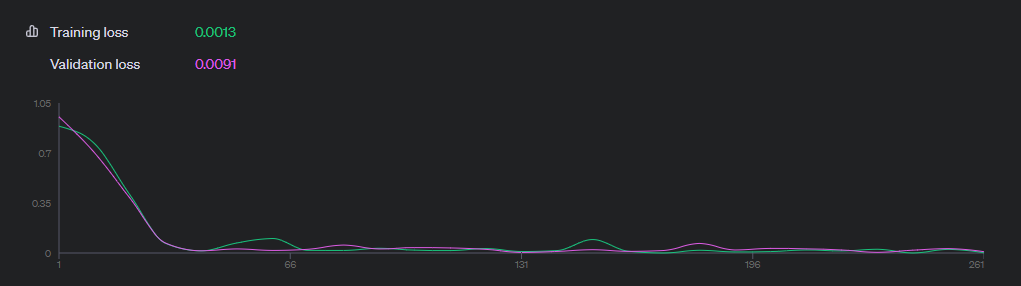
\includegraphics[width=1\textwidth]{LATEX/Appendices/Images/Software/AI Model/training_validation_loss_graph.png}
    \caption{Training Loss Graph}
    \label{fig:training_loss_graph}
\end{figure}

The training process demonstrated a significant reduction in both training and validation loss as the number of steps increased, suggesting effective learning and generalisation capabilities of the model. The detailed loss metrics, captured over 261 steps, show an initial high loss that gradually stabilises, reflecting the model’s adaptation to the complexities of translating legal contracts into Solidity code.

\begin{figure}[!ht]
    \centering
    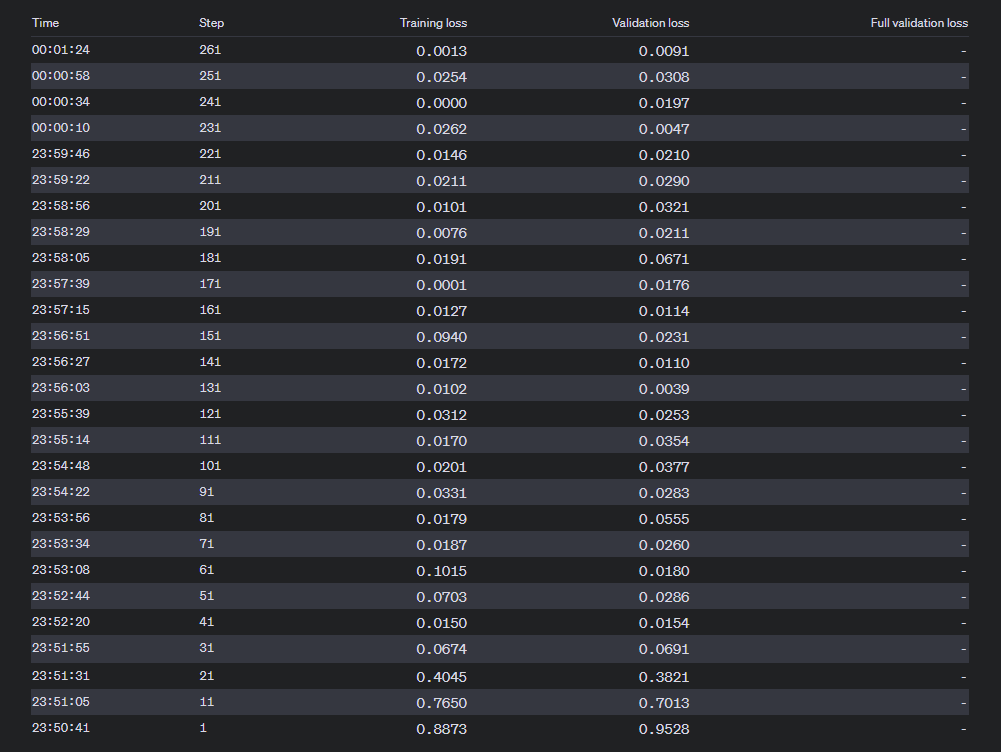
\includegraphics[width=1\textwidth]{LATEX/Appendices/Images/Software/AI Model/training_validation_loss_table.png}
    \caption{Training Loss Table}
    \label{fig:training_loss_table}
\end{figure}

\paragraph{Other Models}

As mentioned in the previous chapter, attempts were made to fine-tune two other models from \textit{HuggingFace}, but no results were achieved. The training algorithms, along with the validated datasets, can be found in the GitHub repository under \textit{``AIModelTraining/other LLMs''}.

\section{Backend}

Since the training of the AI model for contract conversions has concluded, the next step is to proceed with the backend implementation. As mentioned in the previous chapter, this will be done using \texttt{Django REST API}. 

\subsection{Project Structure}

The backend of our mobile application, referred to as \texttt{ASACBackEnd}, consists of several \textit{Django apps} that handle different functionalities of the application. In addition, the root directory contains a few files meant for  configuration and utility purposes:

\begin{itemize}
    \item \textbf{requirements.txt:} This file lists all the Python packages that the project depends on. It is used to install all necessary libraries when setting up the project in a new environment.
    \item \textbf{manage.py:} This is a command-line utility that allows interaction with the Django project. It acts as a thin wrapper around the \textit{django-admin} command-line tool for carrying out administrative tasks.
    \item \textbf{.coveragerc:} This file describes settings for code coverage reports, which help in tracking the amount of code tested as part of the quality control. 
    \item \textbf{pytest.ini:} This file configures various aspects of pytest, a framework for testing Python code. It includes settings that influence the discovery of test modules and their behaviour.
    \item \textbf{Dockerfile:} The environment and commands necessary to set up and run the application for deployment are specified in this file, which contains instructions to build a Docker image for the backend.
\end{itemize}

Apart from that, the root directory includes the \texttt{``staticfiles''} folder, which contains the following:

\begin{itemize}
    \item \textbf{admin folder:} Houses custom style-sheets, scripts, and images specifically for the Django admin interface, making it aesthetically pleasing.
    \item \textbf{rest\_framework folder:} Accommodates static files for the \textit{Django REST} Framework's browsable API. These files improve the interface's aesthetics.
\end{itemize}

Additionally, every \textit{Django app} of the project includes a directory called \texttt{``tests''} containing test files corresponding to each module written.

\subsection{Root Application}

The root application, \texttt{``ASACBackEnd''}, serves as the core of our backend architecture and includes several key configuration files that define the operational settings and the application's entry points. The naming similarity with the Django project's root follows from the adherence to Django naming conventions.

\subsubsection{Django Application Settings}

The \texttt{settings.py} includes the following key configurations and flags:
\begin{itemize}
    \item \textbf{SECRET\_KEY:} A key retrieved from the environmental variables, used for cryptographic signing and crucial for maintaining security in production.
    \item \textbf{DEBUG:} A flag retrieved from the environmental variables that turns debug mode on or off.
    \item \textbf{DATABASES:} The database configuration depends on the debug flag: it uses SQLite for non-production environments and tests, while PostgreSQL is used for production.
    \item \textbf{ALLOWED\_HOSTS:} Specifies allowed hosts, which includes development and production addresses. For development, it is \textit{``localhost''} and the local IP address of the Virtual Machine (VM) instance used during development, and for production, it is the domains \textit{``alsalibiaicontracts.co.uk''} and \textit{``www.alsalibiaicontracts.co.uk''}.
    \item \textbf{INSTALLED\_APPS:}  Specifies the apps used in the project, including custom modules.
    \item \textbf{MIDDLEWARE:} Specifies the middleware components used in the project, which process requests and responses between the client and server.
    \item \textbf{CORS\_ALLOW\_METHODS:} Specifies the HTTP / HTTPS methods allowed for Cross-Origin Resource Sharing (CORS). Only \textit{``PUT''}, \textit{``GET''}, \textit{``DELETE''}, and \textit{``POST''} are permitted, as these are the only methods needed for the project.
    \item \textbf{CORS\_ALLOWED\_ORIGINS:} Specifies the domains that are allowed to make cross-origin requests. This includes \textit{``http://localhost:8000''} for local development, and \textit{``https://www.alsalibiaicontracts.co.uk''} / \textit{``https://alsalibiaicontracts.co.uk''} for the production environment.
    \item \textbf{WSGI\_APPLICATION:} Specifies the Web Server Gateway Interface (WSGI) application path.
    \item \textbf{ASGI\_APPLICATION:} Specifies the Asynchronous Server Gateway Interface (ASGI) application path.
    \item \textbf{CHANNEL\_LAYERS:} Specifies the configuration for the channel layer, using \textit{Redis} for notifications. The configuration includes the backend and the host details, where the host is retrieved from the environment variable \textit{``REDIS\_HOST''} or defaults to \textit{``127.0.0.1''} with port \textit{6379}.
    \item \textbf{REST\_FRAMEWORK:} Configuration settings for Django REST framework.
    \item \textbf{AUTH\_USER\_MODEL:} User model for authentication, set to a custom implementation.
    \item \textbf{STATIC and MEDIA SETTINGS:} Define how static files and uploaded media are handled by the application. These are primarily used for the admin site. 
    \item \textbf{CORS SETTINGS:} Configured to allow cross-origin requests from predefined origins, essential for API interactions in a distributed environment.
    \item \textbf{Security Settings:} \textit{``USE\_X\_FORWARDED\_HOST''} enables the use of the respective header. Another flag sets the header for secure \textit{SSL} proxy. Additionally, there are settings to ensure that session and CSRF cookies are only sent over HTTPS.
\end{itemize}

\subsubsection{WSGI Configuration}

The \textit{Django} application is configured for \textit{WSGI} in the \texttt{wsgi.py} file. With the following in place, a web server is enabled to communicate and consequently handle web requests and responses.

\subsubsection{ASGI and Channels Configuration}

An instance of the \textit{ASGI} application is set up to receive \texttt{asynchronous} \textit{HTTP} and \textit{WebSocket} protocols in the \texttt{asgi.py} file. This is important for real-time features like notifications and live updates for the forums.

\subsubsection{URL Routing}

\texttt{urls.py} file manages URL patterns across the entire application, directing requests to appropriate custom views. Additionally, it sets the URL pattern for serving static files during development.

\subsection{Accounts Application}

The \texttt{``Accounts''} module within \texttt{ASACBackEnd} handles all functionalities related to user management, including registration, authentication, and the management of authentication tokens.

\subsubsection{Admin} 

The \textit{admin.py} file facilitates administrative management by establishing a connection between the Django admin interface and the user \& token models.

\subsubsection{Apps} 

This \textit{apps.py} file defines the \texttt{Accounts} application configuration, setting up essential application properties and metadata.

\subsubsection{Models} 

The \textit{models.py} file contains the \textit{User} and \textit{AuthenticationPushToken} models. The User model extends \textit{Django's} \textit{AbstractUser}, adding extra fields and validations for them. The \textit{AuthenticationPushToken} model links users to their unique push tokens.

\subsubsection{Serialisers}

The serialisers in this file handle incoming and outgoing data formats for user-related operations:

\begin{itemize}
    \item \textbf{SignUpSerialiser:} Manages user registration, ensuring data validation, password confirmation, and user creation.
    \item \textbf{UserSerialiser:} Simplifies user data serialisation for common user information retrieval.
    \item \textbf{AuthenticationPushTokenSerialiser:} Manages the creation and upkeep of user tokens for authentication..
\end{itemize}

\subsubsection{URL Configuration}

The URL configuration for the \texttt{Accounts} application defines the endpoints:

\begin{itemize}
    \item \texttt{push-token/} is linked to \texttt{AuthenticationPushTokenView}, which manages the creation and updates of authentication tokens.
    \item \texttt{validate-token/} connects to \texttt{ValidateAuthenticationTokenView}, providing a mechanism to validate user tokens.
    \item \texttt{sign-up/} is handled by \texttt{SignUpView}, facilitating new user registration.
    \item \texttt{login/} routes to \texttt{LoginView}, which supports user login functionality.
\end{itemize}

\subsubsection{Views}

The \textit{Accounts} application's views manage user interactions within the system:

\begin{itemize}
    \item \textbf{ValidateAuthenticationTokenView:} This view verifies the validity of a user's authentication token. It uses \textit{TokenAuthentication} permission to ensure that each request is made by an authenticated user. If authenticated, it returns a confirmation of token validity. Otherwise, it handles exceptions, particularly \textit{AuthenticationFailed}, by returning an invalid token response, indicating the need for re-authentication.
    \item \textbf{LoginView:} Open to all users (\textit{AllowAny} permission), this view manages user login. Upon receiving a username and password, it attempts to authenticate the user. In the case of success, it retrieves or creates a new authentication token for the session and optionally sends a push notification via the associated token. Incorrect credentials will return an error response, maintaining security by denying access.
    \item \textbf{SignUpView:} Also open to all users, this view manages user registration using the \textit{SignUpSerialiser}. It validates the incoming data, creates a new user record, and sets up initial authentication details. The view ensures that all data conforms to predefined security and integrity standards before creating the user record.
    \item \textbf{AuthenticationPushTokenView:} Restricted to authenticated users (\textit{IsAuthenticated} permission), this view manages the lifecycle of authentication tokens. Through \textit{POST}, \textit{GET}, and \textit{DELETE} requests, respectively, users can generate, obtain, and delete tokens. Before proceeding with any operations, the view verifies user's identity. To help with troubleshooting, it provides detailed error messages.
\end{itemize}

\subsection{Contracts Application}

The entire contract handling process, including the creation, validation, and deletion of employment and smart contracts, is handled by the \texttt{``Contracts''} module of \texttt{ASACBackEnd}. Users can generate their contracts directly through our AI model, which was fine-tuned earlier.

\subsubsection{Admin} 

To enable administrative management, the \textit{admin.py} file registers the \textit{SmartContract} model with Django's admin panel.

\subsubsection{Apps} 

This file sets up the application configuration with Django, defining it within the project's settings.

\subsubsection{Models} 

The \textit{models.py} file defines models like \textit{EmploymentContract} and \textit{SmartContract}, which include fields for managing contract details such as names, blockchain addresses, and content (the legal text of the employment contract and \textit{Solidity} code respectively), along with custom validators.

\subsubsection{Serialisers}

This file has two serialisers: \textit{EmploymentContractSerialiser} and \textit{SmartContractSerialiser}. These handle the conversion between model instances and data types suitable for rendering into JSON or validating data from POST requests, helping in creation and management of contract data.

\subsubsection{URL Configuration}

The URL configuration for the \textit{Contracts} application is designed to manage interactions related to contract operations:

\begin{itemize}
    \item \textbf{generate-contract/} links to \texttt{GenerateContractView}, which is responsible for initiating the generation of new smart contracts.
    \item \textbf{delete-contract/<str:contract\_name>/} connects to \texttt{DeleteContractView}, allowing users to delete specific contracts by name.
    \item \textbf{get-user-contracts/} routes to \texttt{FetchContractsView}, providing a list of all contracts associated with a user.
    \item \textbf{get-valid-checksum-address/<str:address>/} is managed by \texttt{CheckSumAddressView}, which validates Ethereum addresses.
\end{itemize}

\subsubsection{Validators}

Custom validators in \texttt{validators.py} improve data integrity:
\begin{itemize}
    \item \textbf{validate\_ethereum\_address:} Makes sure Ethereum addresses are correctly checksummed to prevent errors in blockchain transactions.
    \item \textbf{validate\_hexadecimal:} Confirms whether entries are valid hexadecimal values.
    \item \textbf{validate\_contract\_name:} Ensures the contract name is within the allowed character limits and uses only permitted characters.
    \item \textbf{validate\_json\_format:} Checks that the JSON format for contract content is correct. This is used for token interfaces that are passed to the smart contract.
\end{itemize}

\subsubsection{Views}

Functionalities of views defined in \texttt{views.py} are as follows:
\begin{itemize}
    \item \textbf{GenerateContractView:} Handles the \textit{POST} request to generate a new smart contract, transforming legal text into Solidity code. It verifies user input, communicates with our optimised AI model via the \textit{OpenAI API}, and stores the newly created smart contract in the database. The API key for communication is retrieved from the \textit{.env} file. Users receive notifications when their contracts are successfully generated.
    \item \textbf{DeleteContractView:} Offers users the ability to remove their contracts. After confirming the user's identity i.e. who owns the contract, it permits the contract to be deleted.
    \item \textbf{FetchContractsView:}  Allows users to retrieve a list of their contracts. It filters contracts by the authenticated user and serialises them for the response.
    \item \textbf{CheckSumAddressView:} Verifies user-provided Ethereum addresses to make sure they are accurate and suitable for blockchain transactions.
\end{itemize}

\subsection{Forums Application}

The \texttt{``Forums''} module within \texttt{ASACBackEnd} manages community interactions such as posts, comments, and likes. This application allows users to engage with each other, fostering a community environment within the app.

\subsubsection{Admin}

This file is responsible for configuring the Django admin panel to manage \textit{Post}, \textit{Comment}, and \textit{Like} models.

\subsubsection{Apps}

This file defines the \textit{Forums} app configuration, registering it within the Django project's ecosystem.

\subsubsection{Models} 

This file includes models for \textit{Post}, \textit{Comment}, and \textit{Like}. Each model is tied to the \textit{User} model from the \textit{Accounts} module, making sure all activities are user-specific.

\subsubsection{Serialisers}

The \texttt{Forums} application uses the following serialisers to handle data conversion between model instances and JSON:
\begin{itemize}
    \item \textbf{PostSerialiser:} Serialises post data, including related comments and like count. It includes methods to check if a post has been liked by the user and if the user is the author of the post.
    \item \textbf{CommentSerialiser:} Handles serialisation of comments, showing the username of the comment author.
    \item \textbf{LikeSerialiser:} Serialises like information, specifically tracking which user liked which post.
\end{itemize}

\subsubsection{URL Configuration}

The URL configuration for the \texttt{Forums} application routes user interactions concerning posts, comments, and likes:

\begin{itemize}
    \item \texttt{posts/} is routed to \texttt{PostListCreateView}, which facilitates the listing of all posts and the creation of new ones. This view makes sure users can both retrieve a list of posts and contribute new content within a single interface.
    \item \texttt{posts/<int:pk>/} connects to \texttt{PostDetailView}, which provides detailed information about a specific post. It allows users to retrieve, update, or delete a post based on its unique identifier.
    \item \texttt{posts/<int:pk>/comments/} links to \texttt{CommentCreateView}, enabling users to add comments to posts.
    \item \texttt{posts/<int:pk>/comments/list/} routes to \texttt{CommentListView}, which lists all comments associated with a specific post.
    \item \texttt{posts/<int:pk>/like/} is managed by \texttt{LikeCreateDeleteView}, allowing users to like or unlike a post.
\end{itemize}

\subsubsection{Views}

The views within the \texttt{Forums} module are designed to use \texttt{IsAuthenticatedOrReadOnly} permissions, ensuring that any modification to the data can only be done by authenticated users.

\begin{itemize}
    \item \textbf{PostListCreateView:}
    \begin{itemize}
        \item \textbf{GET:} Fetches and serialises a list of all posts. This operation is available to any user, authenticated or not, ensuring that the forum's content is accessible to the wider public.
        \item \textbf{POST:} Handles the creation of new posts. The view accepts data from authenticated users only, assigning the post authorship automatically to the logged-in user. 
    \end{itemize}

    \item \textbf{PostDetailView:}
    \begin{itemize}
        \item \textbf{GET:} Retrieves and serialises a single post identified by its primary key. Similarly to the \textit{``list''} view, this \textit{``detail''} view is accessible to both authenticated and unauthenticated users.
        \item \textbf{PUT:} Updates a specific post. This operation is strictly guarded to ensure that only the author of the post can make edits, thus preventing unauthorised users from altering content they do not own.
        \item \textbf{DELETE:} Removes the post from the database. Similar to the update operation, deletion is restricted to the post's author.
    \end{itemize}

    \item \textbf{CommentCreateView:}
    \begin{itemize}
        \item This view contributes to the addition of comments to posts. It ensures that each comment is linked to both the user making it and the post under which it is made. User authentication is mandatory, reinforcing that comments can only be created by logged-in users, thereby associating each comment with a specific user identity.
    \end{itemize}

    \item \textbf{CommentListView:}
    \begin{itemize}
        \item Provides a serialisation of all comments associated with a particular post. The comments are presented in reverse chronological order, ensuring that the newest comments are easily accessible. This view is read-only and does not require user authentication, allowing open access to comment data.
    \end{itemize}

    \item \textbf{LikeCreateDeleteView:}
    \begin{itemize}
        \item \textbf{POST:} Manages the creation or deletion of a like for a specific post based on its existence. If a like by the user does not exist, it is created; if it does, it is removed.
        \item \textbf{DELETE:} Explicitly removes a like from a post. This function is safeguarded to only allow the user who created the like to remove it.
        \item \textbf{Notification System:} When a post is liked for the first time, a notification is sent to the post's author, alerting them of the new like.
    \end{itemize}
\end{itemize}

\subsection{Notifications Application}

The \texttt{``Notifications''} module within \texttt{ASACBackEnd} manages everything related to notifications. This includes the registration and deletion of push tokens and the real-time delivery of notifications.

\subsubsection{Admin} 

This file registers the \textit{NotificationPushToken} model with the Django admin for administrative management.

\subsubsection{Apps} 

This file defines the application configuration for the \textit{Notifications} module. It specifies the name of the application and its default auto field.

\subsubsection{Consumers}

\textit{NotificationConsumer} is included in the \textit{consumers.py} file. It manages \textit{WebSocket} connections using \textit{Django Channels} for real-time asynchronous communication between the client and the server. Implementation in the \textit{NotificationConsumer} includes the following functions:

\begin{itemize}
    \item \textbf{connect:}
    \begin{itemize}
        \item Purpose: Establishes the \textit{WebSocket} connection between the client and the server.
        \item Process: When a client attempts to connect, this method is invoked. The consumer adds the connection to a group named \textit{``notification\_group''}. Groups in \textit{Django Channels} are a way to organise multiple connections, allowing messages to be sent to all of them simultaneously.
        \item \textbf{self.channel\_layer.group\_add}: The connect function calls this method to add the current channel to the specified group for broadcasting messages to all clients within it.
        \item \textbf{self.accept}: The connect function calls this method to finalise the \textit{WebSocket} connection, allowing data to be exchanged between the client and the server.
    \end{itemize}

    \item \textbf{disconnect:}
    \begin{itemize}
        \item Purpose: Handles the disconnection of a client from the server.
        \item Process: When a client disconnects, whether due to closing the mobile application or losing connection, this method removes the channel from the group, cleaning up resources and preventing further communication to a non-existent connection.
        \item \textbf{self.channel\_layer.group\_discard}: The disconnect function calls this method passing it the group and channel to remove the latter from the former.
    \end{itemize}

    \item \textbf{receive:}
    \begin{itemize}
        \item Purpose: Receives messages from \textit{WebSocket} clients.
        \item Process: When a message is received, this method processes it, confirms receipt by sending a message back to the client, and broadcasts it to all clients in the group.
        \item \textbf{self.send}: Sends a confirmation message back to the client who originated the request.
        \item \textbf{self.channel\_layer.group\_send}: Broadcasts the received message to all clients in the group.
    \end{itemize}

    \item \textbf{notification\_message:}
    \begin{itemize}
        \item Purpose: Distributes messages received from the \textit{group\_send} action.
        \item Process: This method is called when a message is broadcast to the group. It receives the event, which includes the message data, and then sends it to the client.
        \item \textbf{self.send}: Sends the final text data to the clients.
    \end{itemize}
\end{itemize}

\subsubsection{Models}

The \textit{models.py} file defines the \textit{NotificationPushToken} model. It links a unique notification token with a user and includes fields for the token string, creation timestamp, and a user foreign key.

\subsubsection{Routing}

Web socket URL patterns are defined in \textit{routing.py} to route notification-related \textit{WebSocket} connections to the appropriate consumer.

\begin{itemize}
    \item \textit{ws/notifications/} is routed to \textit{NotificationConsumer.as\_asgi()}. The use of the \textit{.as\_asgi} method dictates that the consumer is prepared to handle asynchronous gateway interface applications, suitable for real-time \textit{WebSocket} communications.
\end{itemize}

\subsubsection{Serialisers}

The serialisers in \textit{serialisers.py} allow the conversion of model instances into JSON format for API responses and vice versa, specifically \textit{NotificationPushTokenSerialiser} was implemented to manage serialisation and deserialisation of the \textit{NotificationPushToken} data. It handles token creation and updates while ensuring that the creation date is read-only.

\subsubsection{URL Configuration}

The URL configuration within the \textit{Notifications} module is outlined in the \textit{urls.py} file, which specifies the routes for managing notification tokens:

\begin{itemize}
    \item \textbf{save-token/} is connected to \textit{SaveTokenView}.
    \item \textbf{delete-token/} is linked to \textit{DeleteTokenView}.
\end{itemize}

\subsubsection{Utilities}

The \textit{utils.py} file includes a utility function called \textit{send\_push\_notification} that utilises the \textit{exponent\_server\_sdk} to send push notifications to users. It handles message creation and delivery, catching and logging any errors that occur during the process.

\subsubsection{Views}

Views in the \textit{Notifications} module handle API requests related to notification tokens:

\begin{itemize}
    \item \textbf{SaveTokenView:} Allows authenticated users to save or update their notification tokens. The view checks the validity of the data using the corresponding serialiser and saves the token if valid.
    \item \textbf{DeleteTokenView:} Permits authenticated users to delete their notification tokens.
\end{itemize}

\subsection{Database Configuration}

The database is configured as follows:

\begin{itemize}
    \item \textbf{Database Engine:} As previously outlined, \textit{PostgreSQL} was selected as the main database system for the \textit{ASACBackEnd} project because of its capabilities for complex queries and data integrity.
    \item \textbf{Database Name:} The database for the production environment is named \textit{``asacbackenddb''}.
    \item \textbf{Credentials:} Access to the database is secured with a username and password.
    \item \textbf{Host and Port:} The database is hosted locally on the deployment server with the default PostgreSQL port. With this configuration, database operations have quick access and reduced latency within the internal network.
    \item \textbf{Connection Settings:} By limiting access to trusted, secure sources, the database is configured to accept connections from specific IP addresses across the United Kingdom, hence enhancing security. This might be subject to change in the future.
    \item \textbf{Backup and Recovery:} To ensure data durability and dependability, regular backups are scheduled and broad recovery procedures are in place to manage any potential data loss.
\end{itemize}

\section{Frontend}

Having developed the backend, it is time now to shift our focus to the frontend implementation. As outlined in the design chapter, \texttt{ASACFrontEnd} utilises \texttt{React Native} with \texttt{JavaScript} to build the UI. 

\subsection{Project Structure}

The following configuration files are located in the root directory: 

\begin{itemize}
    \item \textbf{App.js:} Serves as the root component of our application. It initialises the navigation container and global providers such as authentication, theme, and keyboard handling. Additionally, it configures platform-specific intensifications and notification settings.
    \item \textbf{app.json:} Contains metadata for the application such as the name, version, and configuration specifics for iOS, Android and web. Additionally, it lists the plugins, assets, and other resources that must be included when the app is built.
    \item \textbf{babel.config.js:} Configures the Babel compiler for JavaScript with environment-specific settings for testing and production. This setup specifies how modern JavaScript features are translated into versions that are backward-compatible with older engines.
    \item \textbf{ErrorBoundary.js:} A higher-order component used to catch JavaScript errors anywhere in the child component tree, log those errors, and display a fallback UI instead of the component tree that crashed. This component was extensively used during the development phase for error tracking.
    \item \textbf{package.json:} Defines the project’s dependencies, scripts, and Jest configuration for testing.
    \item \textbf{package-lock.json:} This file is automatically generated when Node packages are installed (using npm) in the project. It serves to lock the versions of each package and its dependencies which were installed, ensuring that every npm install results in the exact same set of dependencies.
    \item \textbf{Dockerfile:} This file contains instructions to build a Docker image for the frontend, pushing it to expo servers for deployment.
\end{itemize}

The components of the project are organised into a main directory called \texttt{``app''}. Inside of it, there are several sub-directories, each handling a different part of the application's functionality:

\begin{itemize}
    \item \textbf{Components Directory:} Houses reusable components for handling authentication, managing notifications, applying consistent theming, and controlling keyboard interactions.
    \item \textbf{Navigation Directory:} Contains navigators that manage screen transitions.
    \item \textbf{Screens Directory:} Houses the individual screens of the \textit{app} alongside the \textit{functional hooks} that control them. Each screen is responsible for rendering the UI components relevant to the specific part of the application it represents.
    \item \textbf{Styles Directory:} Contains styling files that define the visual aspects of the application.
\end{itemize}

The test-related files of the project are consolidated into a primary directory named \texttt{\_\_tests\_\_}.

The project also includes a folder named \texttt{assets} in the root directory, which contains all the static files used in the application.

\subsection{Components Directory}

The \texttt{components} directory is organised to group essential utility components. It includes the following files:

\begin{enumerate}
    \item \texttt{Authentication.js}
    \item \texttt{Keyboard.js}
    \item \texttt{Notifications.js}
    \item \texttt{Theme.js}
\end{enumerate}

\subsubsection{Authentication Component}

\begin{itemize}
    \item \textbf{Context Setup:} The \texttt{AuthContext} is created to store authentication state and functions to manage it. Any component within the application can access it.
    \item \textbf{Token Validation:} \textit{validateToken} function checks the validity of the stored authentication token by making a \textit{GET} request to the backend. This is in place to make sure the user remains logged in even if the application restarts.
    \item \textbf{User Registration and Login:} Functions \textit{signUp} and \textit{login} interact with the backend to register new users or authenticate existing ones and manage the authentication token received from the backend.
    \item \textbf{Logout Functionality:} The \textit{logout} function erases the authentication token from storage, effectively logging out the user.
    \item \textbf{Animation and Alerts:} \textit{LayoutAnimation} is used to provide smooth login and logout transitions, while \textit{Alert} is used to give feedback on authentication procedures.
    \item \textbf{Error Handling:} Includes robust error handling to manage issues during authentication processes, easing troubleshooting and preventing the entire UI from crashing.
    \item \textbf{Higher-Order Component Usage:} Wraps the child components with \textit{WebSocketProvider} if the user is logged in, enabling \textit{WebSocket} connections for notifications.
\end{itemize}

\subsubsection{Keyboard Component}

The \texttt{Keyboard} component is a custom utility developed to manage keyboard interactions and visibility, created in response to issues encountered with \textit{React Native's} built-in \textit{KeyboardAvoidingView}, which at times did not provide reliable behaviour. The problem was that, for some reason, as soon as the \textit{KeyboardAvoidingView} was combined with the \textit{ScrollView}, the screens applying it did not focus on any input fields. To ensure a more consistent user experience, the \textit{Keyboard} component implements custom logic to handle keyboard events and adjust \textit{UI} elements accordingly. 

\begin{itemize}
    \item \textbf{Context Setup:} The \textit{KeyboardProvider} component utilises the \textit{React context API}, wrapping the application's component tree to make keyboard states and functionalities accessible across the entire application. This is achieved through the \textit{useKeyboard} hook.
    \item \textbf{State Management:} It maintains \textit{keyboardHeight} and \textit{isKeyboardVisible} states to provide real-time keyboard status.
    \item \textbf{Event Listeners:} The component sets up event listeners for keyboard \textit{show} and \textit{hide} actions. In order to keep the keyboard from covering input fields, it computes the keyboard height and modifies the layout when it is displayed. Conversely, when the keyboard hides, it resets adjustments to the layout.
    \item \textbf{Scroll Handling:} Its capacity to control scrolling actions in response to keyboard visibility is one of its primary characteristics. The component makes sure that when an input field is focused, it scrolls into view, avoiding being obscured by the keyboard. This is handled by using the \textit{registerScrollViewRef} and \textit{scrollResponderScrollNativeHandleToKeyboard} methods, respectively.
    \item \textbf{Layout Animation:} \textit{LayoutAnimation} is used for smooth transitions and layout changes when the keyboard shows or hides.
    \item \textbf{Clean-Up Logic:} To prevent memory leaks, the component cleans up event listeners when it unmounts or the provider is removed from the component tree.
\end{itemize}

\subsubsection{Notifications Component}

The \texttt{useWebSocket} hook manages a \textit{WebSocket} connection for real-time asynchronous notification functionality. Here is how it is set up:

\begin{itemize}
    \item Connection is initiated with \textit{WebSocket(url)}, which switches between \textit{wss://} and \textit{ws://} based on the backend's \textit{URL} schema for secure connections.
    \item \textbf{Event Listeners:}
        \begin{itemize}
            \item \textit{onopen:} Confirms the connection has been successfully opened and logs it to the console.
            \item \textit{onmessage:} Listens for incoming messages, then parses them, and finally triggers a notification using \textit{Expo's notification API}. This is in place to make sure that users receive alerts even when the application is not actively in use.
            \item \textit{onerror:} Handles any errors that occur during the web socket communication.
            \item \textit{onclose:} Records reasons for web socket disconnections.
        \end{itemize}
    \item Lastly, when the component unmounts, the hook makes certain the web socket connection is correctly terminated.
\end{itemize}

The component also handles push notifications through a series of functions designed to manage user tokens and permissions:

\begin{itemize}
    \item \textbf{savePushToken:} Gets a push token from \textit{Expo's notification service} and sends it to the backend server, where it is stored and associated with the user's account. This token allows the server to send push notifications to the right device.
    \item \textbf{deletePushToken:} Removes a user's token from the backend, stopping push notifications to that device.
    \item \textbf{requestNotificationPermission:} Before any notifications can be sent, the application must request and obtain permission from the user. This function handles this flow and checks the current permission status.
\end{itemize}

To make the web socket functionality accessible throughout the application, the \texttt{WebSocketProvider} component wraps the children in a context provider.

\subsubsection{Theme Component}

\begin{itemize}
    \item \textbf{Context Setup:} Spreads the theme state across the component hierarchy by utilising \textit{React's Context API}.
    \item \textbf{Persistent Theme Option:} The user's theme preference is stored persistently using \textit{expo-secure-store}, maintaining the preferred option across sessions.
    \item \textbf{Theme Switching:} Provides a \textit{toggleTheme} function, which allows users to switch between ``light'' and ``dark'' modes, updating the state within the context accordingly.
    \item \textbf{Dark Mode Support:} The \textit{isDarkMode} flag enables a check that components can use to determine if the dark mode is currently enabled, allowing for conditional styling.
\end{itemize}

The \texttt{ThemeProvider} attempts to retrieve the stored theme from safe storage when it first initialises. If a theme is saved, it sets this as the current one; otherwise, it defaults to \textit{``light''}. This setup is handled within a \textit{useEffect} hook to ensure it runs once when the component mounts.

\subsection{Navigation Directory}

The \texttt{navigation} directory is structured to facilitate user movement and access across different parts of the application. It includes the following files:

\begin{enumerate}
    \item \texttt{AppNavigator.js}
    \item \texttt{PreLoginStack.js}
    \item \texttt{PostLoginTabs.js}
\end{enumerate}

\subsubsection{AppNavigator Component}

The \texttt{AppNavigator} component acts as the primary navigation controller, directing the flow based on the user's authentication status.

\begin{itemize}
    \item To determine if the user is logged in, the component makes use of the \textit{AuthContext}. This context specifies which navigator to render based on a boolean \textit{isLoggedIn} state.
    \begin{itemize}
        \item \textit{AppNavigator} renders the \textit{PostLoginTabs} component if the user is authorised. Otherwise, it defaults to \textit{PreLoginStack}.
    \end{itemize}
    \item The \textit{SafeAreaProvider} wraps the navigator, guaranteeing that the user interface elements are displayed inside the secure regions of a device's display. This is needed to correctly handle the user interface on devices that have disruptions.
\end{itemize}

\subsubsection{PreLoginStack Component}

This stack navigator guides users through the initial authentication process with a structured sequence of screens. The component is comprised of the following features:

\begin{itemize}
    \item \textbf{Stack Navigator:} Utilises the \textit{createStackNavigator} from \textit{@react-navigation/stack} to arrange a series of screens. The stack includes \textit{PreLoginScreen}, which is configured as the initial route, \textit{LoginScreen}, and \textit{SignUpScreen}. This navigator is ideal for managing a sequence of screens where each new screen is placed on top of a stack and where the back action would pop the current screen off the stack to reveal the previous one.    
    \item \textbf{Screen Options:} The \textit{screenOptions} prop is set to \textit{ {\tt {\char '173}} headerShown: false {\tt {\char '175}} }, providing a cleaner user interface that maximises screen space and minimises distraction.
\end{itemize}

\subsubsection{PostLoginTabs Component}

The \texttt{PostLoginTabs} component allows users to switch easily between different sections of the app post-login. 

\begin{itemize}
    \item \textbf{Tab Navigation:} Applies a bottom tab navigator to offer a user-friendly way of switching between the app's main functionalities, such as \textit{home}, \textit{forum}, \textit{support}, and \textit{settings}. Each tab is associated with a specific stack navigator or screen, enabling modular navigation within the app. The navigator starts at the \textit{``Home''} tab, making it the first screen users see upon logging in. 
    \item \textbf{Icon Integration:} Utilises icons from \textit{Ionicons}, which dynamically change based on the focus state, indicating which tab is active.
    \item \textbf{Stack Navigators:} Incorporates multiple stack navigators for the \textit{home} and \textit{forum} tabs to manage more complex navigation paths that include multiple screens. For instance, the home tab can navigate to an editor screen, and the forum tab to a comment screen, both without leaving the tab context.
    \item \textbf{Theme Context:} Uses the \textit{ThemeContext} to adapt the styling of the navigation bar and other UI elements according to the selected theme. 
\end{itemize}

\subsection{Styles Directory}

The \texttt{styles} directory unifies the stylistic guidelines and guarantees a unified appearance across the application. The directory includes the following files:

\begin{enumerate}
    \item \texttt{ThemeStyles.js}
    \item \texttt{GloballySharedStyles.js}
    \item \texttt{LocallySharedStylesPreLoginScreens.js}
    \item \texttt{LocallySharedStylesForumScreens.js}
    \item \texttt{LocallySharedStylesHomeScreens.js}
    \item \texttt{LocallySharedStylesSettingsScreens.js}
    \item \texttt{LocallySharedStylesSupportScreens.js}
\end{enumerate}

\subsubsection{ThemeStyles Component}

The code snippet in this file defines a JavaScript object, \texttt{themeStyles}, which contains two sets of styles corresponding to the light and dark themes.

\begin{itemize}
    \item \textbf{backgroundColour, textColour, inputBackground, borderColour, containerBackground, cardBackground:} These properties control the main colour attributes of the UI components.
    \item \textbf{shadowColour, shadowOpacity:} By defining the shadows for UI elements, these attributes improve the visual contrast and distinction between components. The opacity settings are adjusted to make shadows more pronounced in the dark theme compared to the light one.
\end{itemize}

\subsubsection{GloballySharedStyles Component}

All of the application's screens make considerable use of style definitions, which are stored in the \texttt{GloballySharedStyles} component. The styles are dynamically generated based on the current theme, which is passed as a parameter through the \textit{ThemeStyles} component. The styles are defined using \textit{React Native's} \textit{StyleSheet.create} method. Important Style Categories consist of:

\begin{itemize}
    \item \textbf{Navigation and Layout:} The component defines styles for the tab bar and various containers. The tab bar style, for instance, includes customised active and inactive tint colours, background colour, and positioning to create a floating effect at the bottom of the screen. Container styles are adjusted for general use and, in certain circumstances, for particular contexts like modals and card views. They include settings for alignment, padding, and background colours.
    \item \textbf{Text and Typography:} A range of text styles are provided for different textual content across the UI, such as headers, general text, and modal text. These styles modify the font's weight, colour, and size based on the theme.
    \item \textbf{Interactive Elements:} Styles for buttons, file drop zones and input fields are included, defining dimensions, colour schemes, border characteristics, and alignment. To preserve functional clarity, extra care is taken with components such as exit buttons and activity indicators.
    \item \textbf{Visual Enhancements:} Extra styles such as shadows, separators, and positioning are added to make the UI more attractive.
\end{itemize}

\subsubsection{LocallySharedStyles Components}

The \texttt{LocallySharedStyles} components are utilised to:
\begin{itemize}
    \item Provide custom styling for particular screens within the application that require specific aesthetics not covered by global styles.
    \item Improve maintainability of style code by segregating local styles into dedicated modules. This reduces clutter in main component files.
    \item Allow each screen to independently control its visual elements without impacting other parts of the application, thereby easing more focused style adjustments.
\end{itemize}

The naming structure for the \textit{LocallySharedStyles} components follows a consistent pattern, prefixed with \textit{LocallySharedStyles} followed by the name of the specific component or screen they style, such as \textit{LocallySharedStylesHomeScreen.js} or \textit{LocallySharedStylesSupportScreen.js}. 

\subsection{Screens Directory}

The \texttt{Screens} directory is divided into two main subdirectories in order to control the user interfaces according to the status of authentication. The \texttt{PreLoginScreens} subdirectory contains:

\begin{itemize}
    \item \texttt{PreLoginScreen.js} - Provides introductory page functionalities.
    \item \texttt{LoginScreen.js} - Manages the user login interface.
    \item \texttt{SignUpScreen.js} - Handles user registration interface.
\end{itemize}

Users interact with screens arranged under the \texttt{PostLoginScreens} subdirectory after successfully logging in. This folder is further divided into four directories, each of which stands for a different functional area of the application:

\begin{enumerate}
    \item \textbf{Home:} Focuses on core functionalities such as contract creation and viewing. Files include:
    \begin{itemize}
        \item \texttt{HomeScreen.js} - The main dashboard screen for contract management.
        \item \texttt{ContractItem.js} - Displays individual contract items that are incorporated into the home screen. However, due to the frequent use of custom animations and states there, it was decided to segregate it into a separate file.
        \item \texttt{EditorScreen.js} - Provides an editor for contract viewing.
        \item \texttt{UseHomeScreen.js} - Custom hook for managing home screen states and logic.
        \item \texttt{UseEditorScreen.js} - Custom hook for editor functionalities.
    \end{itemize}
    \item \textbf{Forum:} Enables community interaction. Files include:
    \begin{itemize}
        \item \texttt{ForumScreen.js} - Main screen for forum discussions, where users can post.
        \item \texttt{CommentScreen.js} - Handles the display and management of comments for posts.
        \item \texttt{UseForumScreen.js} - Custom hook for forum screen logic.
        \item \texttt{UseCommentScreen.js} - Custom hook for comment functionalities.
    \end{itemize}
    \item \textbf{Support:} Offers support and help resources to the users. Files include:
    \begin{itemize}
        \item \texttt{SupportScreen.js} - Screen for user support and assistance.
    \end{itemize}
    \item \textbf{Settings:} Manages user preferences and application settings. Files include:
    \begin{itemize}
        \item \texttt{SettingsScreen.js} - Provides interfaces for adjusting user settings.
        \item \texttt{UseSettingsScreen.js} - Custom hook for settings management.
    \end{itemize}
\end{enumerate}

\paragraph{Additional Information}

All the UI components below will perform the functionalities discussed in this section. They are listed here once; future references may be omitted to avoid redundancy, as these code snippets are integrated into all the files described below.

\begin{itemize}
    \item The current theme is obtained from the \textit{ThemeContext}.
    \item Shared and local styles are generated based on the current theme.
    \item State variables are declared using the \textit{useState} hook.
    \item A reference for the \textit{ScrollView} component is created using \textit{useRef}.
    \item Keyboard height is managed using the \textit{useKeyboard} hook.
    \item The \textit{useFocusEffect} hook is used to register and unregister the \textit{ScrollView} reference when the component gains and loses focus.
    \item Interacting with navigation buttons is facilitated through the \textit{React's Navigation library}. The navigation prop is passed to the component, enabling it to command transitions to other screens within the application.
\end{itemize}

\subsubsection{PreLoginScreens: PreLoginScreen.js}

The \texttt{PreLoginScreen.js} uses the \textit{ImageBackground} component to make the screen more engaging. It is divided into three primary interactive sections, which include:

\begin{enumerate}
    \item \textbf{Login Button:} Directs users to the \textit{LoginScreen}.
    \item \textbf{Sign Up Button:} Leads new users to the \textit{SignUpScreen}.
    \item \textbf{About Us Button:} This button is designed to provide users with more information about the software. 
\end{enumerate}

\begin{figure}[!ht]
    \centering
    \includegraphics[width=0.43\textwidth]
    {LATEX/Appendices/Images/Software/Frontend/pre_login_screen.png}
    \label{fig:pre login screen}
\end{figure}

\subsubsection{PreLoginScreens: LoginScreen.js}

The rendering of the login screen is handled by the \texttt{LoginScreen} functional component. To control the login procedure, this component retrieves the \textit{handleLogin} method from the \textit{AuthContext}. The component returns a view hierarchy structured as follows:

\begin{itemize}
    \item A \textit{View} component that serves as the main container, with styles adjusted based on the keyboard height.
    \item A \textit{StatusBar} component. It is important to note that this is globally defined in the root component of the post-login tabs, but not in the pre-login ones. On the pre-login screen, there is a background image with dark colours that would obscure its elements if the white theme were applied.
    \item A \textit{ScrollView} component, which is referenced to manage keyboard interactions, that allows for scrolling when the content exceeds the screen height.
    \item Inside of it, there is a nested \textit{View} component that contains:
    \begin{itemize}
        \item Another \textit{View} component with a \textit{card} style, housing the \textit{TextInput} fields for username and password inputs.
        \item A \textit{TouchableOpacity} component that acts as the login button, triggering the \textit{handleLogin} function with the entered username and password when pressed.
    \end{itemize}
    \item A separator line at the bottom, with its position adjusted based on the keyboard height.
\end{itemize}

\begin{figure}[!ht]
    \centering
    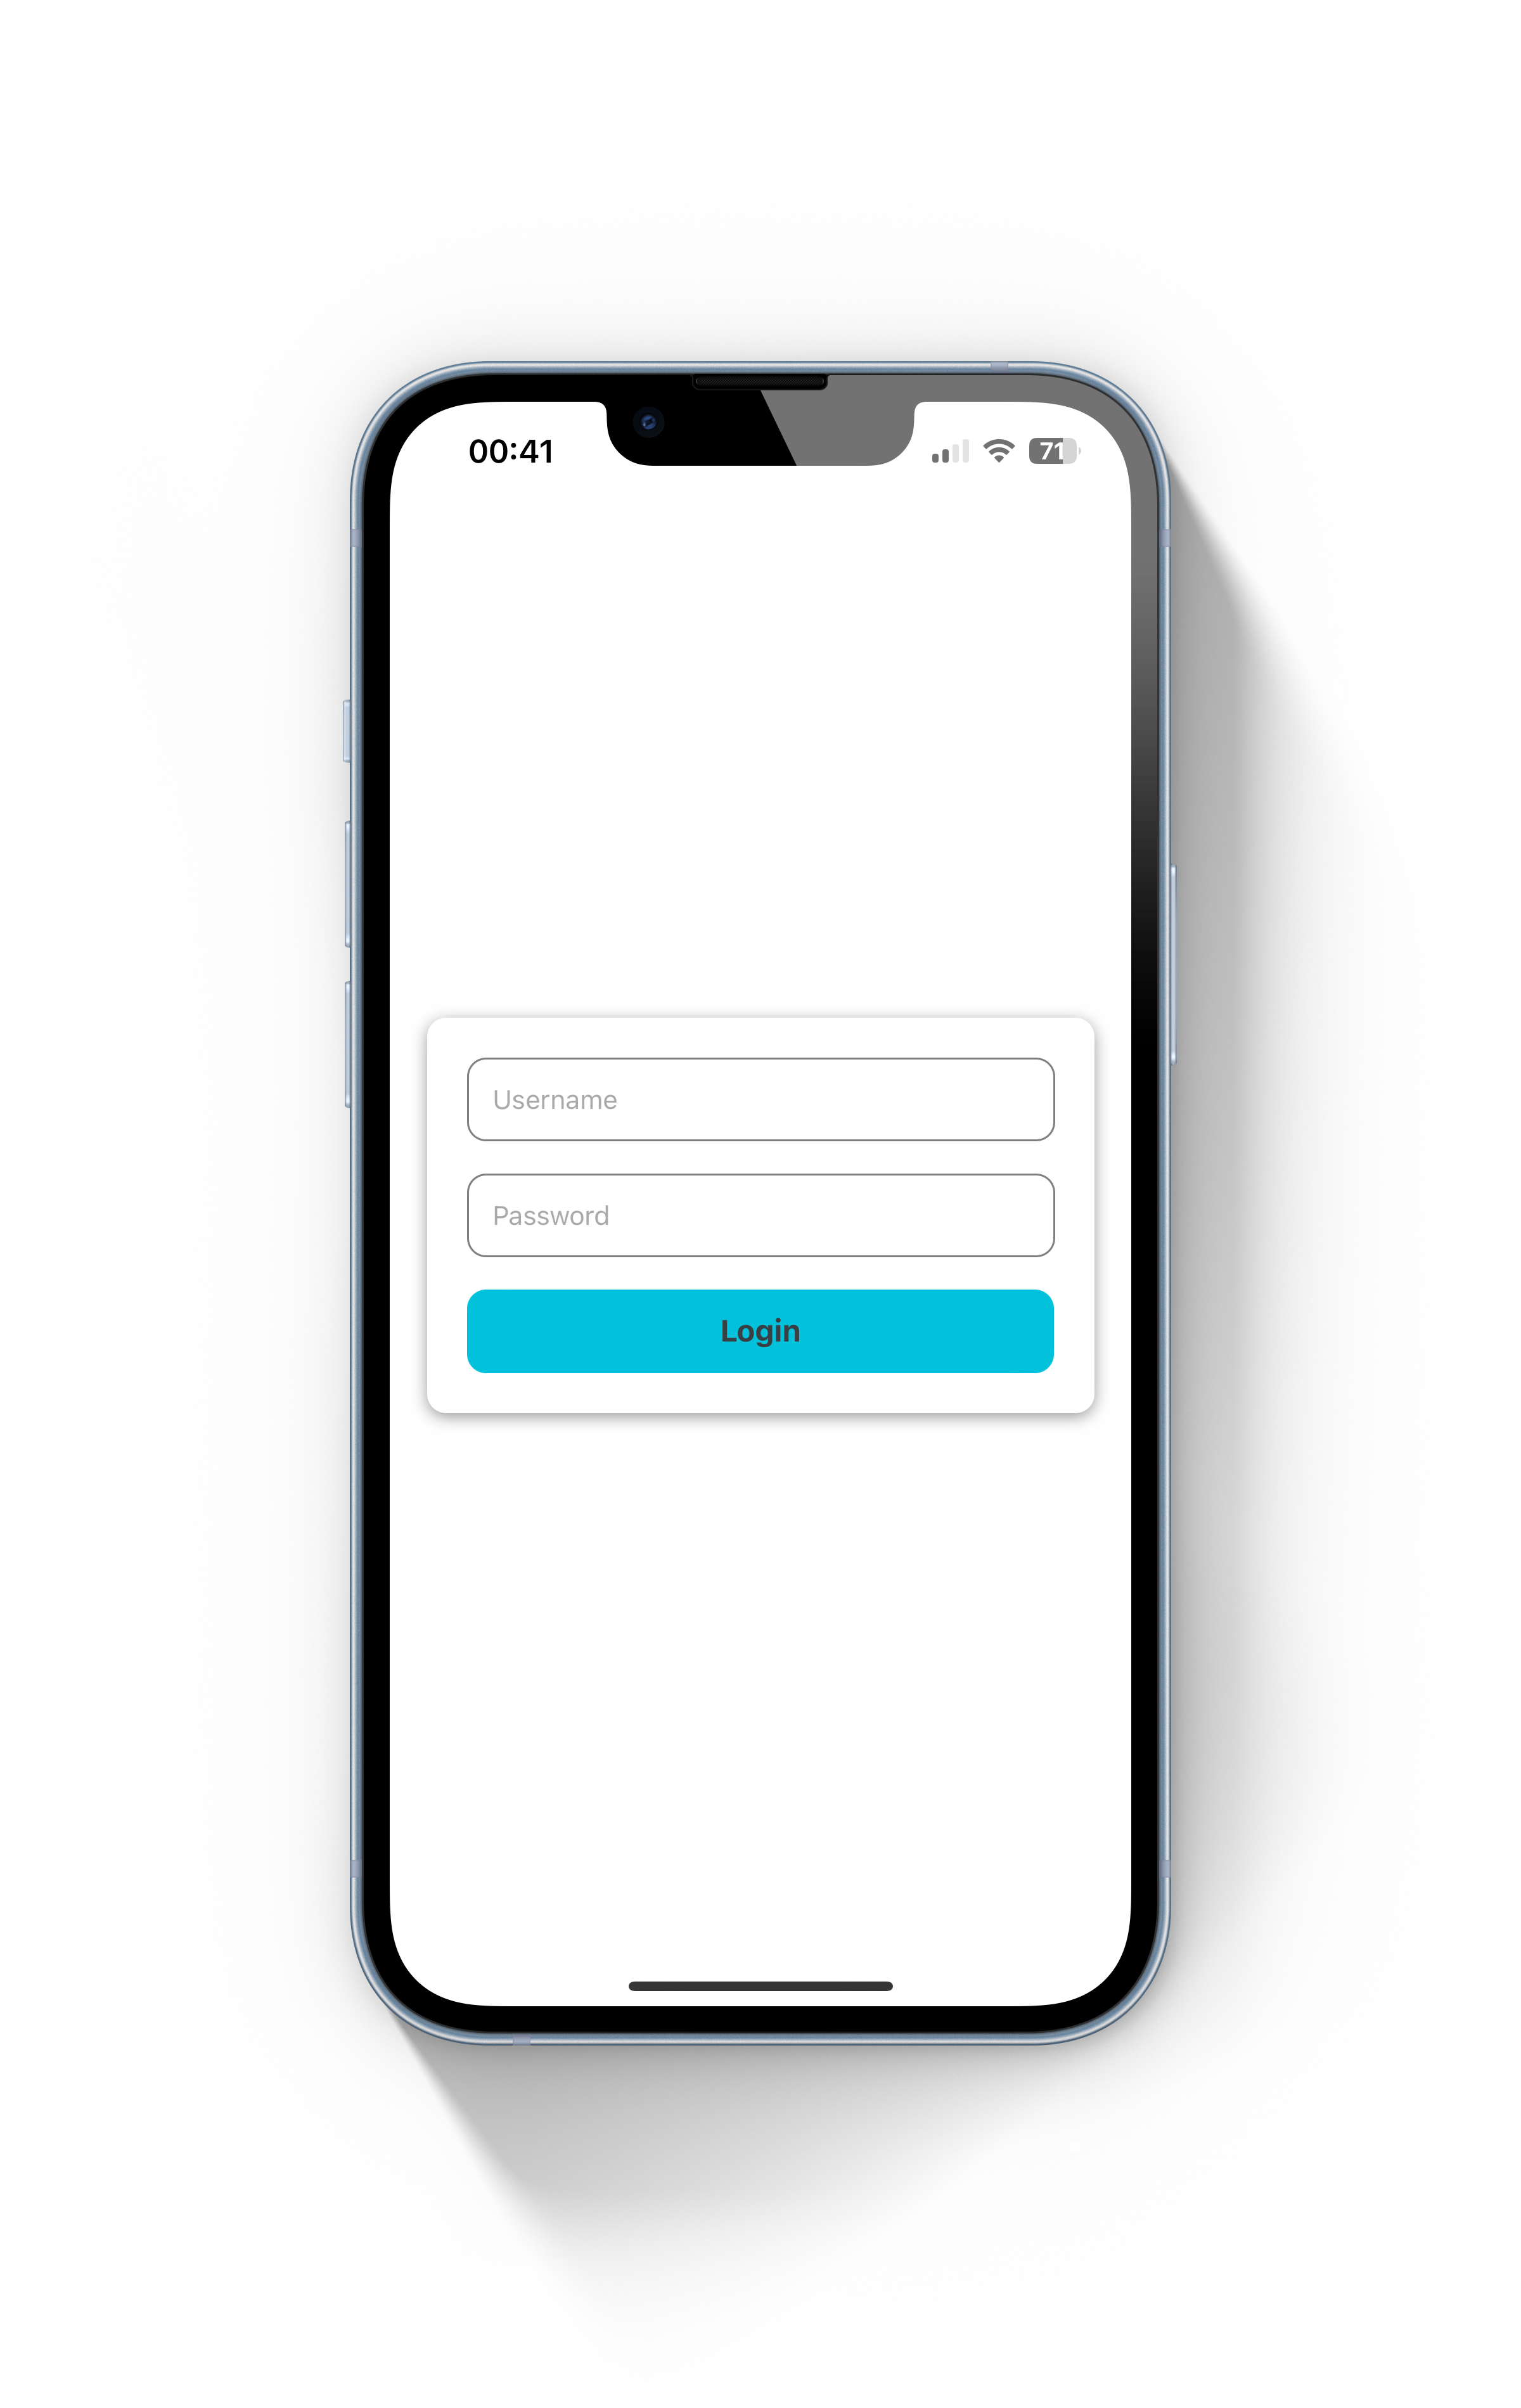
\includegraphics[width=0.43\textwidth]
    {LATEX/Appendices/Images/Software/Frontend/login_screen.png}
    \label{fig:login screen}
\end{figure}

\subsubsection{PreLoginScreens: SignUpScreen.js} 

The rendering of the sign-up screen is managed by the \texttt{SignUpScreen} functional component. Within this component, the \textit{handleSignUp} function is retrieved from the \textit{AuthContext} to manage the sign-up process. The component gives back a view hierarchy with the following structure:

\begin{itemize}
    \item A \textit{View} component that serves as the main container, with styles adjusted based on the keyboard height. 
    \item A \textit{StatusBar} component to manage the appearance of the status bar based on the current theme. It is important to note that this component is repeatedly added at the individual level of the pre-login screens since it could not be added to the root container, \textit{PreLoginStack}. The \textit{PreLoginScreen} is an exception, as the background image there is too dark, making its components invisible in case of a dark mode. Hence, this component is manually added to each individual screen, contrary to the \textit{PostLoginTabs}, where it was added once at the root component.
    \item A \textit{ScrollView} component, which is referenced to manage keyboard interactions, that allows for scrolling when the content exceeds the screen height. 
    \item Inside the \textit{ScrollView}, a nested \textit{View} component contains:
    \begin{itemize}
        \item Another \textit{View} component with a card style, housing the \textit{TextInput} fields for username, first name, last name, email, password, and password confirmation.
        \item A \textit{TouchableOpacity} component that acts as the sign-up button, triggering the \textit{handleSignUp} function with the entered details and current error state when pressed.
        \item An error icon that appears if there are validation errors, which triggers the display of a modal with error details when pressed.
    \end{itemize}
    \item The error modal, which displays a list of validation errors and allows the user to close it through the exit button.
    \item A separator line at the bottom, with its position adjusted based on the keyboard height.
\end{itemize}

\begin{figure}[!ht]
    \centering
    % Begin the first minipage for the first image
    \begin{minipage}{0.5\textwidth}
        \centering
        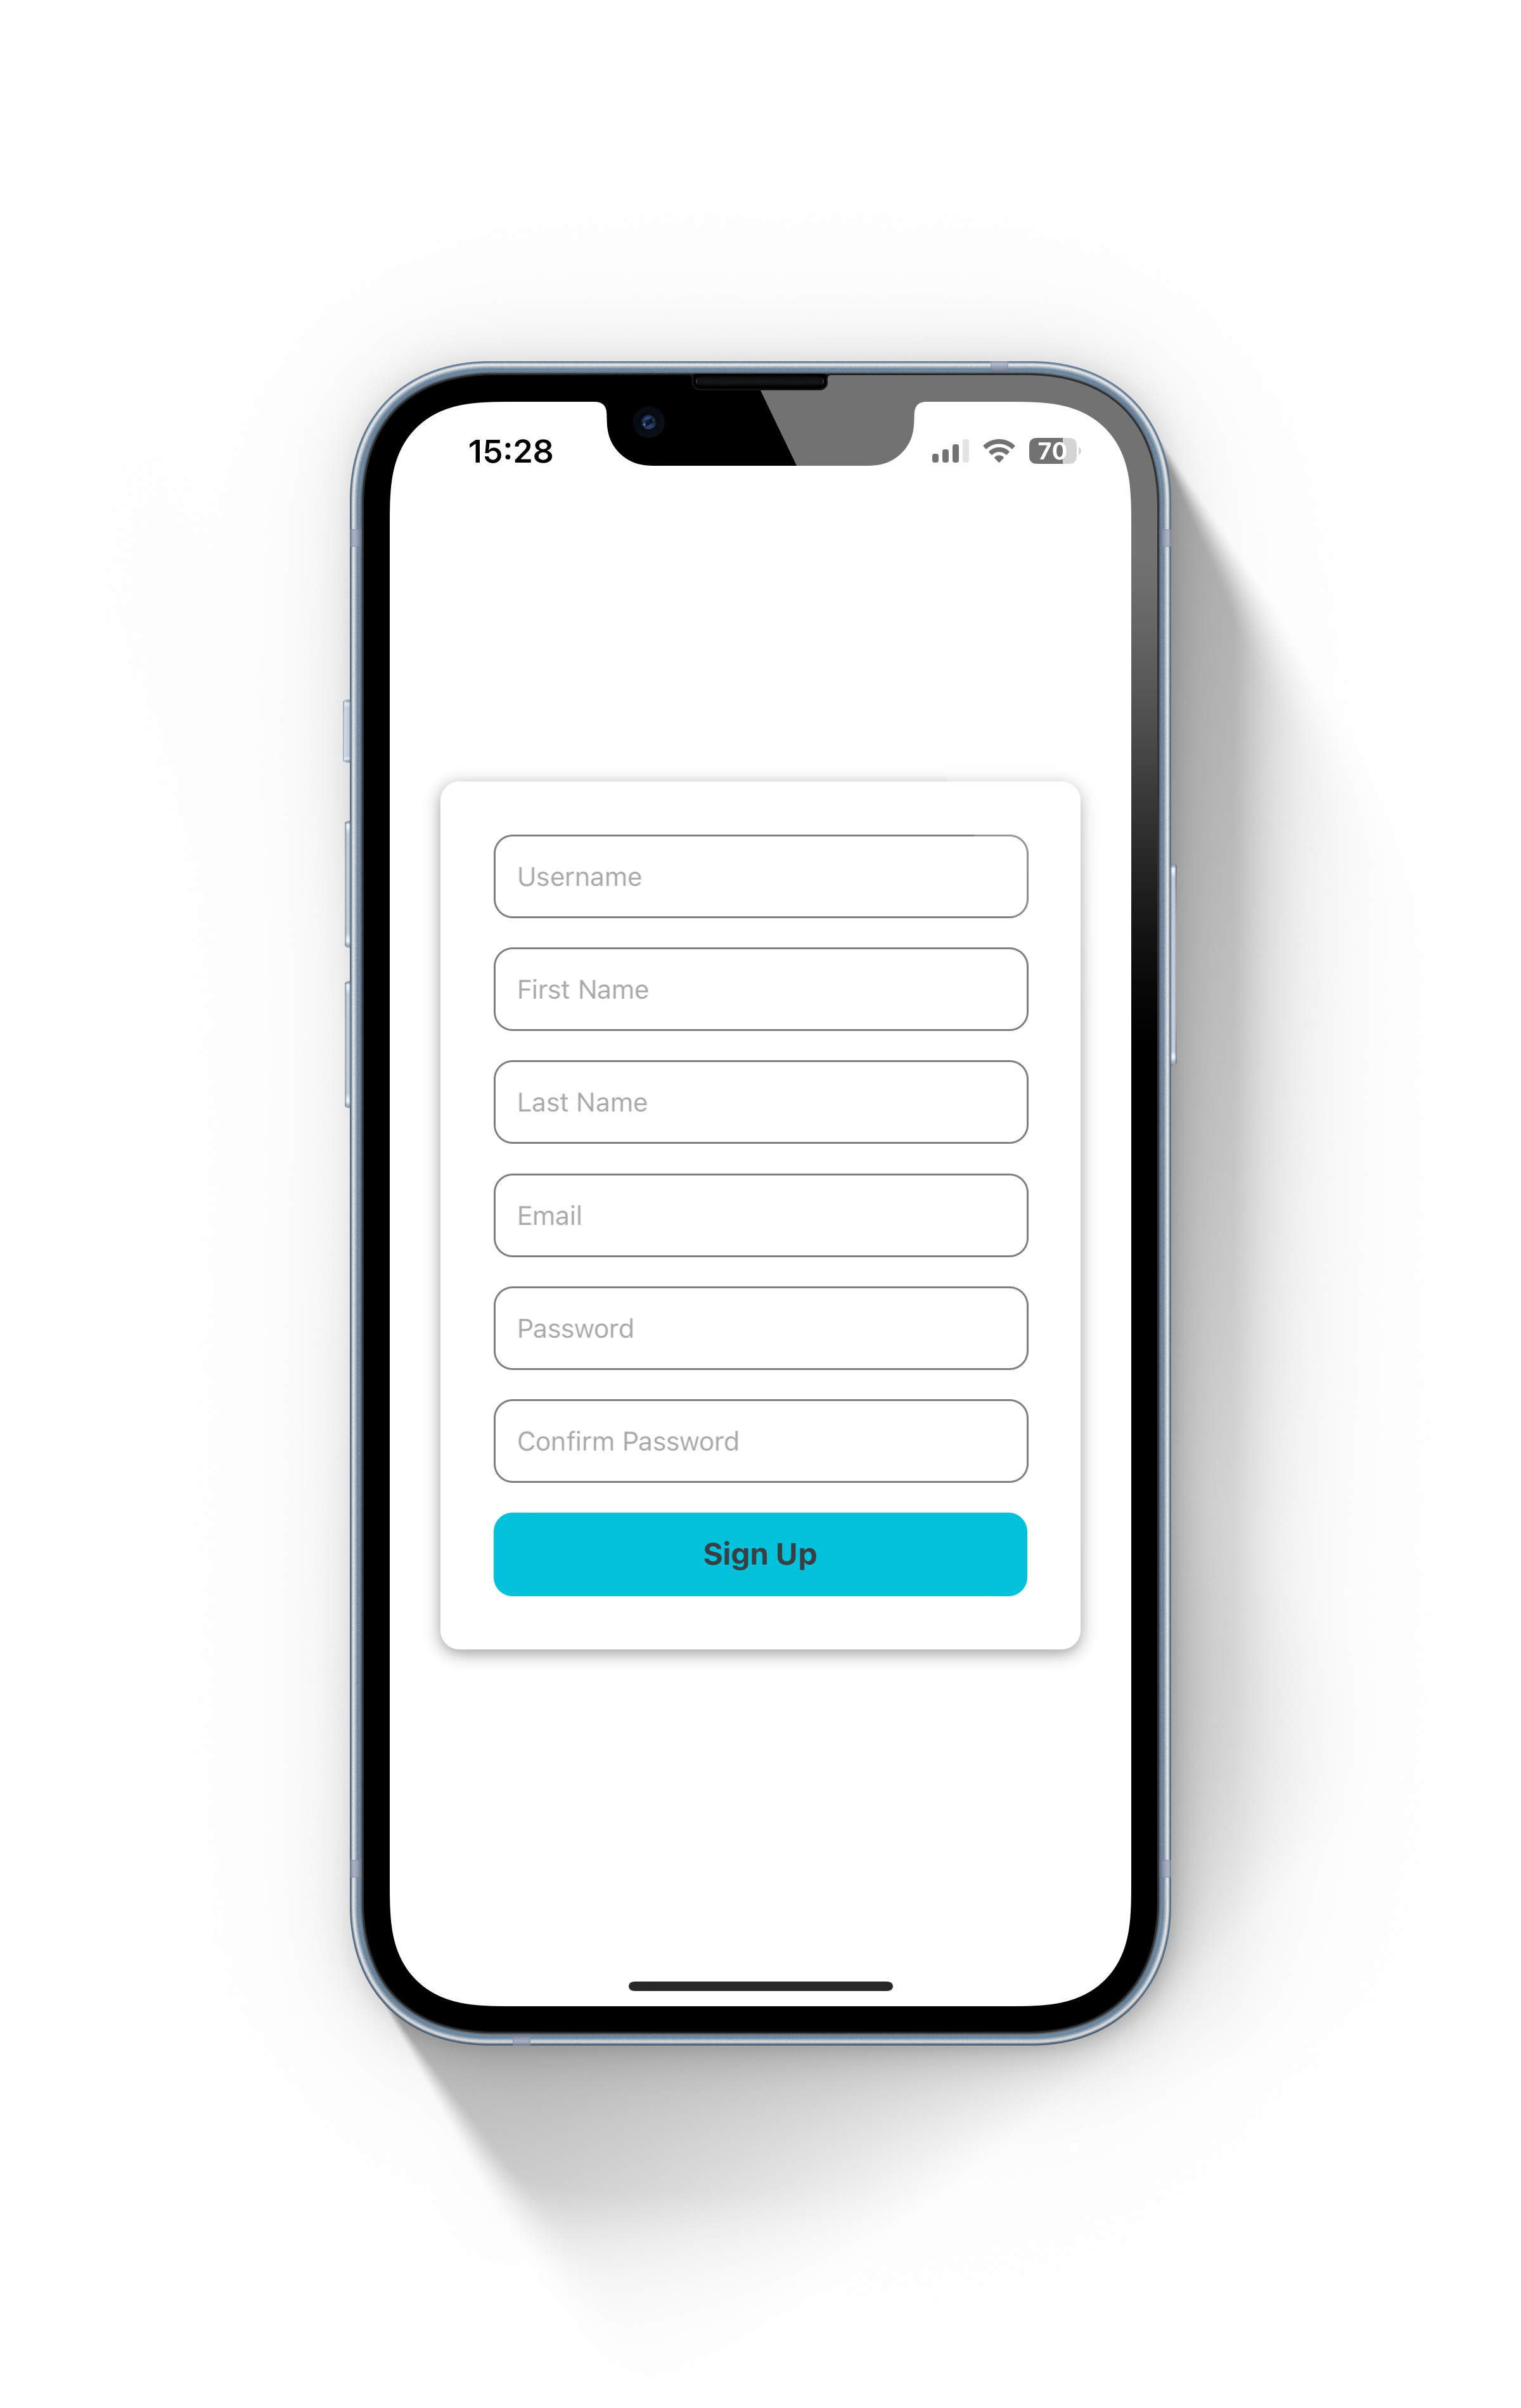
\includegraphics[scale=0.08]{LATEX/Appendices/Images/Software/Frontend/sign_up_screen_1.png}
        \label{fig:sign up screen 1}
    \end{minipage}\hfill % Insert a small horizontal space between the minipages
    % Begin the second minipage for the second image
    \begin{minipage}{0.5\textwidth}
         \centering
        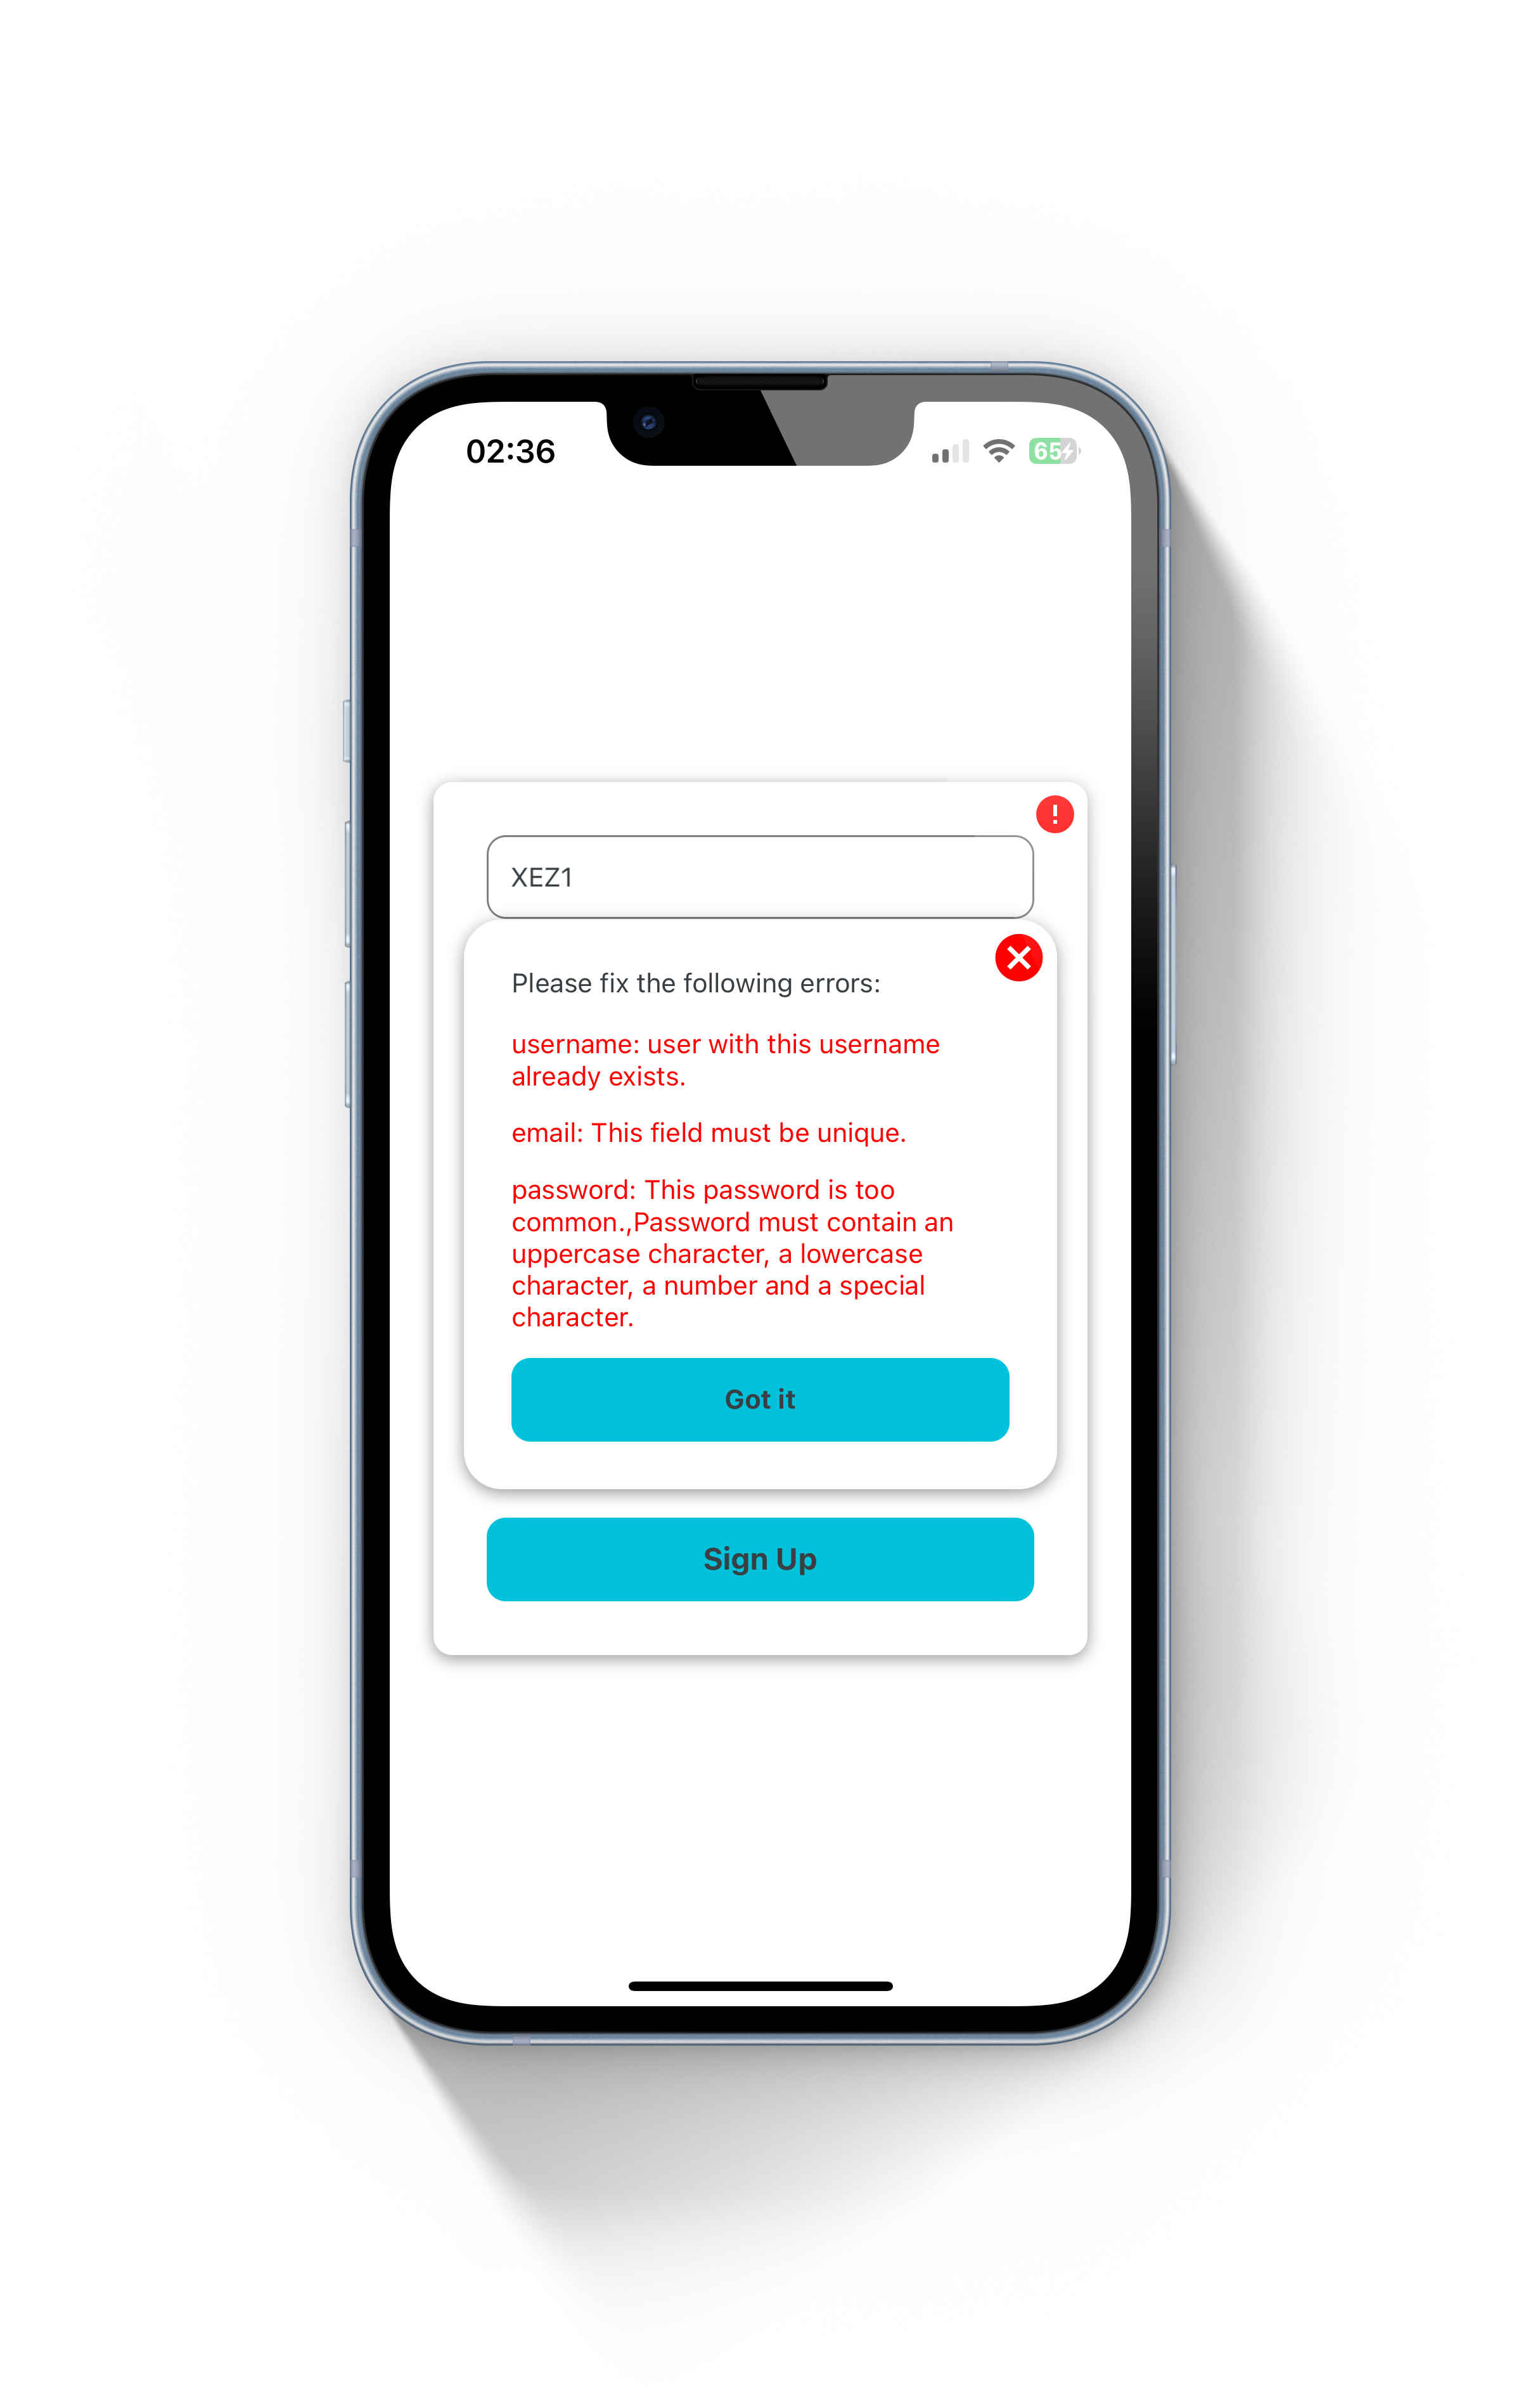
\includegraphics[scale=0.08]{LATEX/Appendices/Images/Software/Frontend/sign_up_screen_2.png}
        \label{fig:sign up screen 2}
        \end{minipage}
\end{figure}

\subsubsection{PostLoginScreens: HomeScreen.js}

The \texttt{HomeScreen} functional component handles the rendering of the home screen, which includes sections for building smart contracts, displaying saved contracts, and performing address checksum conversions. Within this component:

\begin{itemize}
    \item State variables and functions for managing contract data, user input validation, file selection, contract operations, errors, and modal visibility are retrieved from the \texttt{useHomeScreen} custom hook. This hook is responsible for the animations and all backend interactions on the home screen.
    \item The \textit{useEffect} hook is used to fetch and synchronise contracts when the component mounts.
\end{itemize}

The component returns a view hierarchy structured as follows:

\begin{itemize}
    \item A main \textit{View} container adjusted based on the keyboard height.
    \item A \textit{ScrollView} for overflow content. It is referenced to manage keyboard interactions.
    \item Inside the \textit{ScrollView}, a nested \textit{View} component contains:
    \begin{itemize}
        \item A header label for the page.
        \item A Contract creation section, styled as a card, with:
        \begin{itemize}
            \item An error icon and modal for displaying input validation errors.
            \item A card header for the contract creation section.
            \item A \textit{TouchableOpacity} component serving as a drop zone for file uploads.
            \item Multiple \textit{TextInput} components for entering contract details.
            \item A \textit{TouchableOpacity} component acting as the "Create Contract" button.
        \end{itemize}
        \item A card section for displaying the user's saved contracts, which includes:
        \begin{itemize}
            \item A card header for the saved contracts section.
            \item A list of \textit{ContractItem} components for each saved contract.
            \item A message in a visually appealing box indicating if there are no saved contracts.
        \end{itemize}
        \item A card section for address checksum conversion, which includes:
        \begin{itemize}
            \item A card header for the address checksum conversion section.
            \item A \textit{TextInput} component for entering the token address.
            \item A \textit{TouchableOpacity} component acting as the "Validate Address" button.
            \item A modal for displaying the validated address and providing options to copy or close the modal.
        \end{itemize}
        \item A footer section with copyright information.
    \end{itemize}
    \item A separator line at the bottom, with its position adjusted based on the keyboard height.
\end{itemize}

\begin{figure}[!ht]
    \centering
    % Begin the first minipage for the first image
    \begin{minipage}{0.5\textwidth}
        \centering
        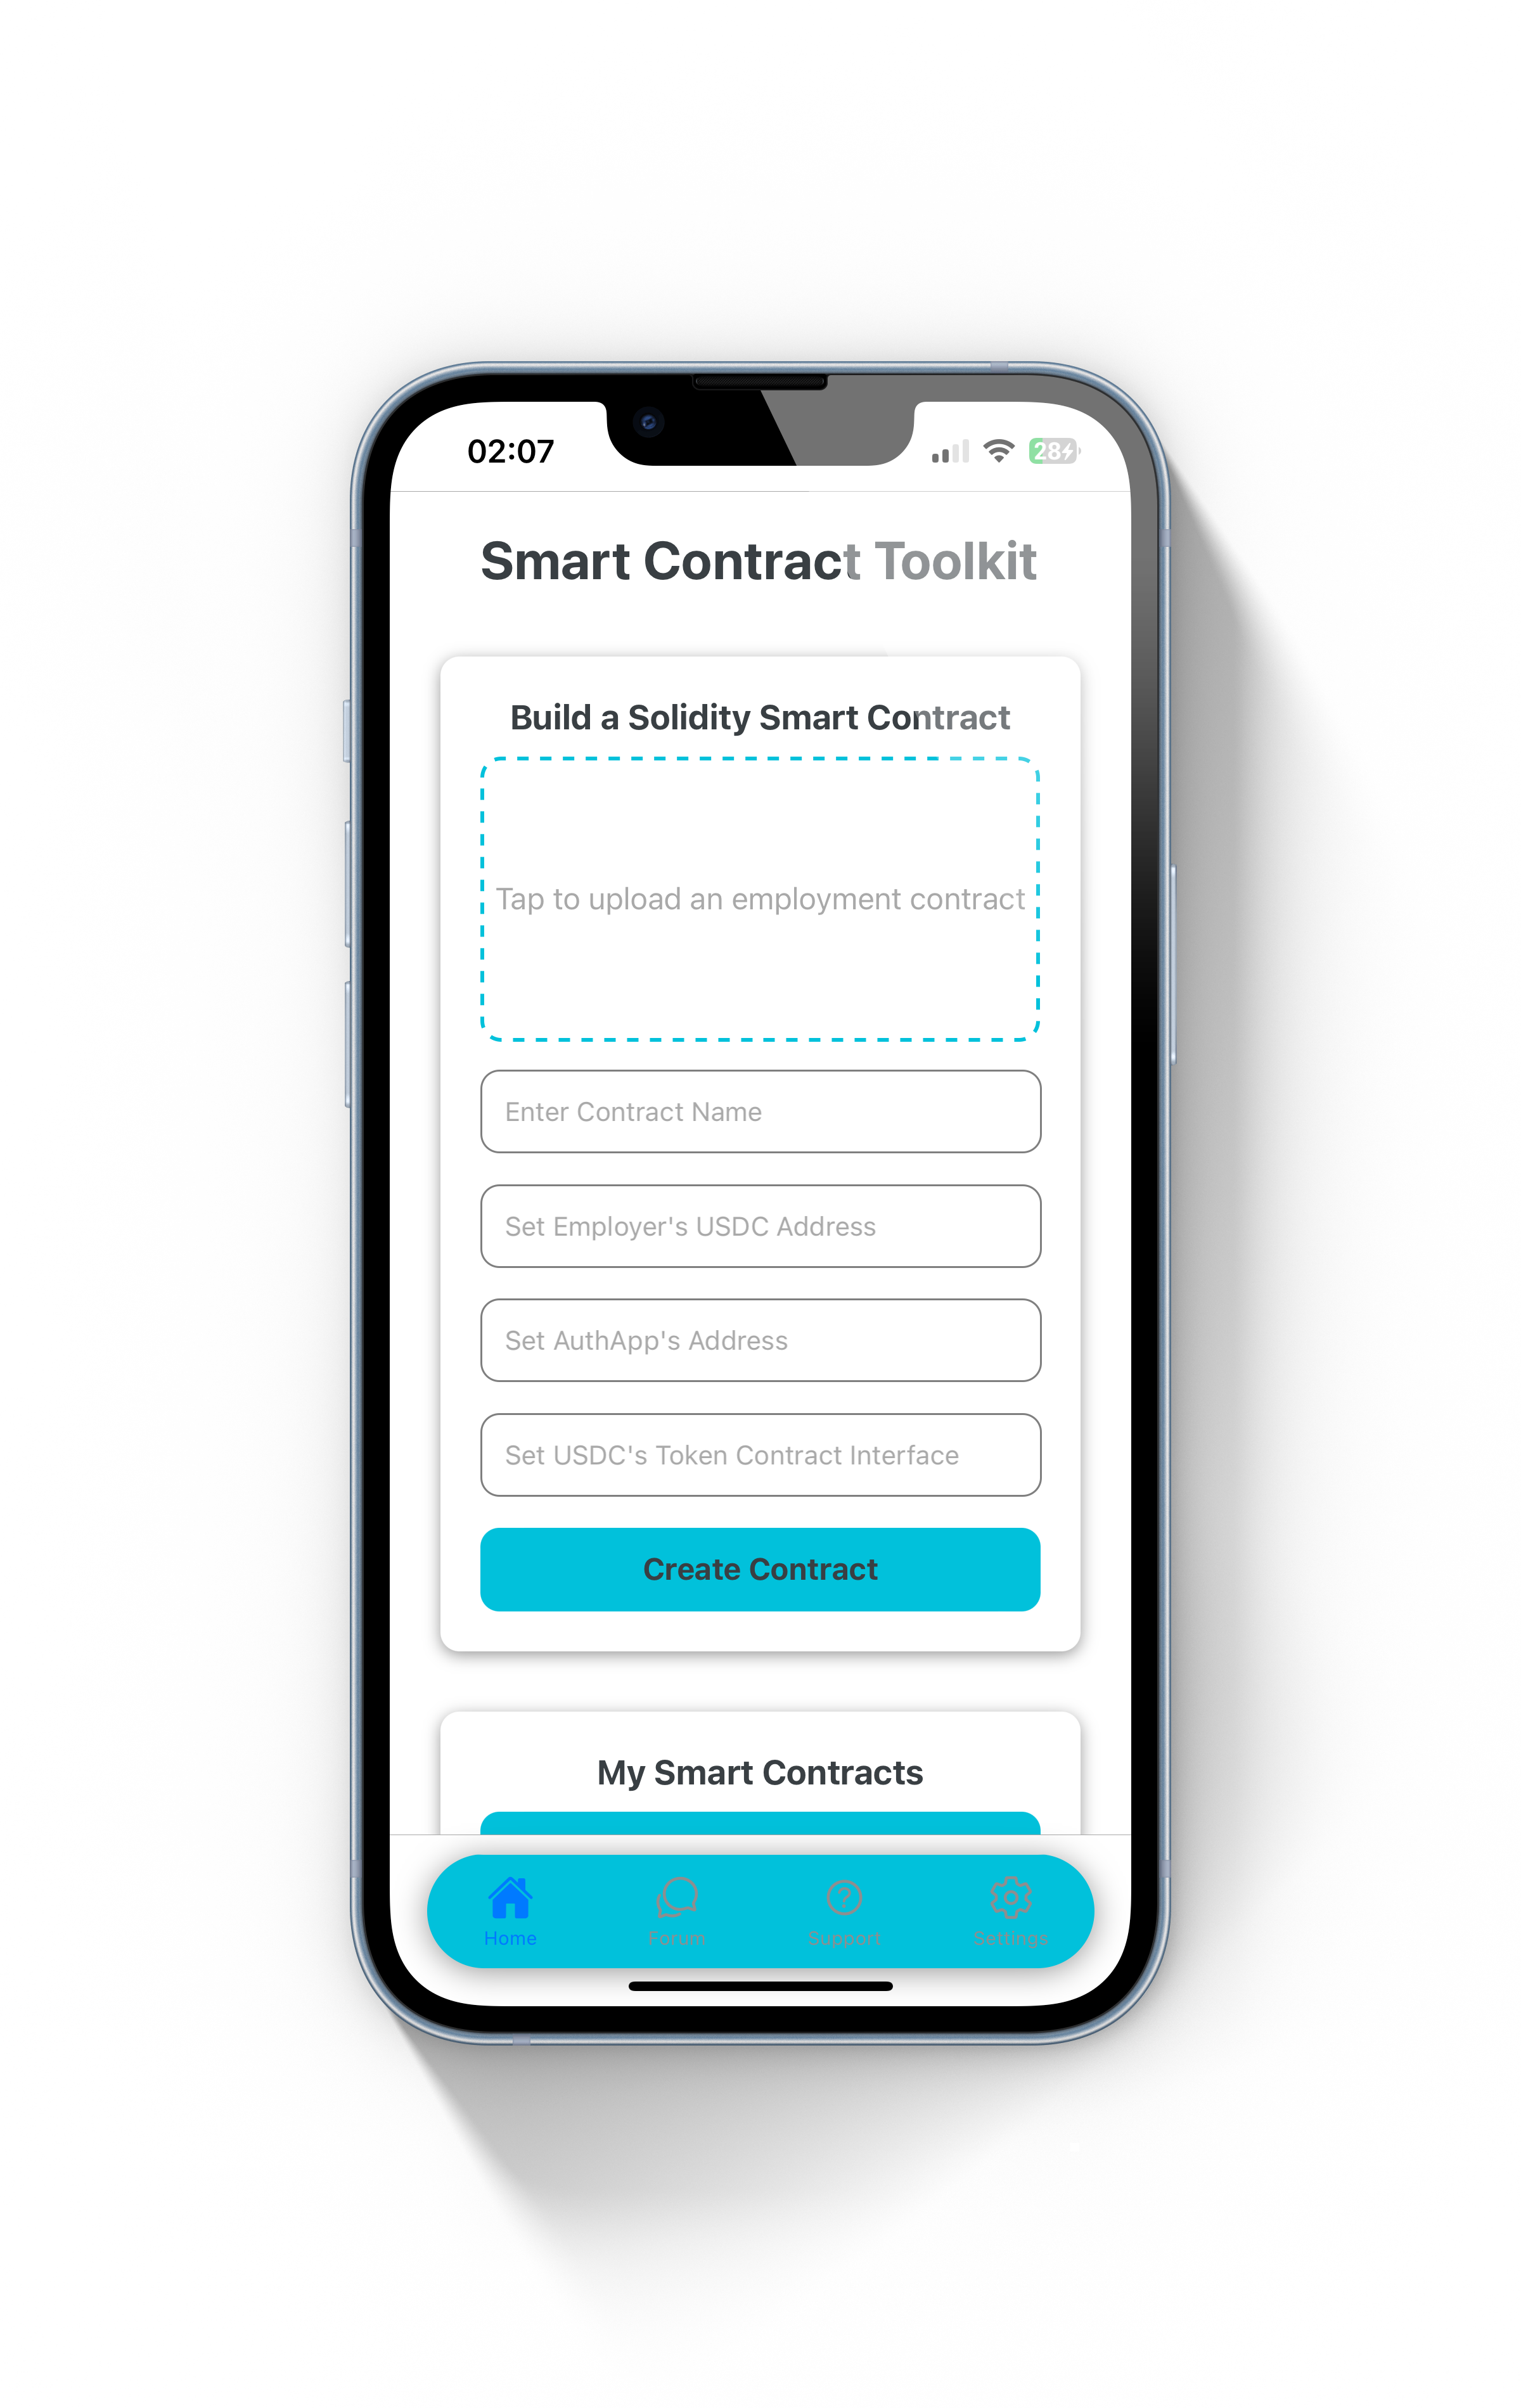
\includegraphics[scale=0.08]{LATEX/Appendices/Images/Software/Frontend/home_screen_1.png}
        \label{fig:home screen 1}
    \end{minipage}\hfill % This inserts a small horizontal space between the minipages
    % Begin the second minipage for the second image
    \begin{minipage}{0.5\textwidth}
        \centering
        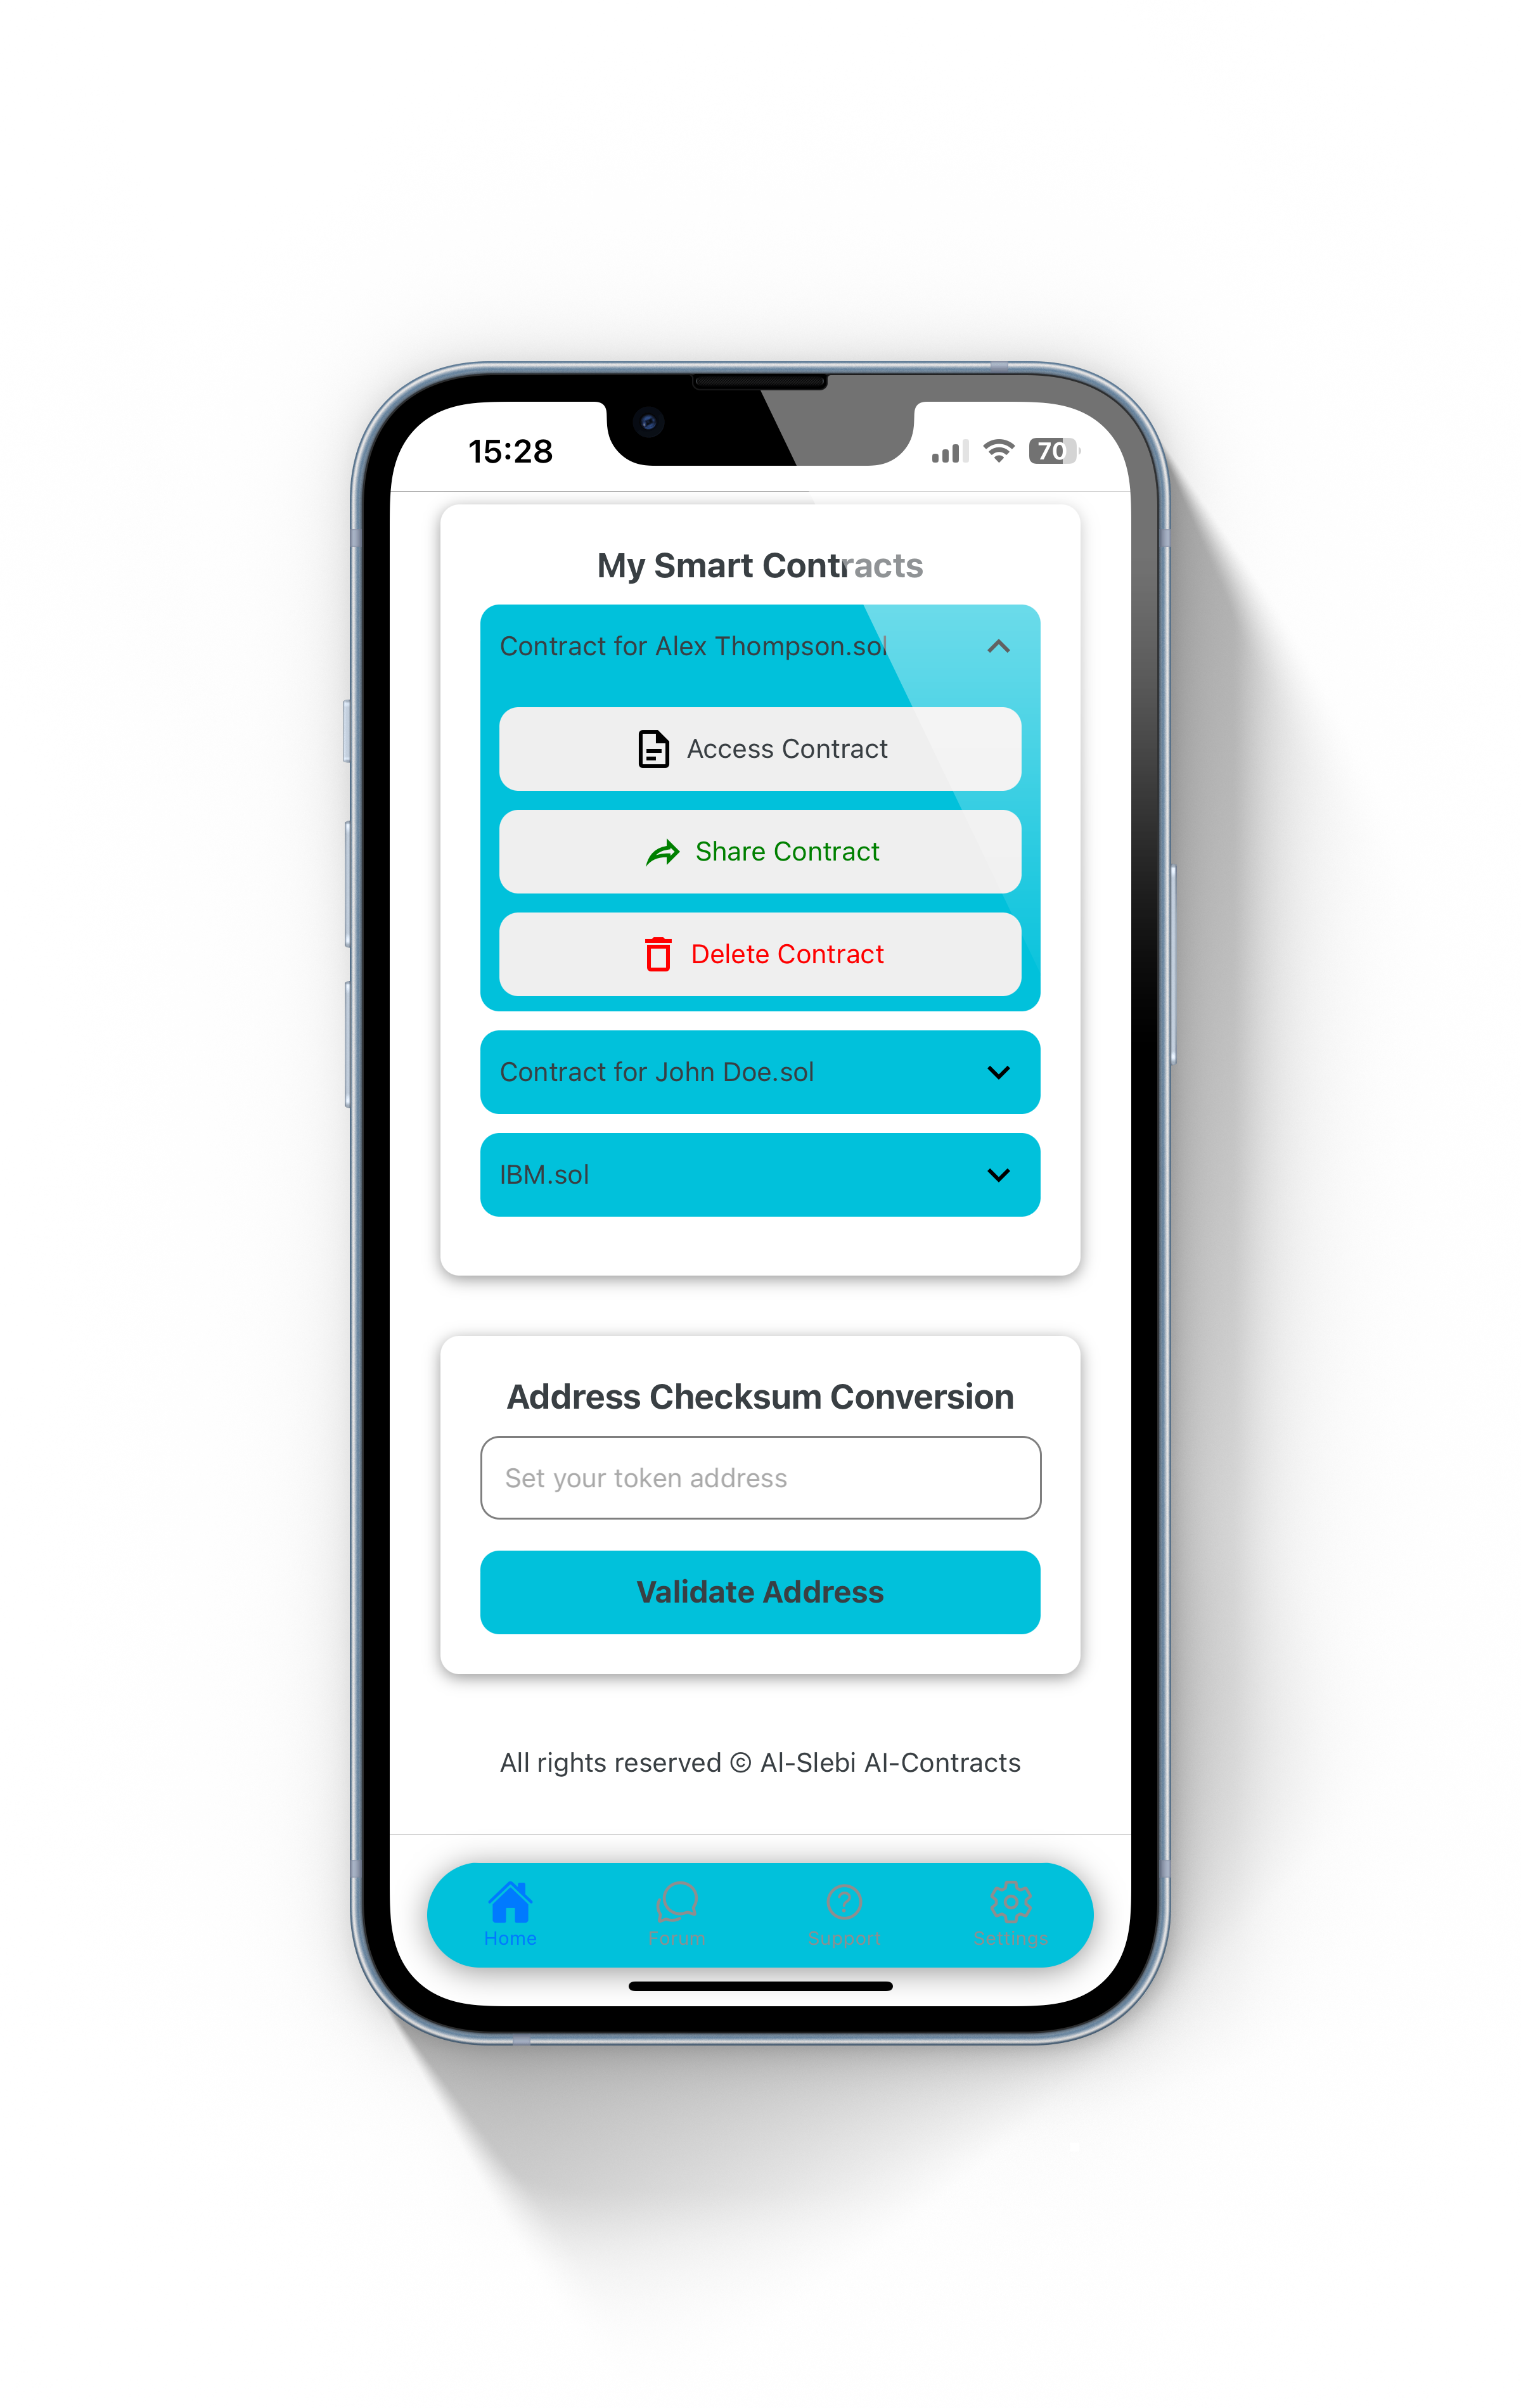
\includegraphics[scale=0.08]{LATEX/Appendices/Images/Software/Frontend/home_screen_2.png}
        \label{fig:home screen 2}
    \end{minipage}
\end{figure}

\begin{figure}[!ht]
    \centering
    % Begin the first minipage for the first image
    \begin{minipage}{0.5\textwidth}
        \centering
        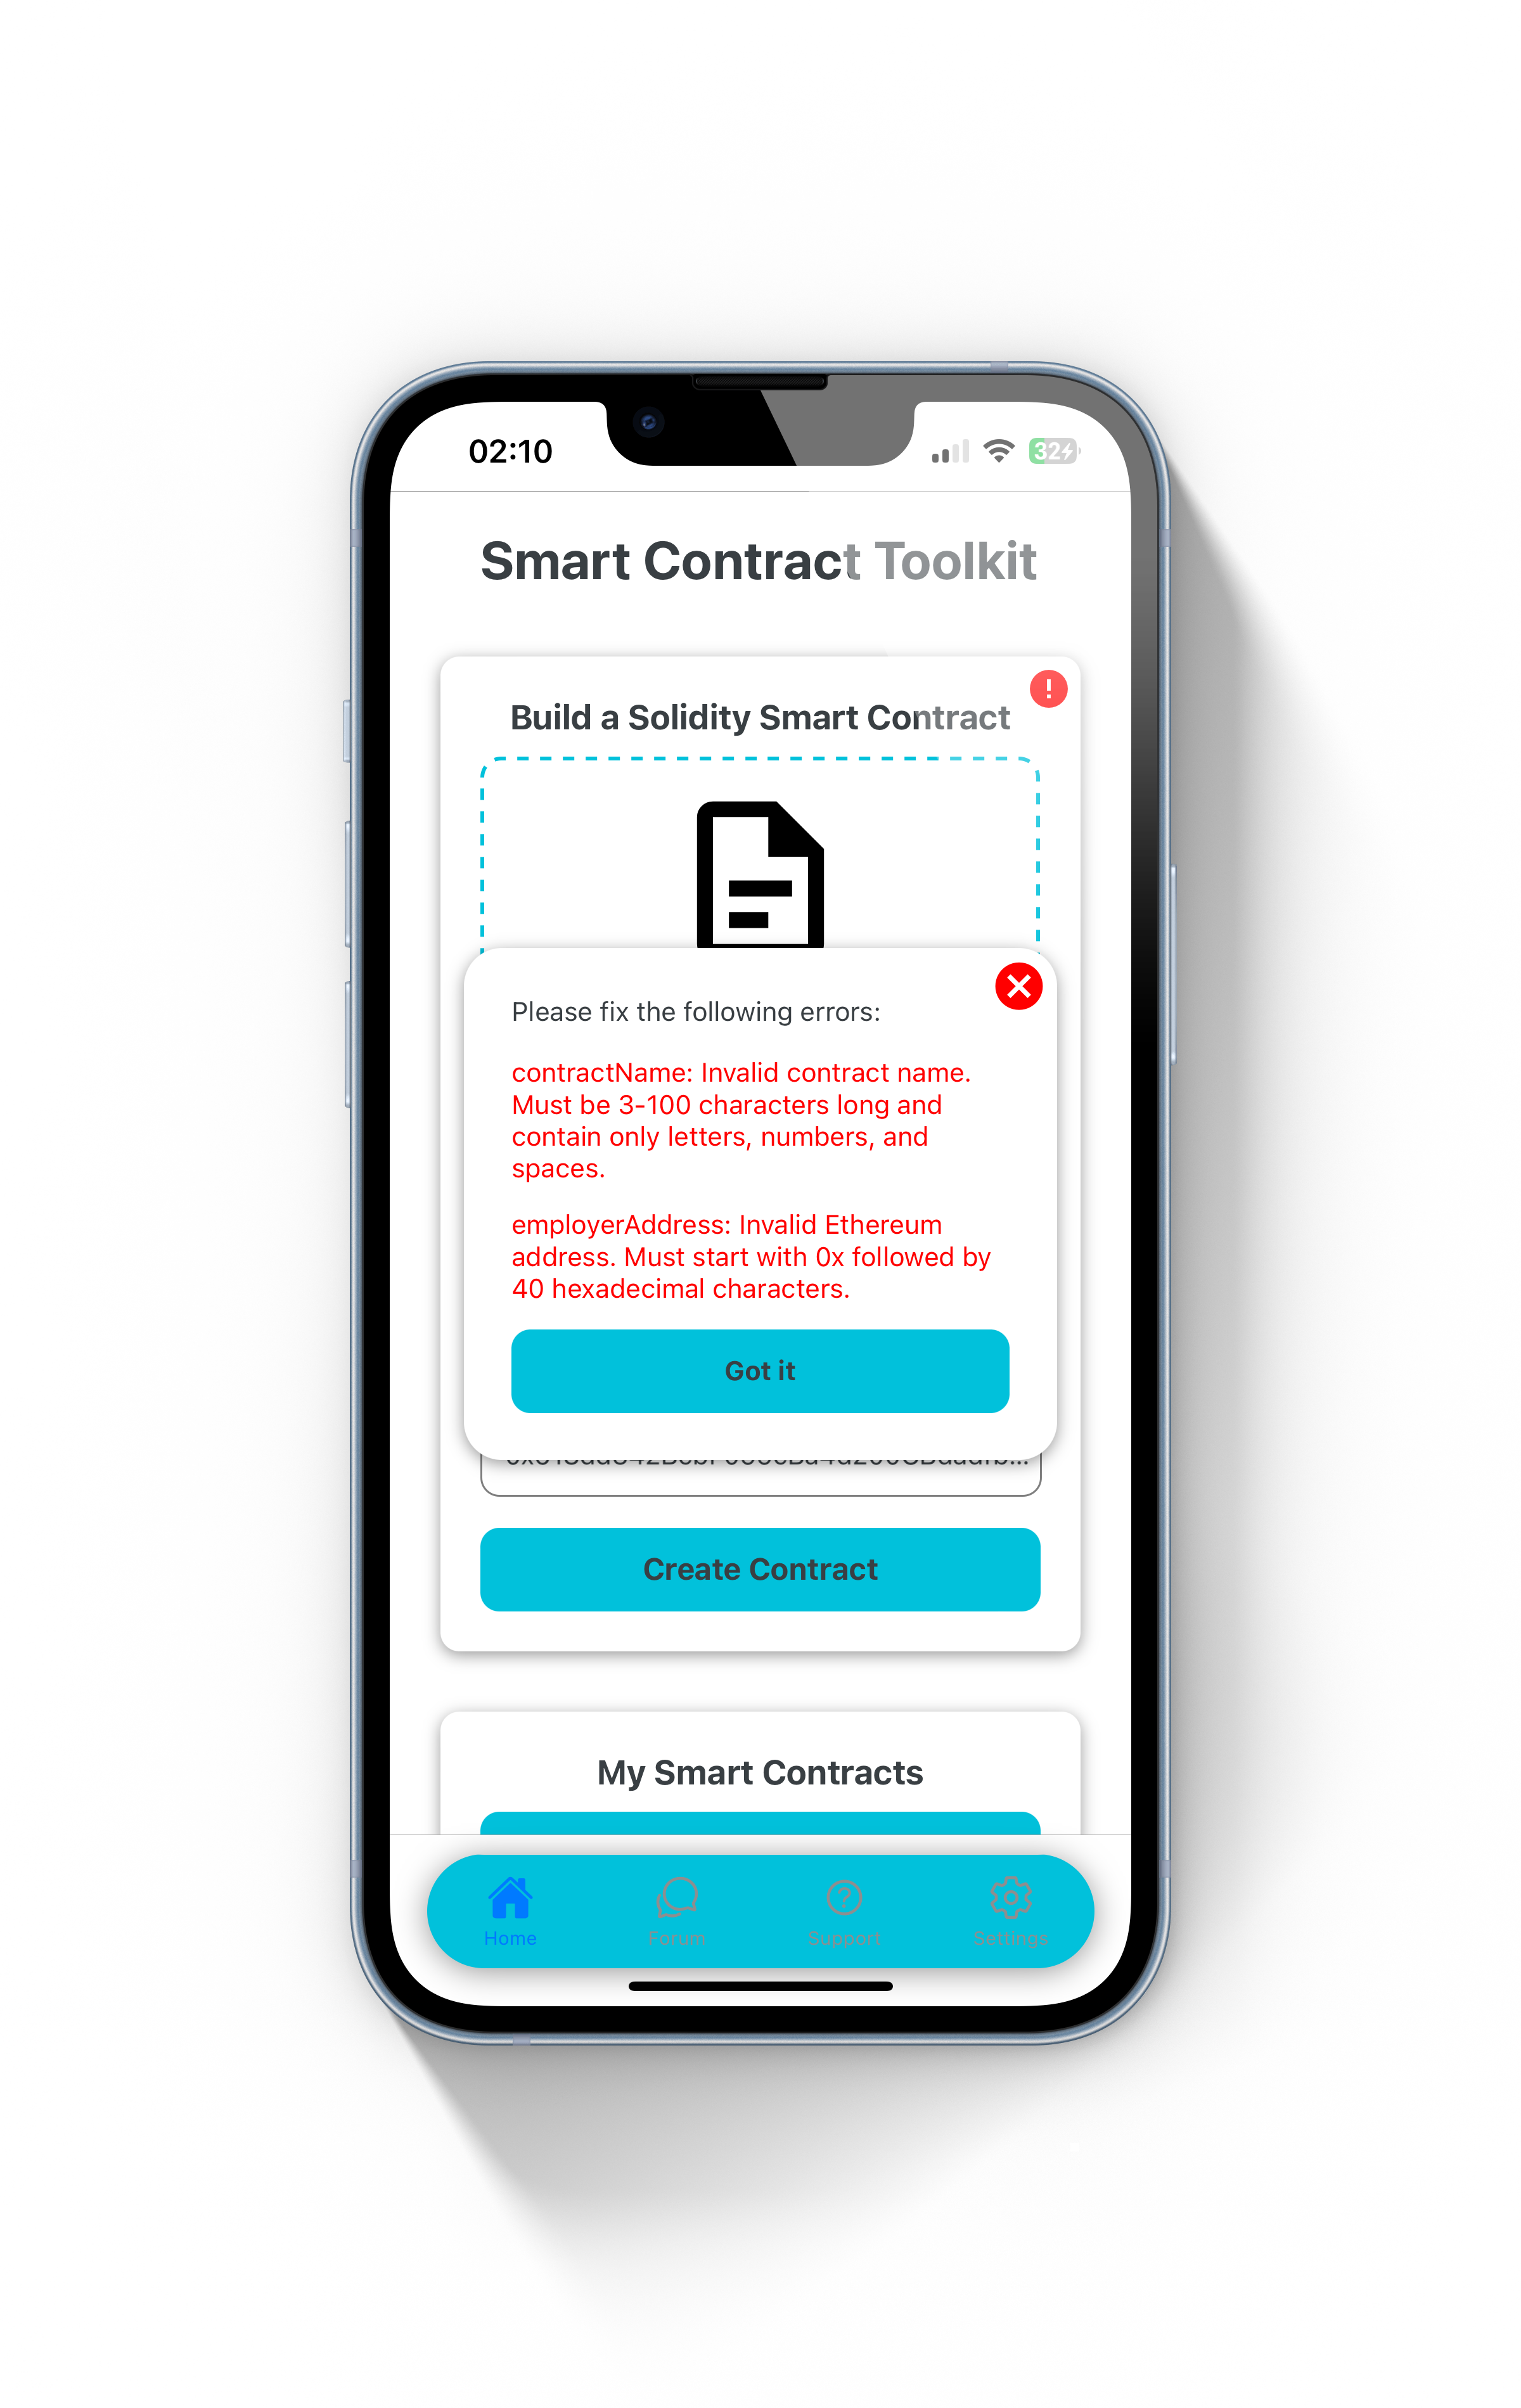
\includegraphics[scale=0.08]{LATEX/Appendices/Images/Software/Frontend/home_screen_3.png}
        \label{fig:home screen 3}
    \end{minipage}\hfill % This inserts a small horizontal space between the minipages
    % Begin the second minipage for the second image
    \begin{minipage}{0.5\textwidth}
        \centering
        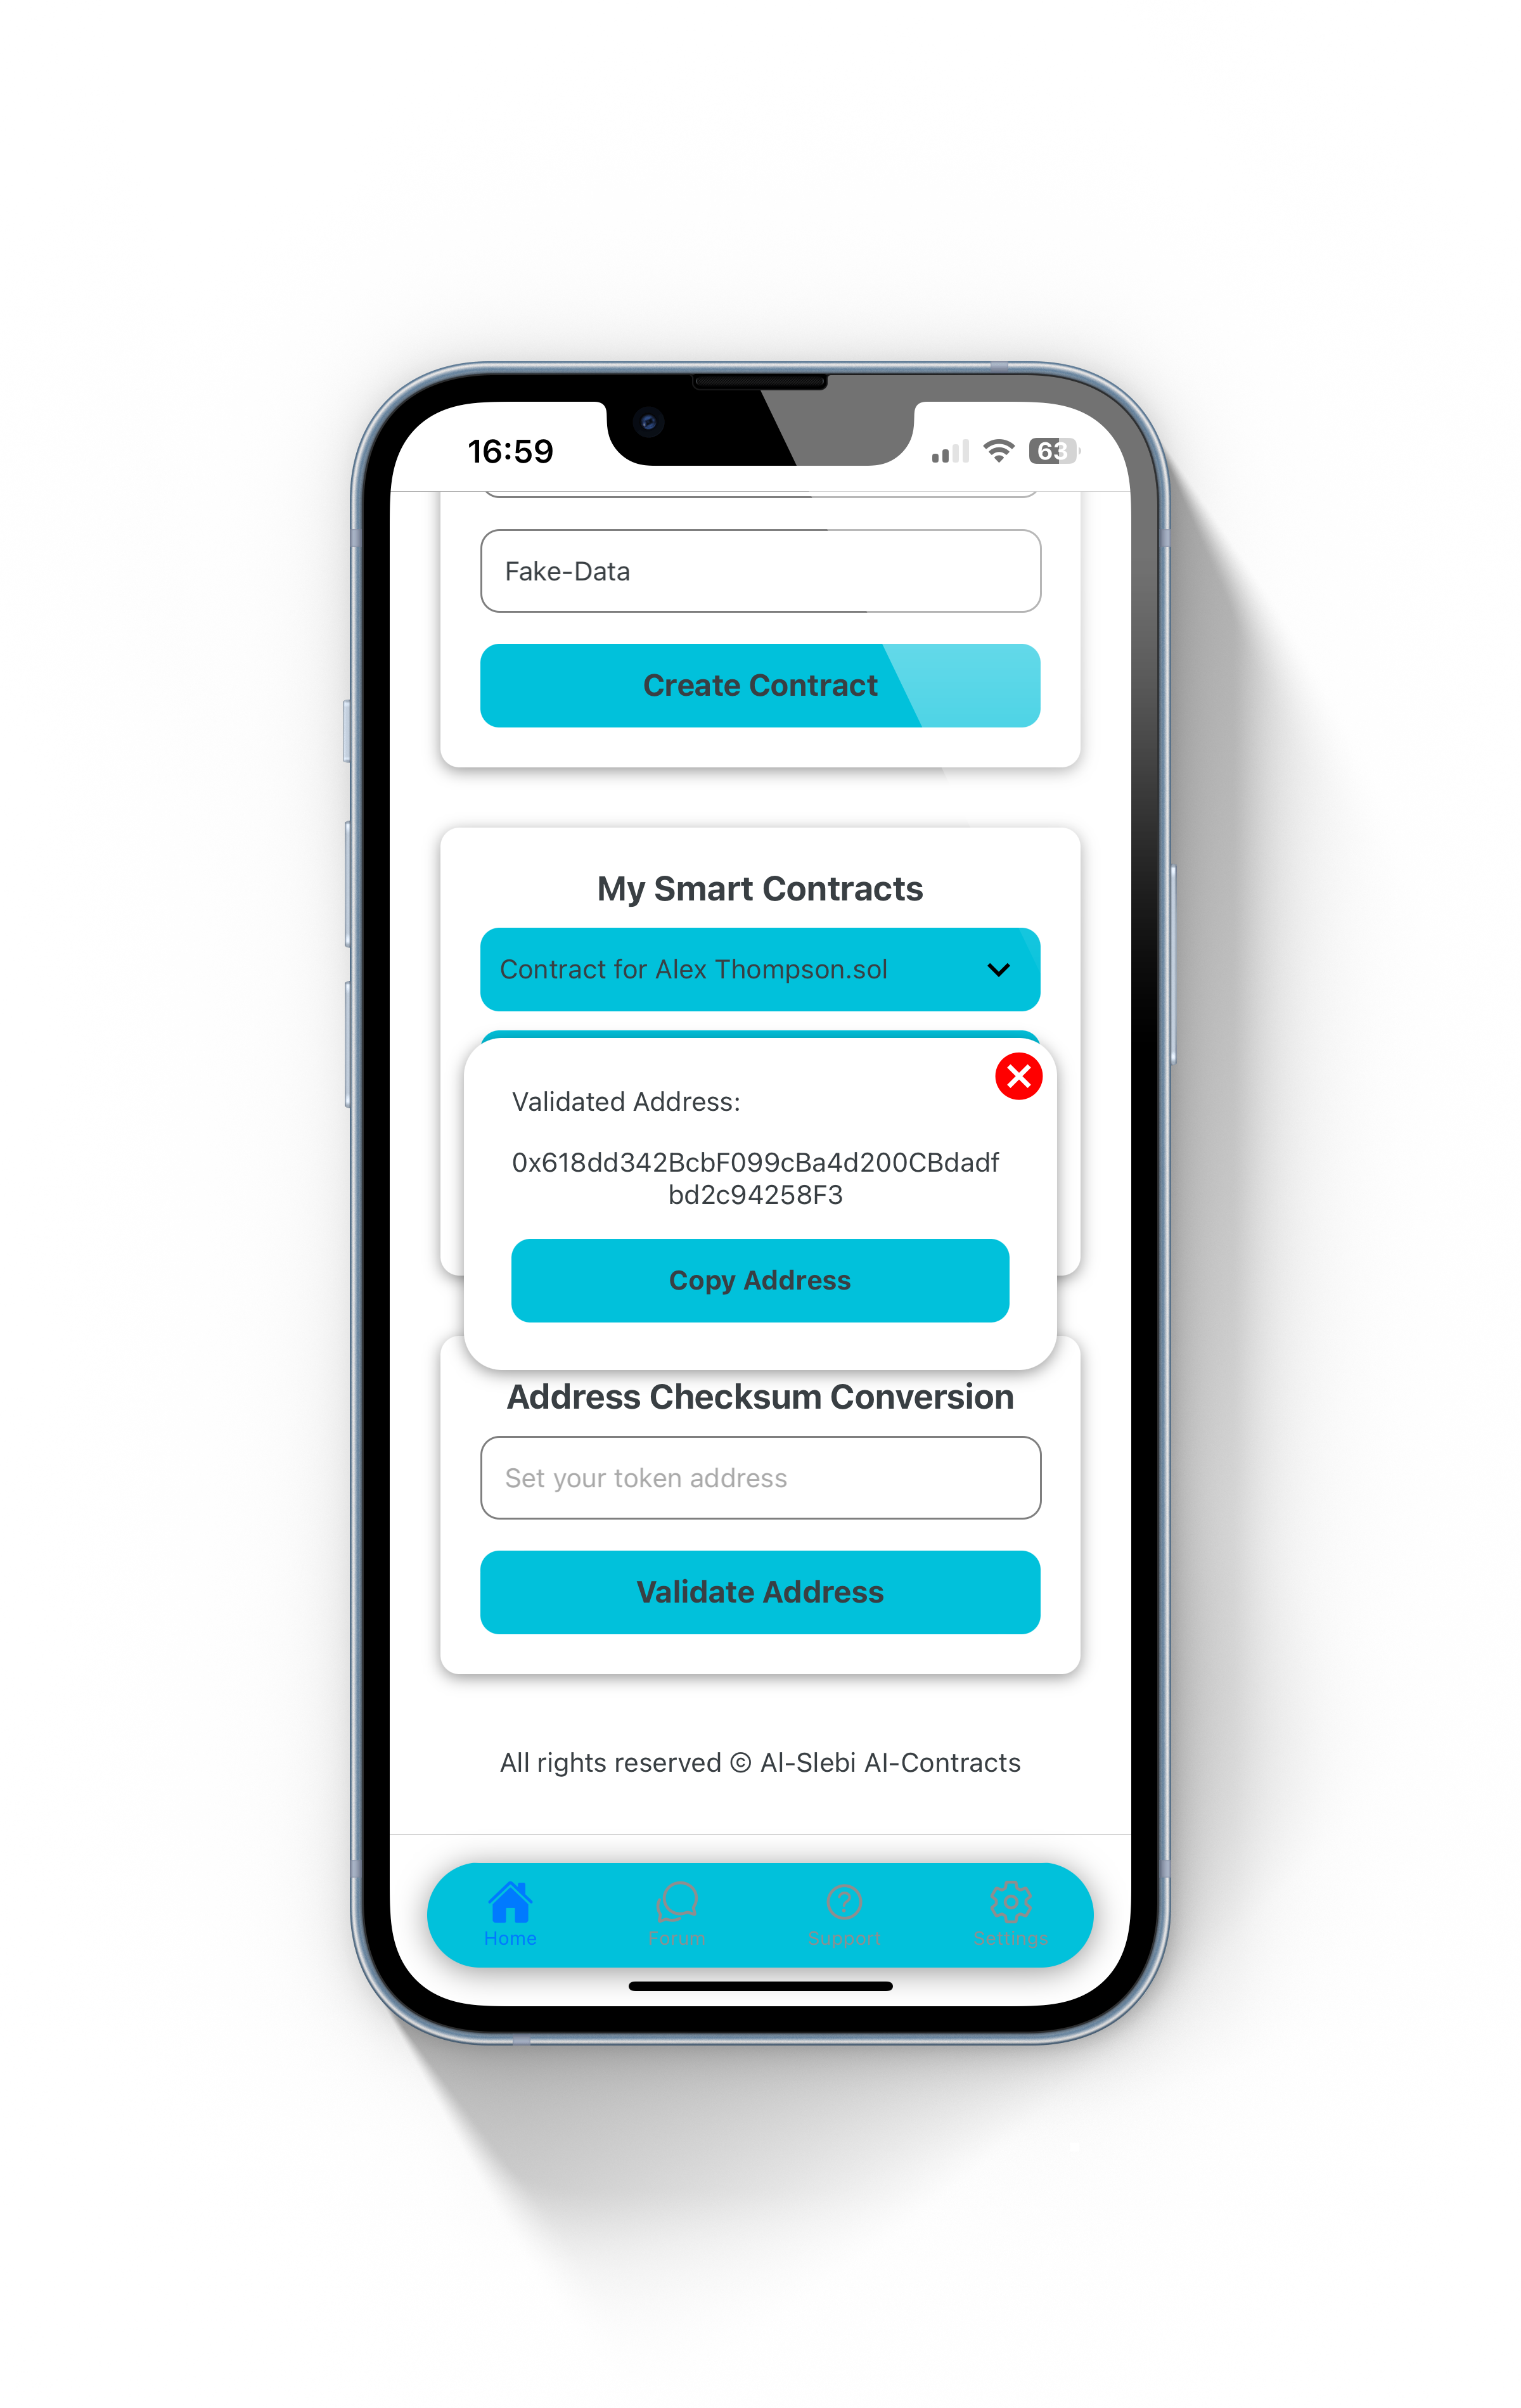
\includegraphics[scale=0.08]{LATEX/Appendices/Images/Software/Frontend/home_screen_4.png}
        \label{fig:home screen 4}
    \end{minipage}
\end{figure}

\newpage
\subsubsection{PostLoginScreens: UseHomeScreen.js}

The file defines the \texttt{useHomeScreen} custom hook, which is used to control the \textit{HomeScreen} component's functionality and state.

\begin{itemize}
    \item \textbf{State Variables:}
    \begin{itemize}
        \item \textit{selectedFile} manages the state of the selected file for contract creation.
        \item \textit{contractName}, \textit{employerAddress}, \textit{authAppAddress}, and \textit{tokenContractInterface} store user inputs for contract details.
        \item Contracts stored on the device are tracked by the \textit{savedContracts} variable.
        \item \textit{isComponentMounted} is a flag to check if the component is mounted.
        \item \textit{showAddressModal} and \textit{validatedAddress} manage the state for displaying and storing the validated Ethereum address.
        \item \textit{errors} and \textit{showErrorDetails} handle validation errors and their visibility.
        \item The Ethereum address that users input to be validated is stored by \textit{addressChecksum} variable.
    \end{itemize}

    \item \textbf{File Selection:}
    \begin{itemize}
        \item Using \textit{ExpoDocumentPicker}, \textit{handleFileSelectDropZone} enables users to choose a file for contract generation. It determines whether the file selection has been cancelled and modifies the \textit{selectedFile} state as necessary. By using \textit{LayoutAnimation}, it also controls the component's animation.
        \begin{itemize}
            \item If the file selection is cancelled and a file is already selected, it clears the \textit{selectedFile} state.
            \item If the file is of type \textit{``text/plain''}, it sets the \textit{selectedFile} state with its details.
        \end{itemize}
    \end{itemize}

    \item \textbf{Upload Contract Data:}
    \begin{itemize}
        \item The function \textit{uploadContractData} is responsible for managing the uploading of contract data. It validates input and verifies that the file and all required fields are supplied. By using \textit{LayoutAnimation}, it also controls the component's animation.
        \item It reads the file content using \textit{FileSystem.readAsStringAsync}, prepares \textit{FormData}, and sends it to the backend server using a \textit{POST} request.
        \item It notifies the user and resets the input fields upon a successful upload.
    \end{itemize}

    \item \textbf{Save Solidity File:}
    \begin{itemize}
        \item \textit{saveSolidityFile} saves the generated Solidity code to the device's file system and controls the animation through \textit{LayoutAnimation}.
        \begin{itemize}
            \item Checks if the file already exists using \textit{FileSystem.getInfoAsync} and overwrites it if necessary.
            \item Saves the file using \textit{FileSystem.writeAsStringAsync}, updates the \textit{savedContracts} state, and alerts the user.
        \end{itemize}
    \end{itemize}

    \item \textbf{Share Contract:}
    \begin{itemize}
        \item \textit{ShareContract} enables users to use \textit{expo-sharing} library to distribute the created contract files. It transmits the file path after determining whether the device possesses the right permission. According to the convention, other applications retrieve the document accordingly from the phone's file system (based on the convention).
    \end{itemize}

    \item \textbf{Open Contract:}
    \begin{itemize}
        \item \textit{openContract} navigates the user to the \textit{EditorScreen} with the path of the selected contract file.
    \end{itemize}

    \item \textbf{Fetch and Sync Contracts:}
    \begin{itemize}
        \item Contracts that have been saved by the user are retrieved from the backend server and synchronised with the local file system using the \textit{fetchAndSyncContracts} function.
        \item It uses the \textit{syncContracts} function to ensure that all contracts are downloaded and saved locally if they do not already exist.
    \end{itemize}

    \item \textbf{Sync Contracts:}
    \begin{itemize}
        \item \textit{syncContracts} iterates over the fetched contracts and saves them locally if they are not already present in the device's file system.
        \begin{itemize}
            \item It uses \textit{FileSystem.readDirectoryAsync} to read the local directory and verify that every contract pulled from the backend is present there.
            \item If a contract is not found locally, it downloads and saves the contract using \textit{saveSolidityFile}.
        \end{itemize}
    \end{itemize}

    \item \textbf{Delete Contract:}
    \begin{itemize}
        \item \textit{handleDeleteContract} deletes a contract both locally and on the backend server, simulating an animation through \textit{LayoutAnimation}.
        \begin{itemize}
            \item It sends a \textit{DELETE} request to the backend server and deletes the local file using \textit{FileSystem.deleteAsync}.
            \item Updates the \textit{savedContracts} state to reflect the deletion.
        \end{itemize}
    \end{itemize}

    \item \textbf{Clean Expo Folder:}
    \begin{itemize}
        \item \textit{cleanExpoFolder} deletes all files in the Expo document directory.
        \begin{itemize}
            \item It reads the directory using \textit{FileSystem.readDirectoryAsync} and deletes each file using \textit{FileSystem.deleteAsync}.
        \end{itemize}
    \end{itemize}

    \item \textbf{Input Validation:}
    \begin{itemize}
        \item \textit{validateInput} is a helper method that updates the state of \textit{errors} variable through the output of the \textit{getValidationErrorMessage} function.
        \item \textit{getValidationErrorMessage} returns appropriate error messages by validating Ethereum addresses, contract names, and JSON formats.
    \end{itemize}

    \item \textbf{Handle Checksum Address:}
    \begin{itemize}
        \item \textit{handleChecksumAddress} validates an Ethereum address by sending a \textit{GET} request to the backend server.
        \begin{itemize}
            \item If the address is valid, it sets the \textit{validatedAddress} state and displays the address in a modal.
            \item If the address is invalid, it displays an error alert.
        \end{itemize}
    \end{itemize}

    \item \textbf{Copy to Clipboard:}
    \begin{itemize}
        \item \textit{copyToClipboard} copies the validated Ethereum address to the clipboard and alerts the user.
    \end{itemize}

    \item \textbf{Additional Helper Functions:}
    \begin{itemize}
        \item \textit{isValidEthereumAddress}, \textit{isValidHexadecimal}, \textit{isValidContractName}, \textit{isValidJson}, and \textit{getValidationErrorMessage} are helper functions used for validating user inputs.
    \end{itemize}
\end{itemize}

In summary, the \textit{useHomeScreen} custom hook simplifies and modularises the code by encapsulating the state management and necessary functionalities needed for the \textit{HomeScreen} UI component.

\subsubsection{PostLoginScreens: ContractItem.js}

Users can open, share, delete, and expand contract details through this component. 

\begin{itemize}
    \item \textbf{State Variables and Refs:}
    \begin{itemize}
        \item \textit{expanded}: A state variable to track whether the contract details are expanded or collapsed.
        \item \textit{animationController}: An animated value to control the height of the contract details section.
        \item \textit{opacityAnimation} and \textit{heightAnimation}: During deletion, the opacity and height are controlled by these states.
        \item \textit{isMounted}: A reference for detecting animations and halting them.
    \end{itemize}

    \item \textbf{useEffect Hook:}
    \begin{itemize}
        \item The \textit{useEffect} hook sets \textit{isMounted} to \textit{false} and stops the animation controller when the component unmounts.
    \end{itemize}

    \item \textbf{toggleExpand:}
    \begin{itemize}
        \item This function initiates an animation to expand or compress the details section. It also refreshes the expanded state.
        \item Uses \textit{Animated.timing} to animate the \textit{animationController} value over 500 milliseconds.
    \end{itemize}

    \item \textbf{initiateDeletion:}
    \begin{itemize}
        \item This method shows an alert to confirm the deletion of a contract.
        \item If the user confirms, it triggers the \texttt{handleDeletionAnimation}.
    \end{itemize}

    \item \textbf{handleDeletionAnimation:}
    \begin{itemize}
        \item It performs an animation to fade out and collapse the contract item before deleting it.
        \item Uses \textit{Animated.parallel} to run the opacity and height animations simultaneously over 300 milliseconds.
        \item Calls the \textit{deleteContract} function to remove the contract after the animation completes.
    \end{itemize}

    \item \textbf{animatedHeight:}
    \begin{itemize}
        \item This interpolates the \textit{animationController} value to animate the height of the contract details section between 0 and 180 pixels.
    \end{itemize}

    \item \textbf{Return Statement:}
    \begin{itemize}
        \item The \textit{ContractItem} component renders a \textit{TouchableOpacity} container that toggles the expansion of the contract details.
        \item It displays the contract name and an icon indicating the expanded state.
        \item The animated view expands to show additional actions: \textit{Access Contract}, \textit{Share Contract}, and \textit{Delete Contract}.
    \end{itemize}
\end{itemize}

\subsubsection{PostLoginScreens: EditorScreen.js}

The \texttt{EditorScreen} is a functional component that uses \textit{navigation} and \textit{route} as props.

\begin{itemize}
    \item \textbf{Parameters and Hook:}
    \begin{itemize}
        \item The file path of the contract to be edited is retrieved from \textit{route.params}.
        \item The custom hook \textit{useEditorScreen} is called with the file path and theme as arguments to fetch the HTML content of the code and the loading state.
    \end{itemize}

    \item \textbf{Return Statement:}
    \begin{itemize}
        \item A view container with conditional rendering based on the \textit{isLoading} state is returned by the component.
        \begin{itemize}
            \item If \textit{isLoading} is true, an \textit{ActivityIndicator} is displayed.
            \item If \textit{isLoading} is false, a \textit{WebView} component is rendered to display the HTML content of the code.
        \end{itemize}
        \item The \textit{WebView} component uses \textit{originWhitelist} to allow all origins and sets the source to the HTML content obtained from the custom hook.
        \item The \textit{WebView} and \textit{ActivityIndicator} are styled using the shared and local styles.
        
        \item A separator line is included at the bottom using the \textit{sharedStyles.separatorLine}.
    \end{itemize}
\end{itemize}

\begin{figure}[!ht]
    \centering
    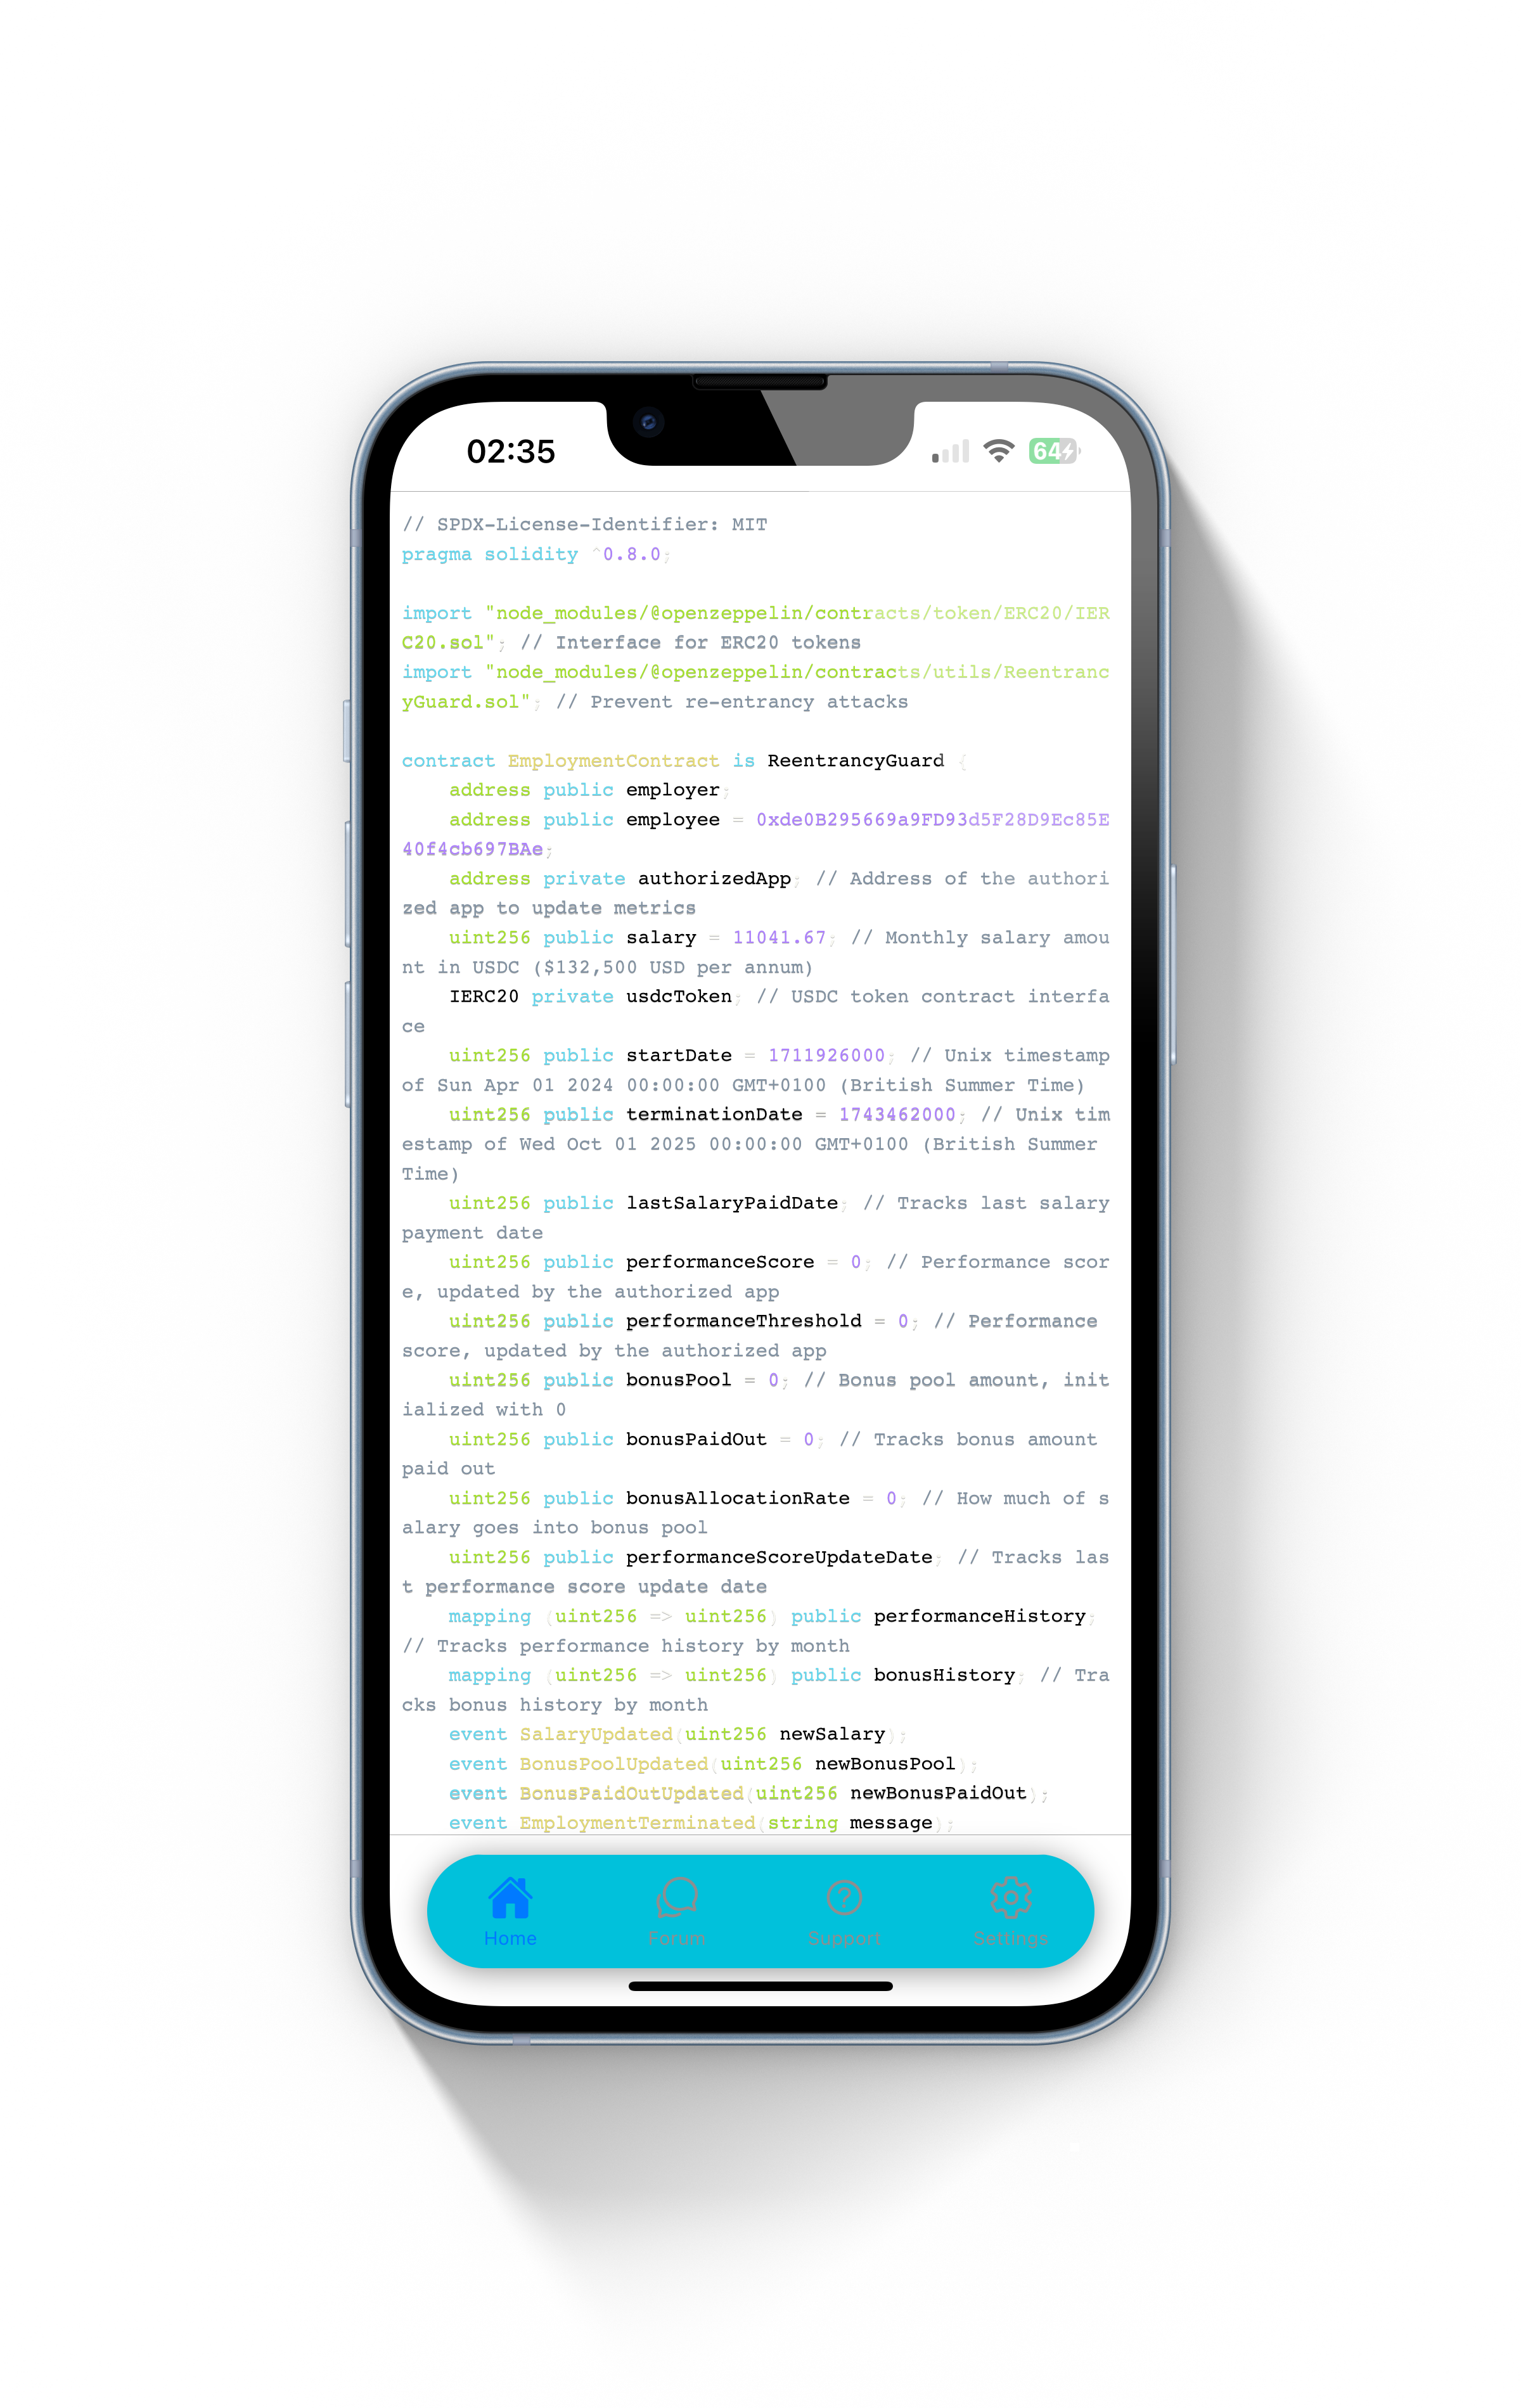
\includegraphics[width=0.43\textwidth]
    {LATEX/Appendices/Images/Software/Frontend/editor_screen.png}
    \label{fig:editor screen}
\end{figure}

\subsubsection{PostLoginScreens: UseEditorScreen.js}

A customised hook that loads and formats contract file content for \textit{web view} presentation is defined in the \texttt{UseEditorScreen.js} file

\begin{itemize}
    \item \textbf{State Variables:}
    \begin{itemize}
        \item \textit{fileContent}: Stores the raw content of the contract file.
        \item \textit{codeHtml}: Stores the HTML content generated from the raw contract file.
        \item \textit{isLoading}: A boolean flag indicating whether the file content is still loading.
    \end{itemize}

    \item \textbf{useEffect Hook for Loading File Content:}
    \begin{itemize}
        \item The first \textit{useEffect} hook is responsible for loading the content of the contract file specified by \textit{filePath}.
        \item It defines an asynchronous function, \textit{loadFileContent}, which reads the file content using \textit{FileSystem.readAsStringAsync}.
        \item The file content is then stored in the \textit{fileContent} state variable.
        \item If an error occurs during file reading, an alert is displayed, and the error is logged to the console.
    \end{itemize}

    \item \textbf{useEffect Hook for Generating HTML Content:}
    \begin{itemize}
        \item The second \textit{useEffect} hook is responsible for generating the HTML content from the raw file.
        \item It runs whenever the \textit{theme} or \textit{fileContent} changes.
        \item The file content is escaped to prevent HTML injection by replacing special characters with their corresponding HTML entities.
        \item An HTML template is created, which includes:
        \begin{itemize}
            \item A link to the Prism CSS file for syntax highlighting.
            \item Scripts for \textit{Prism} and \textit{Solidity} syntax highlighting.
            \item Inline styles for setting the background and text colours, font properties, and ensuring proper word wrapping and formatting.
        \end{itemize}
        \item The escaped content is embedded within a \textit{<pre><code>} block for syntax highlighting.
        \item The generated HTML template is stored in the \textit{codeHtml} state variable.
        \item The \textit{isLoading} state is set to \textit{false}.
    \end{itemize}

    \item \textbf{Return Values:}
    \begin{itemize}
        \item The hook returns the \textit{codeHtml} and \textit{isLoading} values, which are used by the \textit{EditorScreen} component to display the contract code.
    \end{itemize}
\end{itemize}

\subsubsection{PostLoginScreens: ForumScreen.js}

The \textit{ForumScreen} is a functional component that takes \textit{navigation} as a prop. Post management features and state variables are provided by the \textit{useForumScreen} hook.

\begin{itemize}
    \item \textbf{Loading State:}
    \begin{itemize}
        \item If the \textit{loading} state is true, a loading message is displayed.
    \end{itemize}

    \item \textbf{Rendering Posts:}
    \begin{itemize}
        \item The \textit{renderPost} function handles posts rendering.
        \item The title and description of each post are shown within a card container.
        \item Posts include:
        \begin{itemize}
            \item The like button, which toggles the post's like state and updates the like count.
            \item The delete button, which is only shown if the user is the author of the post, allowing them to delete it.
            \item The comment button, which navigates the user to the comment screen for the post.
        \end{itemize}
    \end{itemize}

    \item \textbf{Return Statement:}
    \begin{itemize}
        \item The component returns a \textit{View} container with the following elements:
        \begin{itemize}
            \item A header text displaying \textit{``Community Forum''}.
            \item Input fields and a button for creating a new post.
            \begin{itemize}
                \item \textit{TextInput} fields for the post title and description.
                \item A \textit{TouchableOpacity} button for submitting the new post.
            \end{itemize}
            \item A separator line.
            \item A \textit{FlatList} component for displaying the list of posts.
            \begin{itemize}
                \item The \textit{FlatList} uses the \textit{renderPost} function to render each item.
                \item A footer component with padding is added to the end of the list.
            \end{itemize}
            \item Another separator line at the bottom.
        \end{itemize}
    \end{itemize}
\end{itemize}

\begin{figure}[!ht]
    \centering
    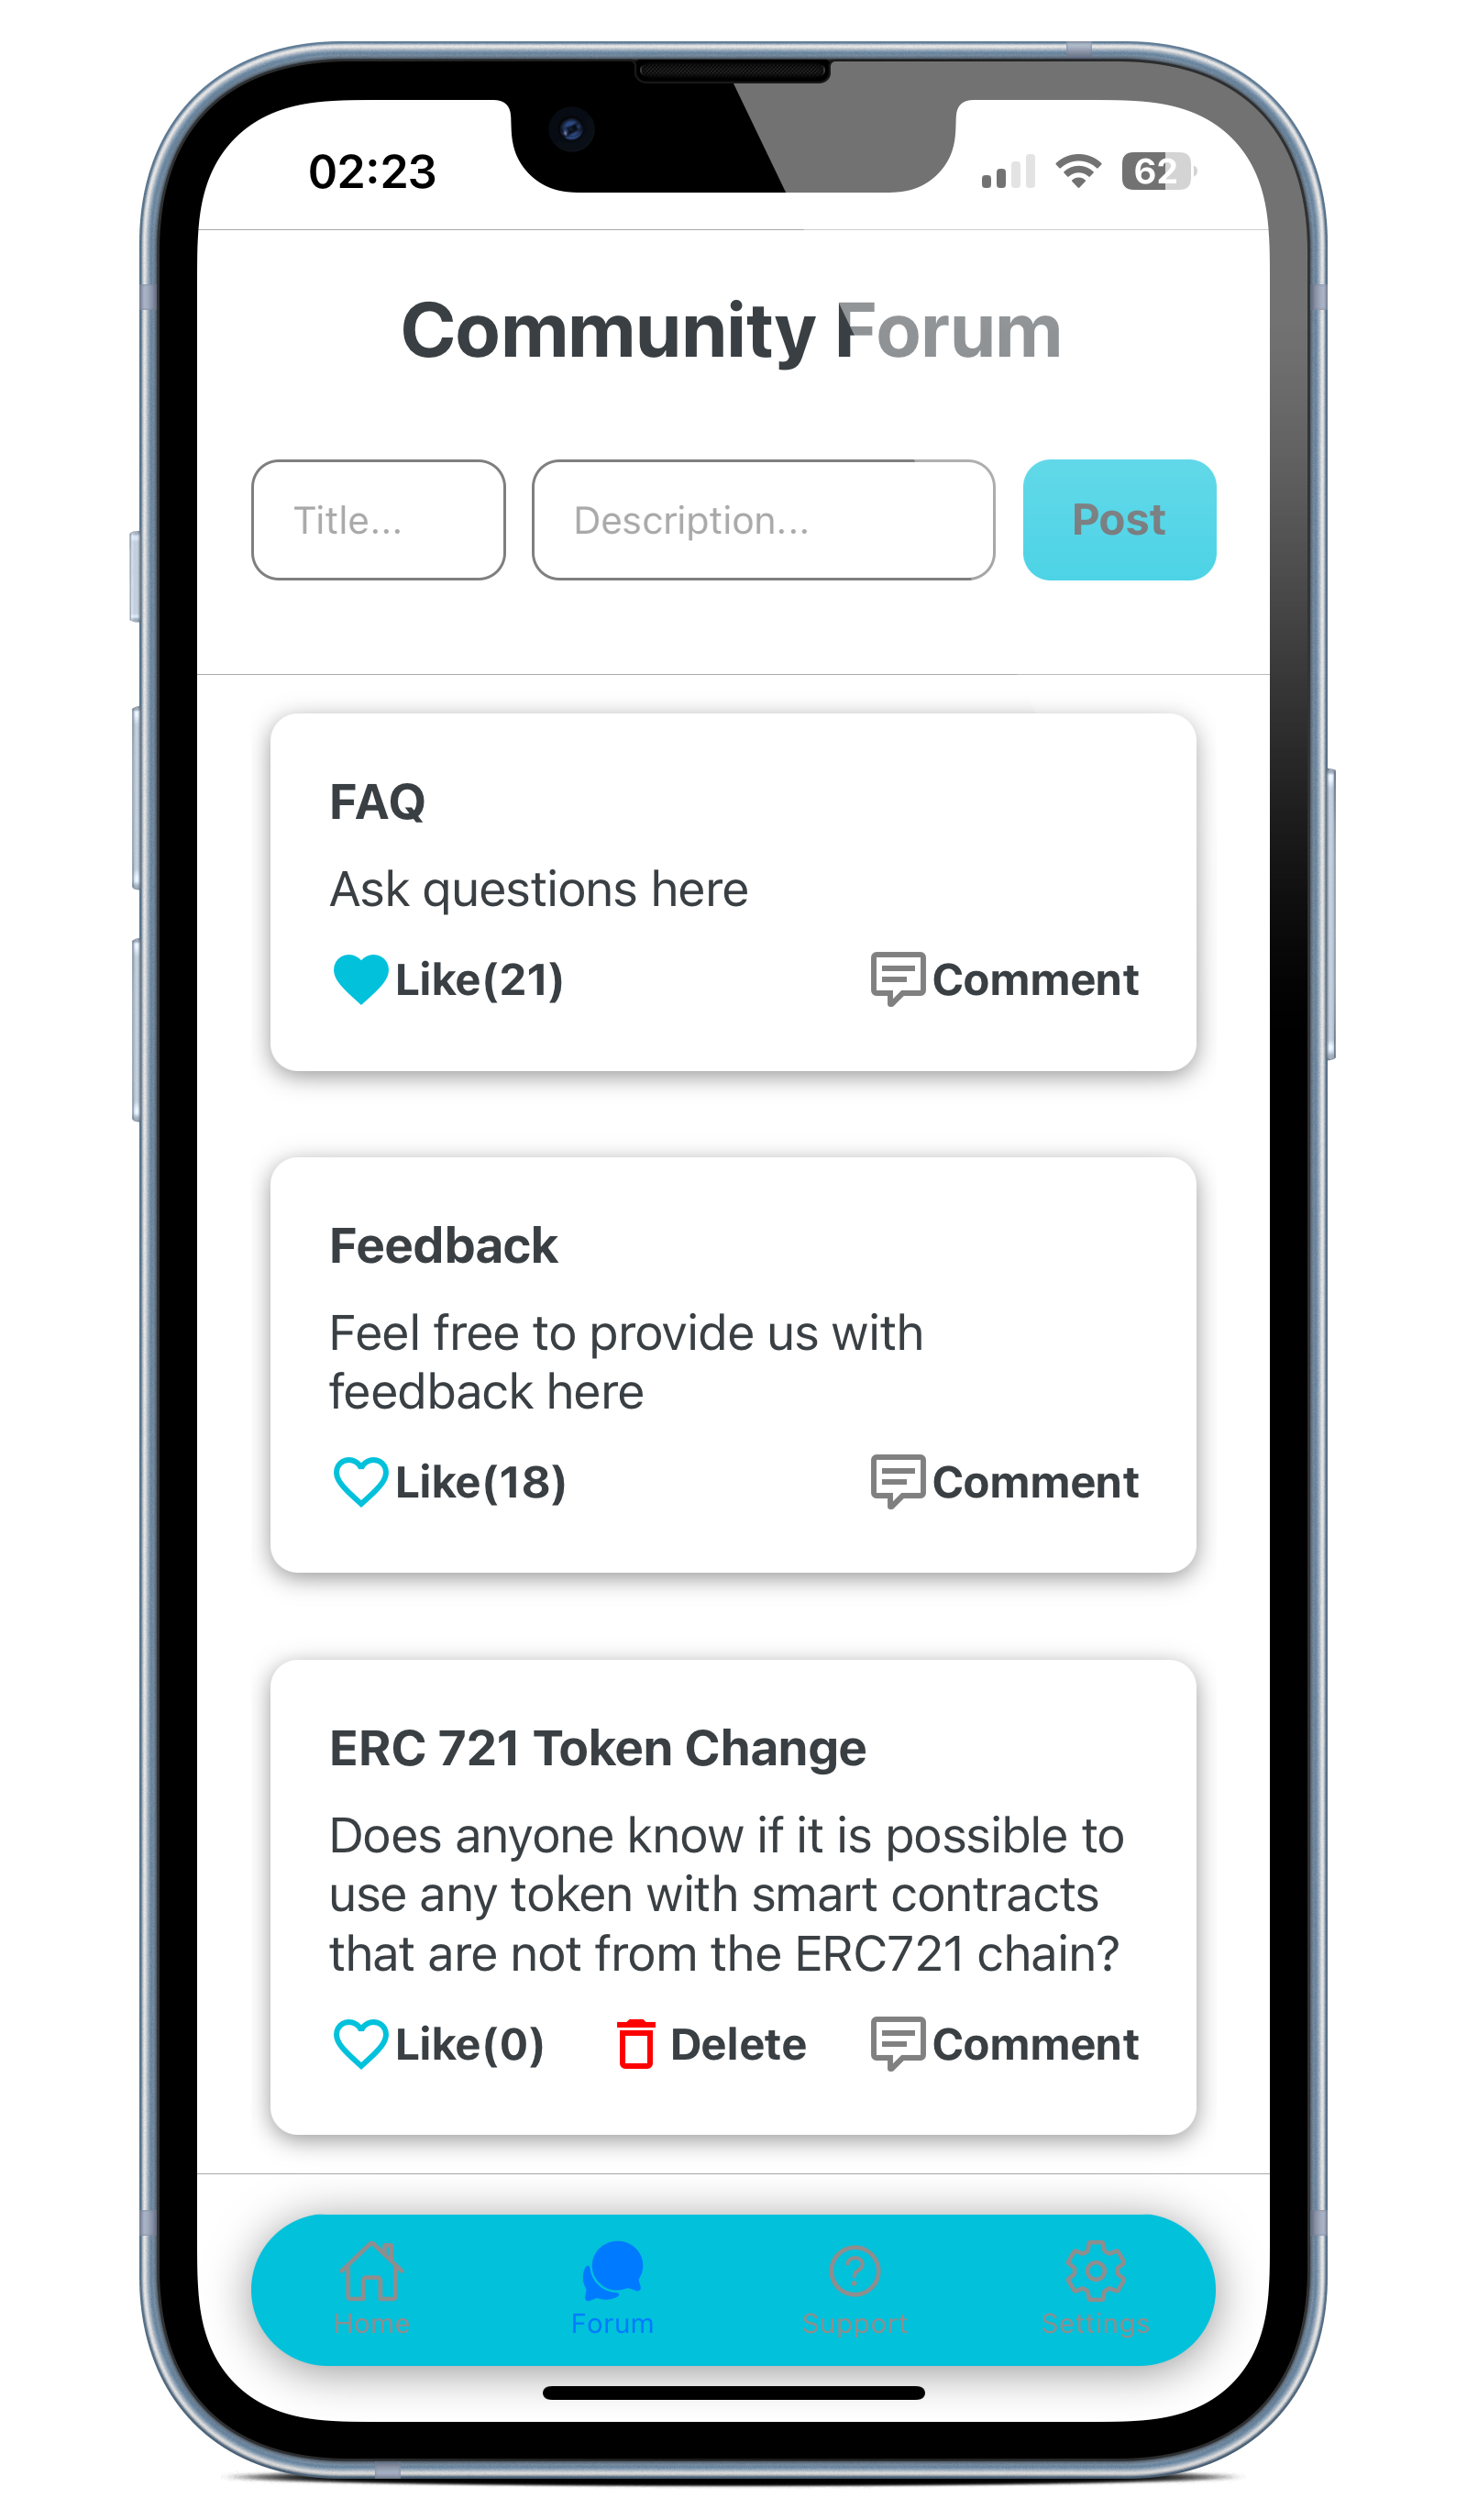
\includegraphics[width=0.3\textwidth]
    {LATEX/Appendices/Images/Software/Frontend/forum_screen_2.png}
    \label{fig:forum screen}
\end{figure} 

\newpage
\subsubsection{PostLoginScreens: UseForumScreen.js}

The \texttt{UseForumScreen.js} file defines a custom hook, \textit{useForumScreen}, and a context provider, \textit{PostProvider}, which manage the state and functionality of the forum screen.

\begin{itemize}
    \item \textbf{Context Creation:}
    \begin{itemize}
        \item \textit{PostContext}: Creates a context for managing and accessing forum-related state and functions.
        \item \textit{useForumScreen}: A custom hook that allows components to consume the \textit{PostContext}.
    \end{itemize}

    \item \textbf{State Variables:}
    \begin{itemize}
        \item \textit{posts}: An array to store the list of posts.
        \item \textit{loading}: A boolean flag to indicate if the posts are being fetched.
        \item \textit{newPostTitle}: A string to store the title of a new post.
        \item \textit{newPostDescription}: A string to store the description of a new post.
    \end{itemize}

    \item \textbf{useEffect Hook for Fetching Posts:}
    \begin{itemize}
        \item The \textit{useEffect} hook calls \textit{fetchPosts} to load the list of posts when the component mounts.
    \end{itemize}

    \item \textbf{Fetching Posts:}
    \begin{itemize}
        \item \textit{fetchPosts} is an asynchronous function.
        \begin{itemize}
            \item It sets \textit{loading} to \textit{true} before making the request.
            \item Retrieves the authentication token from \textit{SecureStore}.
            \item Makes a \textit{GET} request to the backend to fetch the posts.
            \item Sorts the posts by \textit{like\_count} in descending order.
            \item Updates the \textit{posts} state with the sorted posts and sets \textit{loading} to \textit{false}.
            \item Logs any errors encountered during the fetch.
        \end{itemize}
    \end{itemize}

    \item \textbf{Creating a Post:}
    \begin{itemize}
        \item \texttt{createPost} is an asynchronous function.
        \begin{itemize}
            \item it validates that the title and description are not empty.
            \item Resets the \textit{newPostTitle} and \textit{newPostDescription} states after validation.
            \item Makes a \textit{POST} request to the backend with the new post's title and description.
            \item If the request is successful, it adds the new post to the \textit{posts} state using \textit{LayoutAnimation} for a smooth transition.
            \item Logs any errors encountered during the post creation.
        \end{itemize}
    \end{itemize}

    \item \textbf{Liking a Post:}
    \begin{itemize}
        \item \texttt{handleLikePost} is an asynchronous function to like or unlike a post.
        \begin{itemize}
            \item Updates the local \textit{posts} state optimistically to reflect the like or unlike action immediately.
            \item Makes a \textit{POST} or \textit{DELETE} request to the backend based on whether the post is liked or unliked.
            \item If the request fails, reverts the optimistic update.
            \item Logs any errors encountered during the like or unlike action.
        \end{itemize}
    \end{itemize}

    \item \textbf{Deleting a Post:}
    \begin{itemize}
        \item \texttt{handleDeletePost} is an asynchronous function to delete a post.
        \begin{itemize}
            \item Makes a \textit{DELETE} request to the backend to delete the post.
            \item If the request is successful, removes the post from the \texttt{posts} state using \textit{LayoutAnimation} for a smooth transition.
            \item Logs any errors encountered during the post deletion.
        \end{itemize}
    \end{itemize}

    \item \textbf{Context Provider:}
    \begin{itemize}
        \item \texttt{PostProvider} wraps its children with \textit{PostContext.Provider} and provides the state variables and functions for managing posts.
        \item The provider value includes \textit{posts}, \textit{loading}, \textit{createPost}, \textit{handleLikePost}, \textit{handleDeletePost}, \textit{newPostTitle}, \textit{setNewPostTitle}, \textit{newPostDescription}, and \textit{setNewPostDescription}.
    \end{itemize}
\end{itemize}

\subsubsection{PostLoginScreens: CommentScreen.js}

The \texttt{CommentScreen} component is defined as a functional component that takes \textit{route} and \textit{navigation} as props.

\begin{itemize}
    \item \textbf{Refs and Parameters:}
    \begin{itemize}
        \item The \textit{postId} is retrieved from \textit{route.params}.
        \item The post details are obtained from the \textit{posts} array using \textit{useForumScreen}.
    \end{itemize}

    \item \textbf{Fetching Comments:}
    \begin{itemize}
        \item When the component mounts, the first \textit{useEffect} is called to fetch comments for the post.
        \item Another \textit{useEffect} checks whether the post still exists in the \textit{posts} array. If the post has been deleted during user interactions on this screen, it navigates back to the forum screen.
    \end{itemize}

    \item \textbf{Return Statement:}
    \begin{itemize}
        \item The component returns a \textit{View} container with the following elements:
        \begin{itemize}
            \item A \textit{FlatList} component for displaying the list of comments.
            \begin{itemize}
                \item The list header displays the post title, description, and action buttons (like and delete).
                \item The \textit{renderItem} function renders each comment within a card container.
                \item The list footer includes an input field and a button for adding new comments.
            \end{itemize}
            \item A separator line at the bottom, positioned based on the keyboard height.
        \end{itemize}
    \end{itemize}
\end{itemize}

\begin{figure}[!ht]
    \centering
    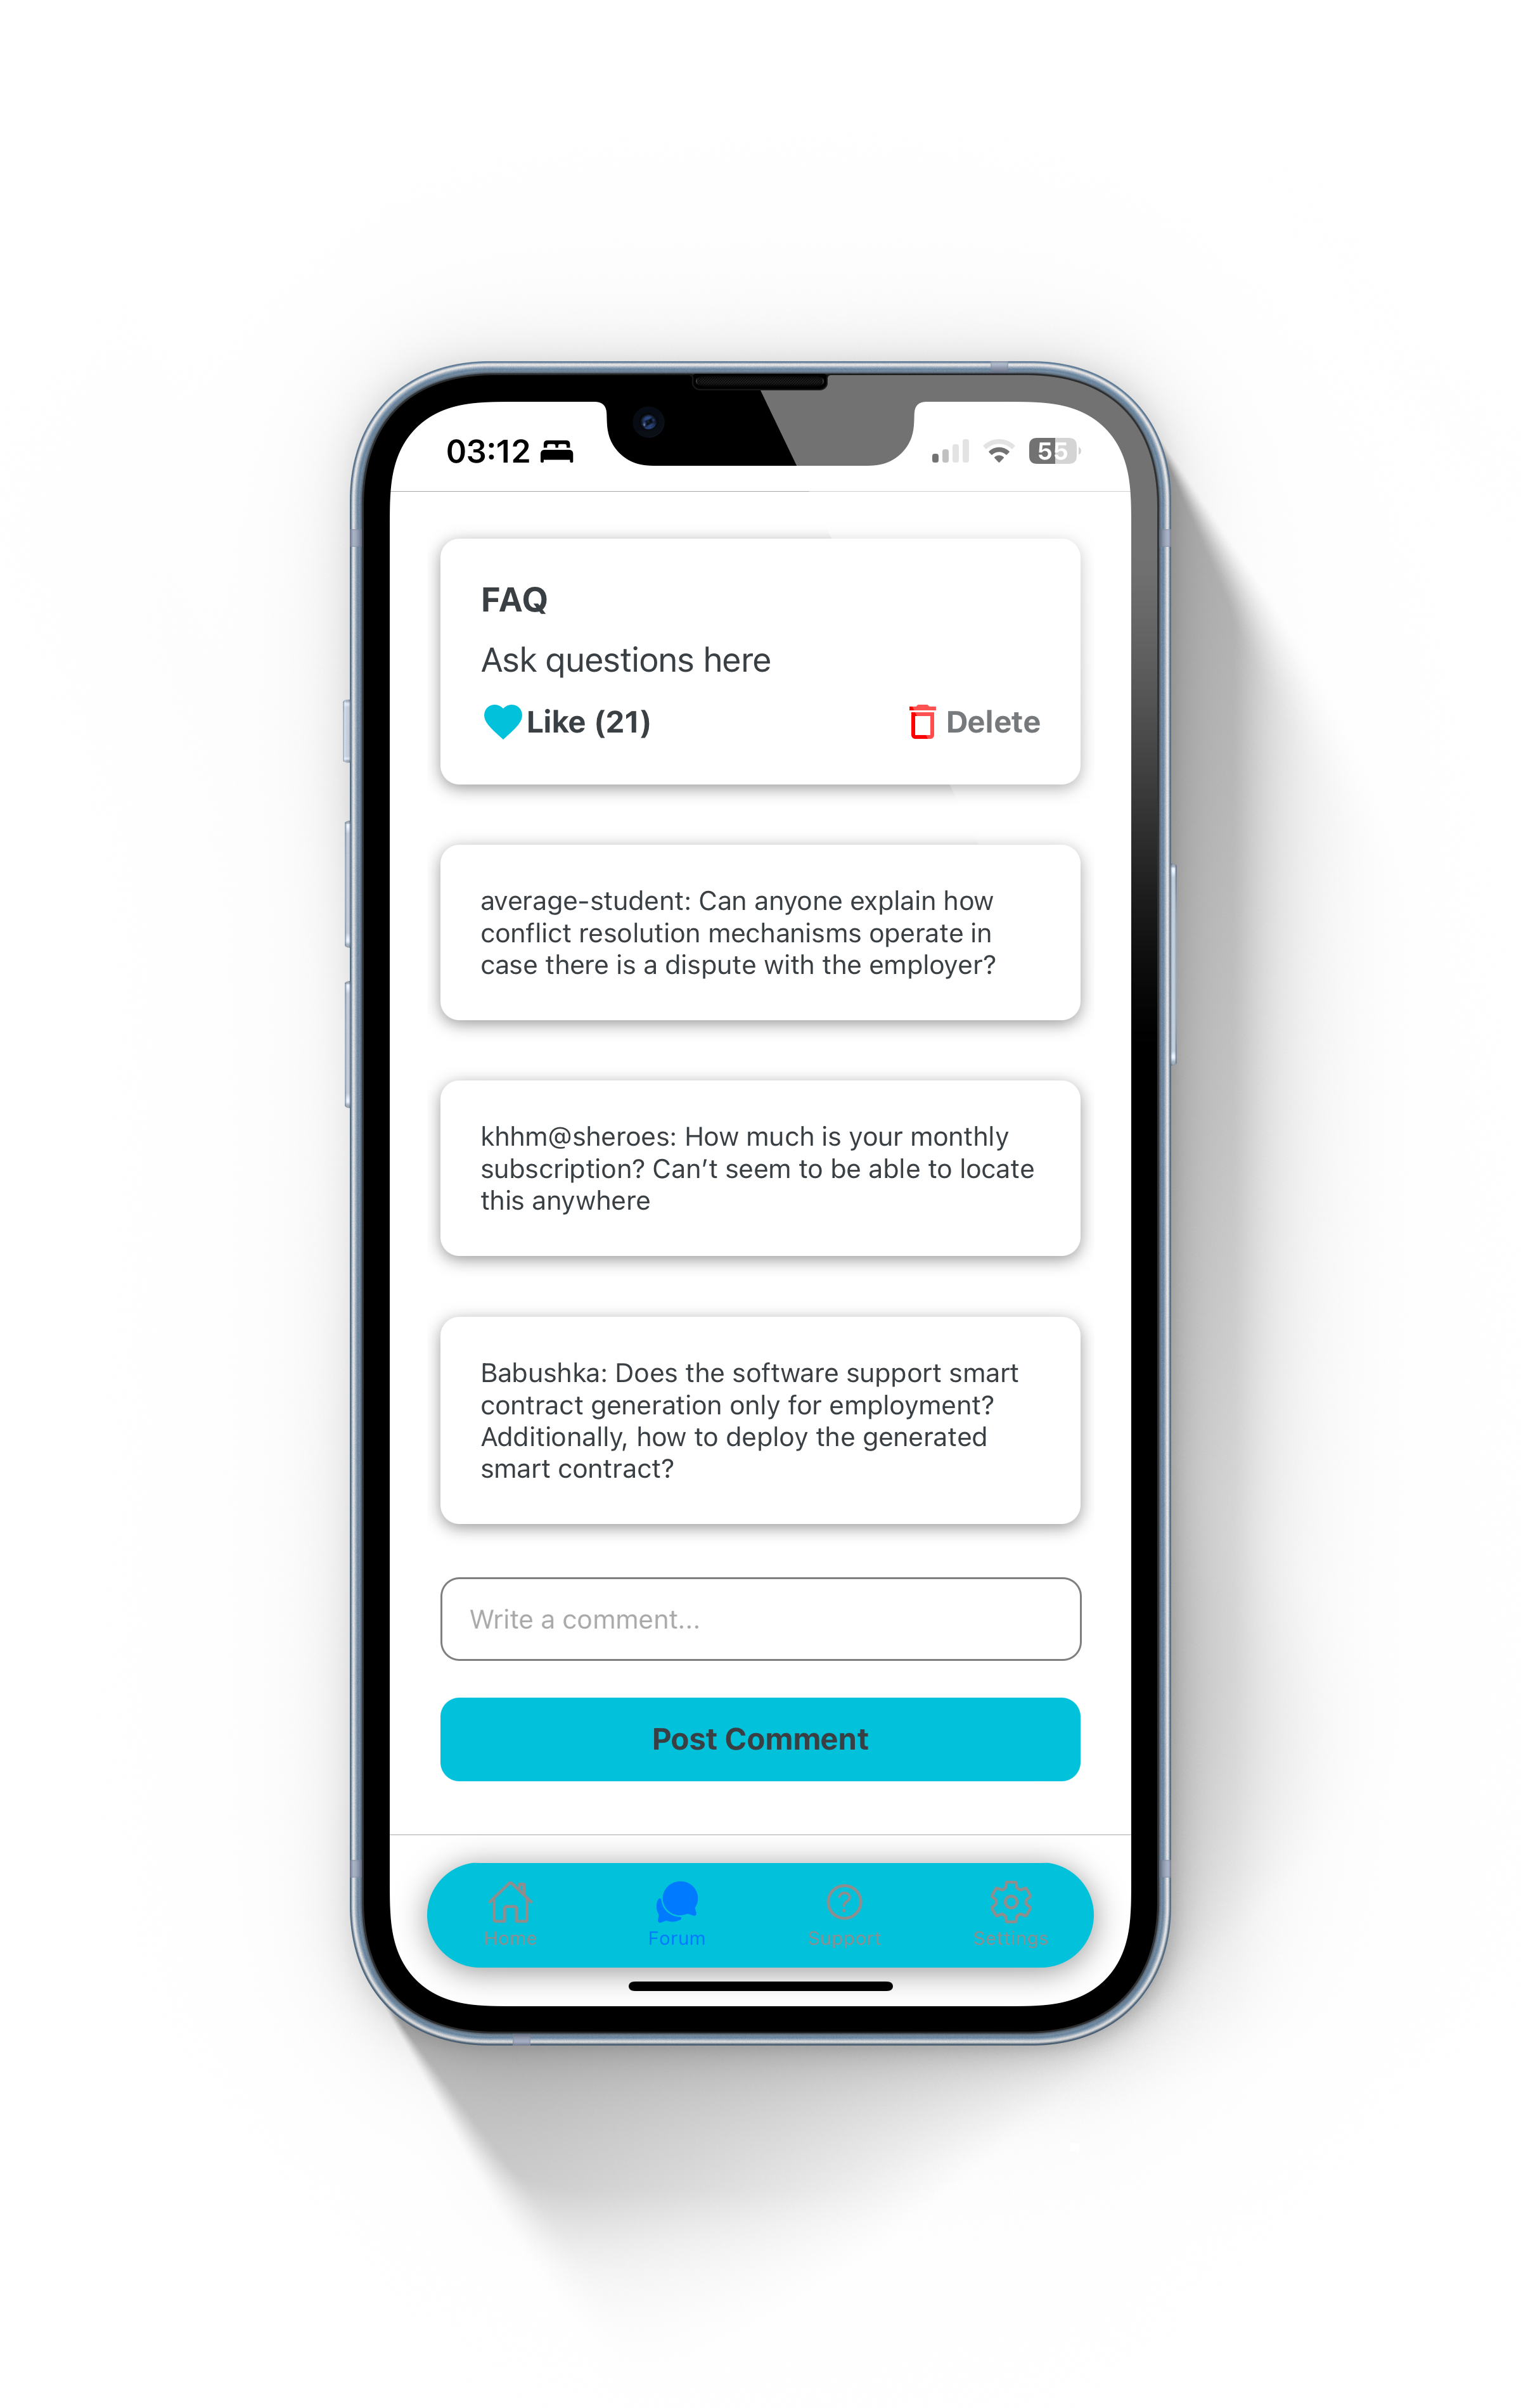
\includegraphics[width=0.43\textwidth]
    {LATEX/Appendices/Images/Software/Frontend/comment_screen.png}
    \label{fig:comment screen}
\end{figure}

\subsubsection{PostLoginScreens: UseCommentScreen.js}

The \texttt{UseCommentScreen.js} file defines a custom hook that manages the state and functionality of the comments screen.

\begin{itemize}
    \item \textbf{State Variables:}
    \begin{itemize}
        \item \texttt{comments}: An array to store the list of comments for the post.
        \item \texttt{newComment}: A string to store the content of a new comment.
    \end{itemize}

    \item \textbf{useEffect Hook for Fetching Comments:}
    \begin{itemize}
        \item The \texttt{useEffect} hook calls \texttt{fetchComments} to load the list of comments when the component mounts, updates, or when the post ID changes.
    \end{itemize}

    \item \textbf{Fetching Comments:}
    \begin{itemize}
        \item \texttt{fetchComments} is an asynchronous function.
        \begin{itemize}
            \item It makes a \texttt{GET} request to the backend to fetch the comments for the specified post.
            \item Updates the \texttt{comments} state with the fetched comments.
            \item Logs any errors encountered during the fetch.
        \end{itemize}
    \end{itemize}

    \item \textbf{Adding a Comment:}
    \begin{itemize}
        \item \texttt{handleAddComment} is an asynchronous function.
        \begin{itemize}
            \item It makes a \texttt{POST} request to the backend with the content of the new comment.
            \item If the request is successful, fetches the updated list of comments and updates the \texttt{comments} state using \texttt{LayoutAnimation} for a smooth transition.
            \item Logs any errors encountered during the comment addition.
        \end{itemize}
    \end{itemize}

    \item \textbf{Return Values:}
    \begin{itemize}
        \item The hook returns the \texttt{comments} array, \texttt{newComment} state, \texttt{setNewComment} function, \texttt{fetchComments} function, and \texttt{handleAddComment} function, which are used by the \texttt{CommentScreen} component to manage and display comments.
    \end{itemize}
\end{itemize}

\subsubsection{PostLoginScreens: SupportScreen.js}

The \texttt{SupportScreen.js} file defines a component responsible for providing a chat interface where users can interact with support agents.

\begin{itemize}
    \item \textbf{State Variables:}
    \begin{itemize}
        \item \textit{message}: A string to store the current user input message.
        \item \textit{messages}: An array to store the chat messages, initialised with a greeting message from the assistant.
    \end{itemize}

    \item \textbf{Sending Messages:}
    \begin{itemize}
        \item \textit{handleSendMessage} handles sending a message when the user presses the \textit{``send''} button.
        \begin{itemize}
            \item If the message is not empty, a new object is created with the user's input.
            \item The new message is added to the \textit{messages} array, and the input field is cleared.
        \end{itemize}
    \end{itemize}

    \item \textbf{Return Statement:}
    \begin{itemize}
        \item The component returns a \textit{View} container with the following elements:
        \begin{itemize}
            \item A header text displaying \textit{``Support Chat''}.
            \item A \textit{ScrollView} component to display the list of messages.
            \begin{itemize}
                \item Each message is rendered as a \textit{View} containing a \textit{Text} component with the message content.
                \item The message bubbles are styled differently based on whether the message is from an assistant or a user.
            \end{itemize}
            \item An input area at the bottom for the user to type and send messages.
            \begin{itemize}
                \item A \textit{TextInput} component for the user to type their message.
                \item A \textit{TouchableOpacity} button to send the message.
            \end{itemize}
            \item Multiple separator lines are included to enhance the visual layout.
        \end{itemize}
    \end{itemize}
\end{itemize}

\begin{figure}[!ht]
    \centering
    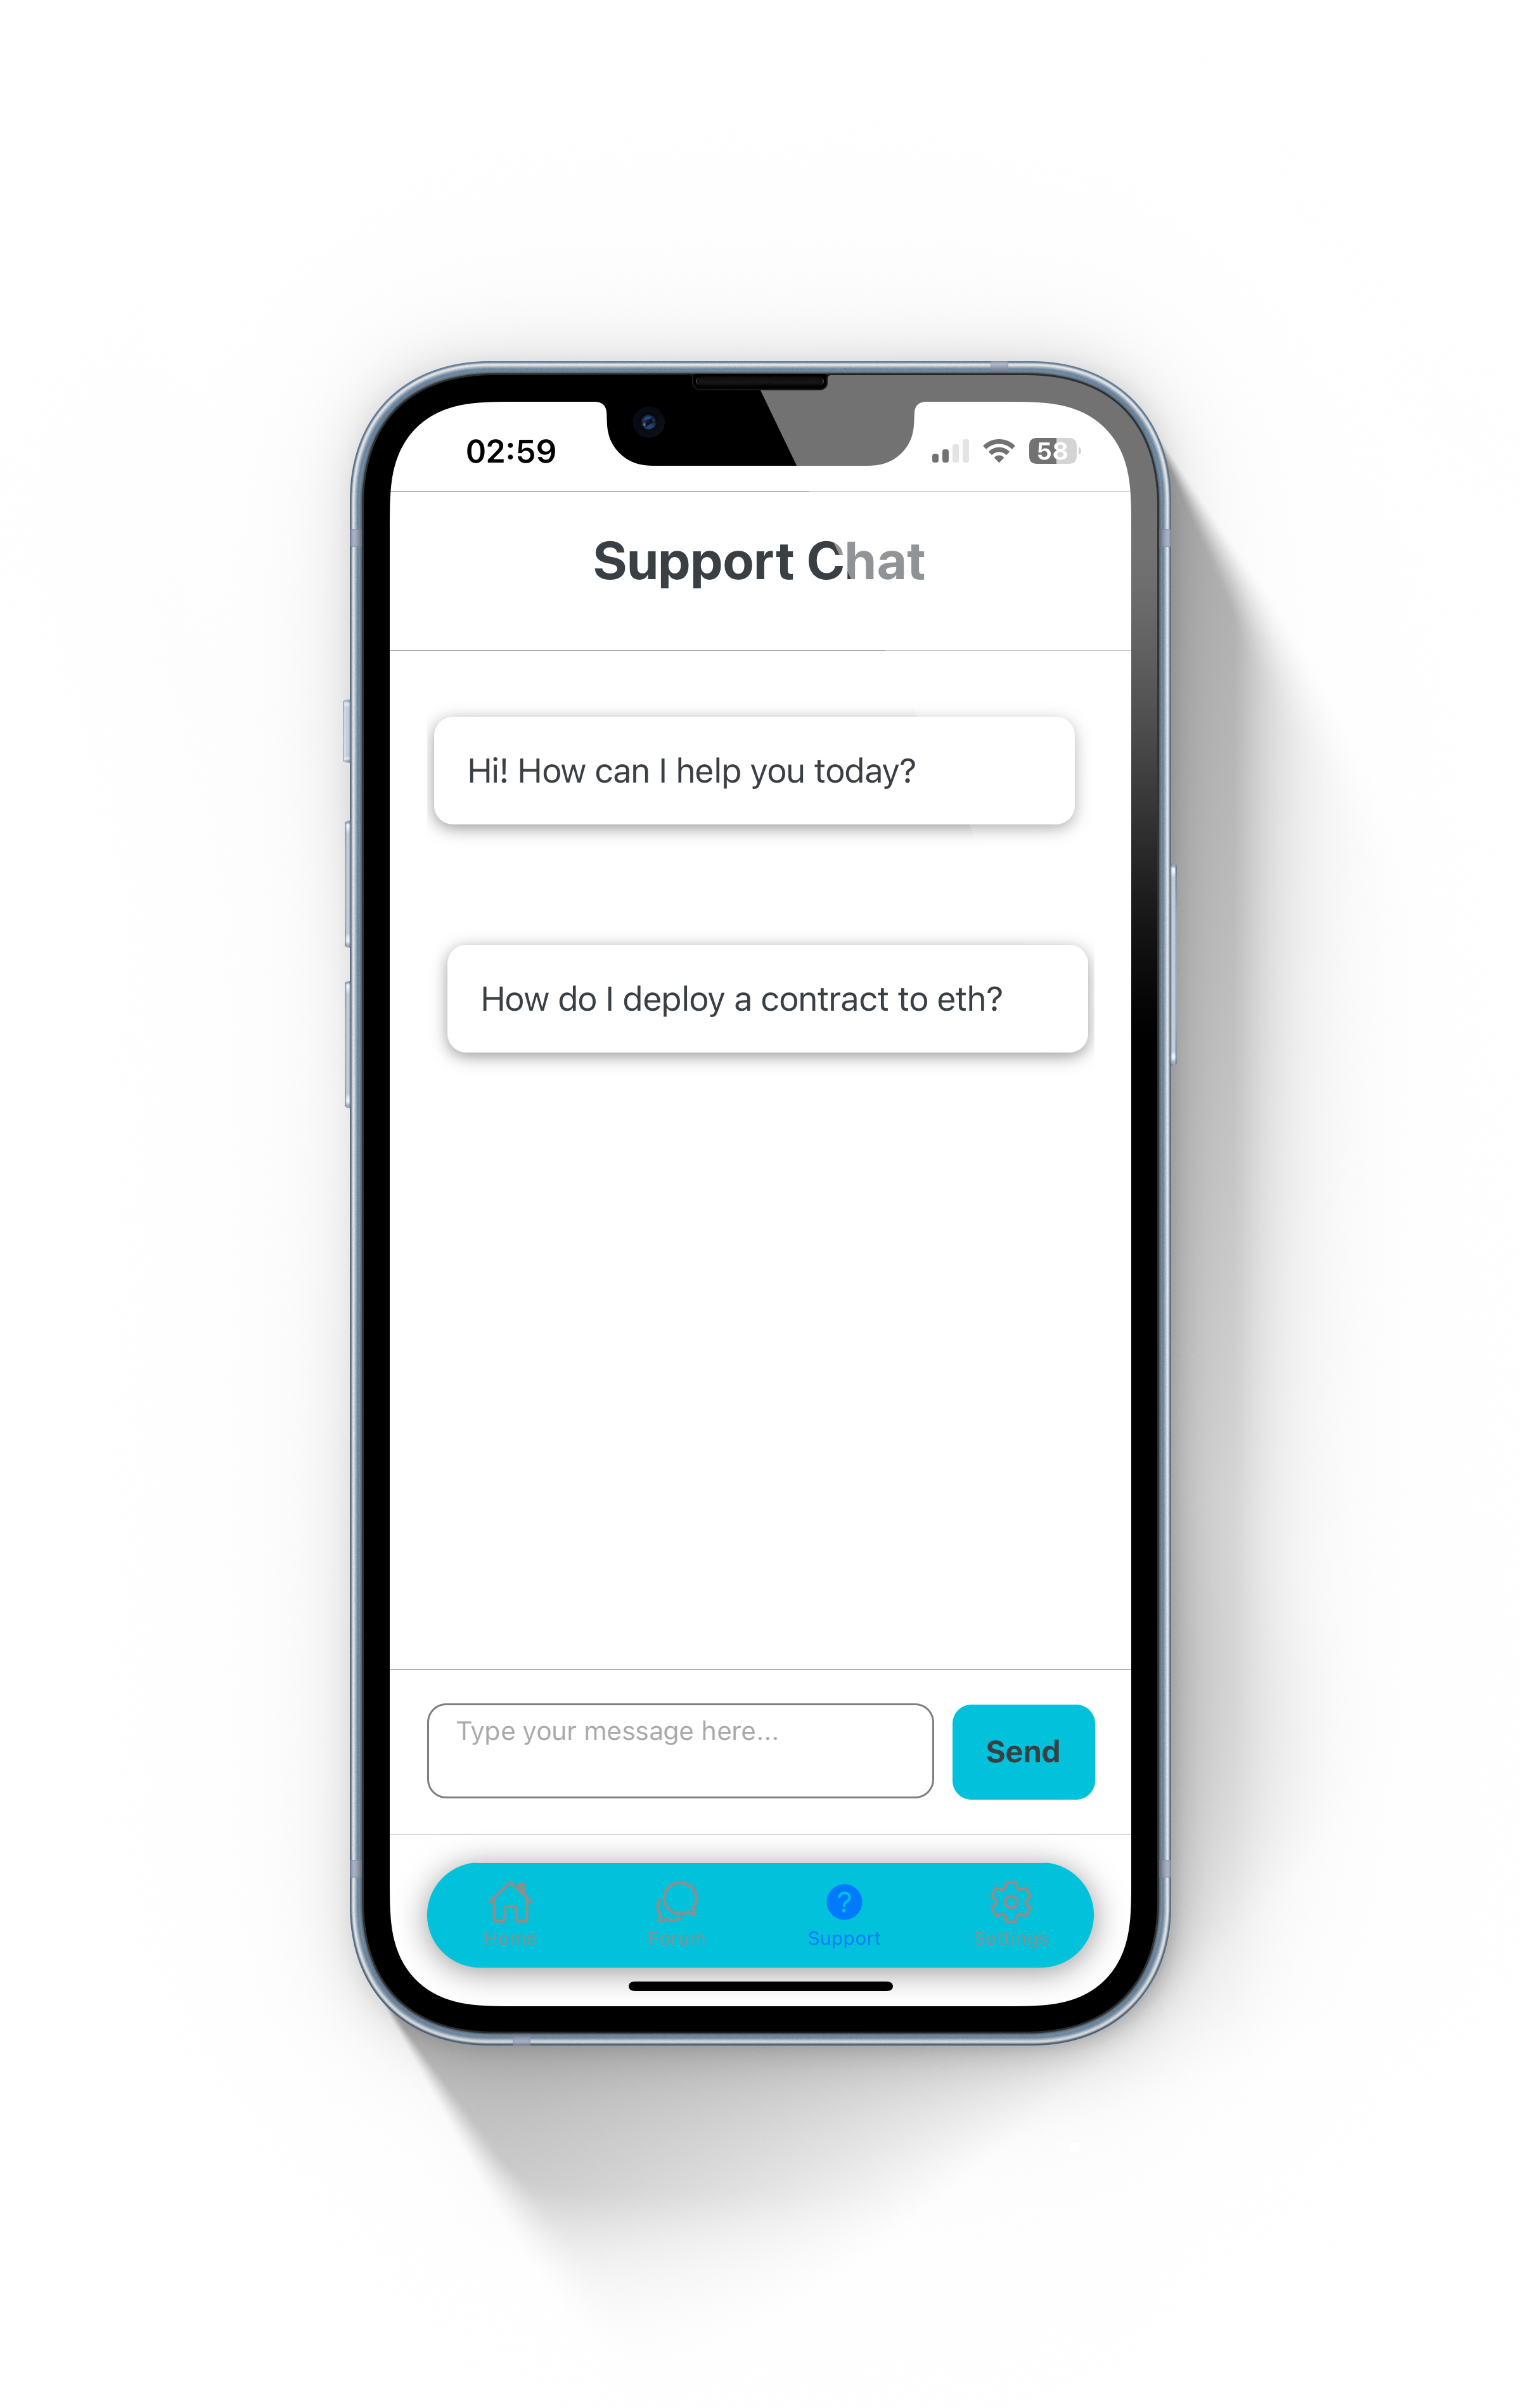
\includegraphics[width=0.43\textwidth]
    {LATEX/Appendices/Images/Software/Frontend/support_screen.png}
    \label{fig:support screen}
\end{figure}

Initially, it was planned to fine-tune another AI model to answer queries related to Solidity, smart contracts, and blockchain. However, due to time constraints, the AI model for this functionality was not developed. Additionally, the backend is not implemented to respond to these queries, resulting in a partially empty implementation. This functionality can be easily extended in future work.

\subsubsection{PostLoginScreens: SettingsScreen.js}

The \texttt{SettingsScreen.js} file defines a component responsible for providing a UI for adjusting application settings.

\begin{itemize}
    \item \textbf{Authentication and Notifications:}
    \begin{itemize}
        \item The \textit{handleLogout} function is obtained from \textit{AuthContext}.
        \item The \textit{notificationsEnabled}, \textit{setNotificationsEnabled}, and \textit{toggleNotifications} are obtained from and managed by \textit{useSettingsScreen}.
    \end{itemize}

    \item \textbf{Return Statement:}
    \begin{itemize}
        \item The component returns a \textit{View} container with the following elements:
        \begin{itemize}
            \item A header text displaying \textit{``Settings''}.
            \item A row container for toggling dark mode with \textit{Text} and \textit{Switch} components.
            \begin{itemize}
                \item The \textit{Switch} component toggles the \textit{isDarkMode} state using \textit{toggleTheme}.
            \end{itemize}
            \item A row container for toggling notifications with \textit{Text} and \textit{Switch} components.
            \begin{itemize}
                \item The \textit{Switch} component toggles the \textit{notificationsEnabled} state using \textit{toggleNotifications}.
            \end{itemize}
            \item A \textit{TouchableOpacity} button for logging out the user.
            \begin{itemize}
                \item This button triggers the \textit{handleLogout} function.
            \end{itemize}
            \item A separator line at the bottom for visual separation.
        \end{itemize}
    \end{itemize}
\end{itemize}

\begin{figure}[!ht]
    \centering
    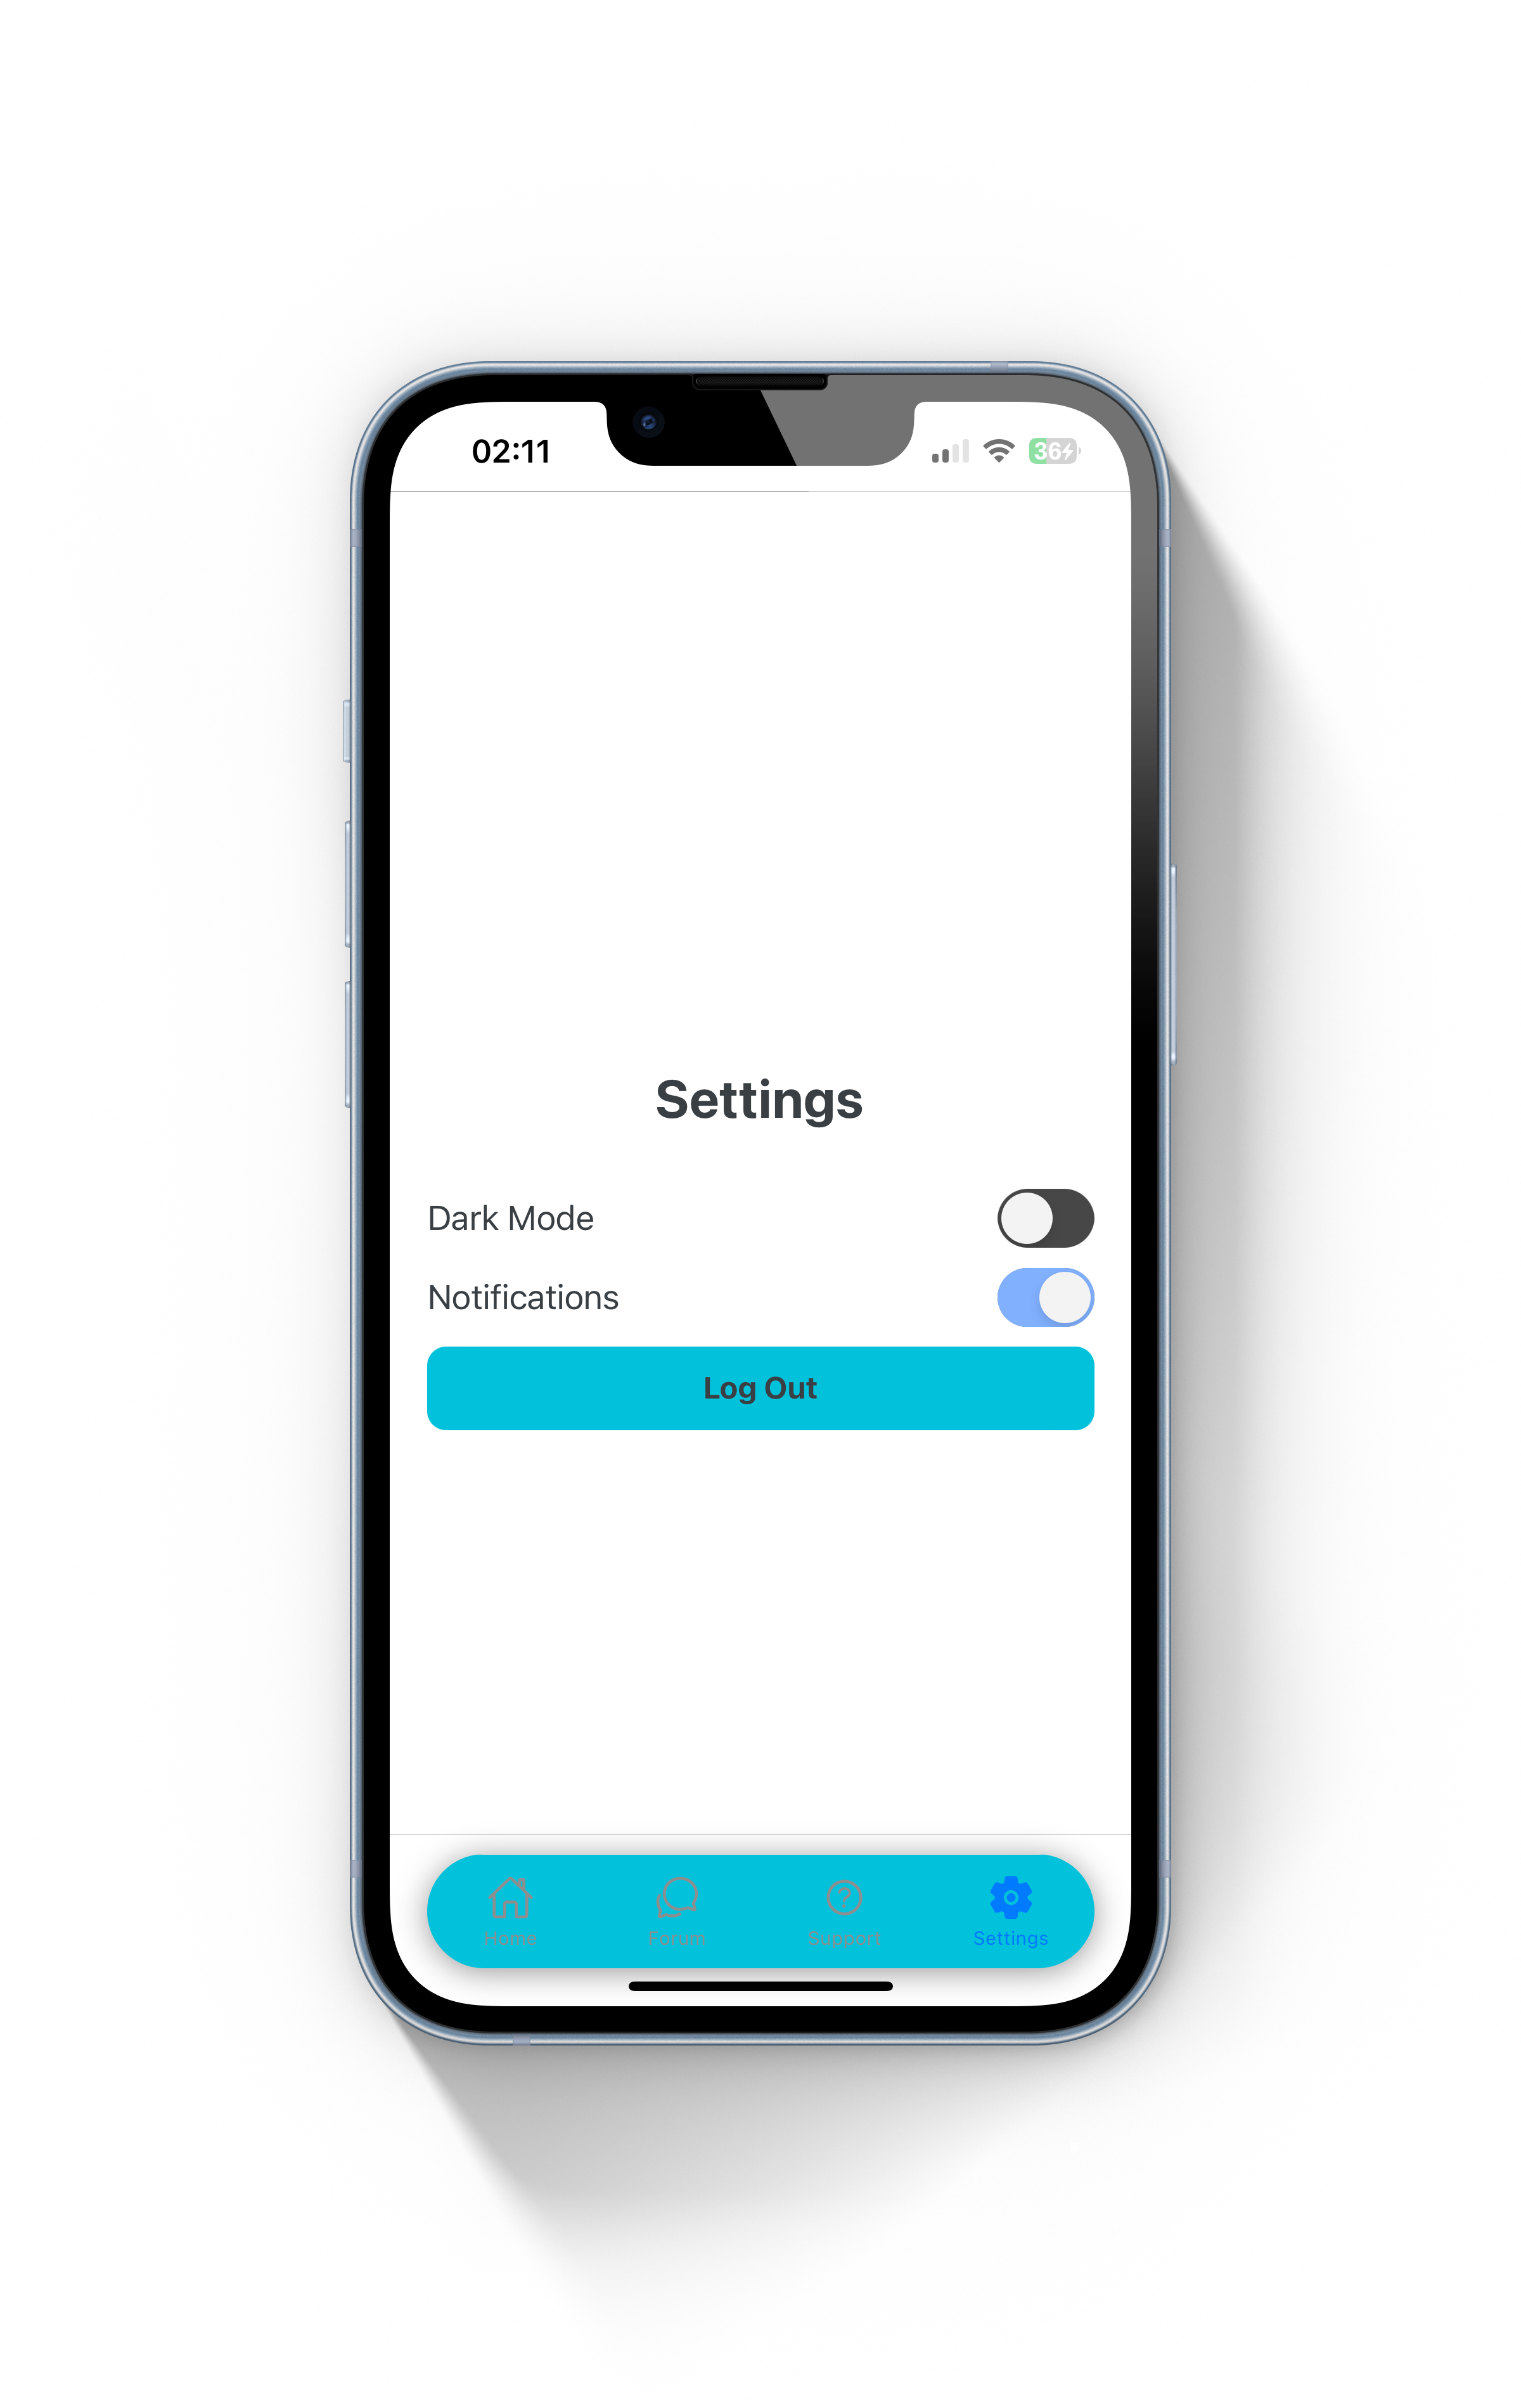
\includegraphics[width=0.43\textwidth]{LATEX/Appendices/Images/Software/Frontend/settings_screen.png}
    \label{fig:settings screen}
\end{figure}

\subsubsection{PostLoginScreens: UseSettingsScreen.js}

The \texttt{UseSettingsScreen.js} file defines a custom hook that manages the state and functionality of the settings screen.

\begin{itemize}
    \item \textbf{State Variables:}
    \begin{itemize}
        \item \textit{notificationsEnabled}: A boolean state variable to indicate whether notifications are enabled or disabled.
    \end{itemize}

    \item \textbf{useEffect Hook for Checking Notification Token:}
    \begin{itemize}
        \item The \textit{useEffect} hook runs a function \textit{checkNotificationToken} when the component mounts.
        \item \textit{checkNotificationToken} is an asynchronous function.
        \begin{itemize}
            \item It retrieves the token using \textit{SecureStore.getItemAsync}.
            \item Updates the \textit{notificationsEnabled} state to \textit{true} if a token is found, otherwise sets it to \textit{false}.
        \end{itemize}
    \end{itemize}

    \item \textbf{Toggling Notifications:}
    \begin{itemize}
        \item \textit{toggleNotifications} is an asynchronous function.
        \begin{itemize}
            \item It calculates and updates the notification status by negating the current \textit{notificationsEnabled} state.
            \item If notifications are being enabled, it calls \textit{savePushToken}.
            \item Otherwise, it calls \textit{deletePushToken}.
        \end{itemize}
    \end{itemize}

    \item \textbf{Return Values:}
    \begin{itemize}
        \item The hook returns the \textit{notificationsEnabled} state, \textit{setNotificationsEnabled} function, and \textit{toggleNotifications} function, which are used by the \textit{SettingsScreen} component to manage notification settings.
    \end{itemize}
\end{itemize}

\subsection{Cross-Platform Fixes}

Although React Native enables the use of a single codebase for both \textit{iOS} and \textit{Android} platforms, achieving a consistent appearance across these operating systems can be challenging. Native elements and behaviours are translated differently depending on the platform, which can lead to discrepancies in the app's appearance and functionality.

To address these differences, several strategies were employed, including the use of ternary operators to conditionally render components and apply specific styles for each platform. The following adjustments were made to the codebase:

\begin{itemize}
    \item \textbf{Keyboard Handling:} Keyboard height calculations differ between platforms, and scrolling adjustments were implemented to ensure that the focused input remains visible when the keyboard is active. 
    \item \textbf{Navigation Configuration:} The PostLoginTabs component employs platform-specific styling and behaviour. For example:
    \begin{itemize}
        \item The \textit{tabBarStyle} was adjusted using ternary operators to ensure that tab bar colors and shadows match the theme and look consistent across both platforms.
        \item The \textit{tabBarHideOnKeyboard} property was set to true on \textit{Android} to hide the tab bar when the keyboard is visible, a behaviour that differs from \textit{iOS}.
    \end{itemize}
    \item \textbf{Component Styling:} Various visual elements, such as icons, backgrounds, shadows, and animations, were conditionally styled due to differences in their rendering between \textit{iOS} and \textit{Android} platforms.
\end{itemize}

Despite these efforts, it is important to note that the application was primarily developed and tested on \textit{iOS}. While significant efforts were made to ensure a similar appearance on \textit{Android}, there may still be platform-specific bugs or visual inconsistencies.

\chapter{Legal, Social, Ethical and Professional Issues}

The usage of smart contracts for managing employment relations marks a significant technological leap. However, this approach poses certain professional concerns that must be properly addressed. 

\section{Relevant Professional Matters}

The relevant professional matters could be categorised into integrity, competence, confidentiality, and regulations compliance.

\subsection{Integrity and Honesty}

The fine-tuning of the custom AI model involves no real personal data. In order to not compromise any sensitive information, training datasets were created using fuzzing techniques and creative input. The capabilities and limitations of the platform are represented truthfully, avoiding overstatements about its efficacy or security. As stated in the evaluation chapter, the software is not yet ready for widespread adoption and requires further extensions. The inherent security problems associated with the use of current technology, such as smart contracts, are recognised. As cryptography specialist and lecturer at King's College London, Luca Vigano points out, "A computer is only truly safe when it is turned off and disconnected from all networks, hence any software poses a risk". Therefore although smart contract technology is improving, it is not immune to flaws. Despite being safer than many technologies established in the recent decades, smart contracts, like any other system based on blockchain technology, face potential vulnerabilities such as the 51\% attack. This type of attack enables entities with sufficient computational capacity to bypass network protection and completely rewrite the data saved in a distributed ledger. As with well-known and trusted systems such as \textit{OpenSSH}, new vulnerabilities are identified on a regular basis, necessitating constant vigilance. In the context of this project, although the technology itself offers greater security, it is still in its nascent stage and not yet suitable for production without further improvements in security measures. Nevertheless, the smart contracts have been developed to manage financial transactions and employment relations with the highest degree of transparency and security possible at this stage for a bachelor's thesis.

\subsection{Competence}

A high degree of competency must be maintained throughout software development processes. This necessitates ongoing learning and adaptation to new security mechanisms, as well as a grasp of the changing legal consequences of smart contract adoption. As previously indicated, this document serves as a bachelor's thesis and does not claim to offer the best solutions; the identified limitations are clearly outlined. Additionally, it has been noted that the author is a student, not an industry professional. Consistent with the evaluations detailed in the earlier chapters, a commitment to continuous learning is adhered to.

\subsection{Confidentiality}

Strict adherence to confidentiality agreements is demanded when handling sensitive employment data. To avoid unauthorised access, it must be encrypted and stored securely. Despite not deploying smart contracts within the scope of the application, the software is designed to prepare them for future deployment, which could expose private data. Addressing this will be a priority for future software extensions.

\subsection{Compliance with Regulatory Laws}

Blockchain's decentralised nature provides protection against forgeries, but it also serves as a double-edged sword; since data is immutable, any breach has long-term ramifications for privacy. The developed software partially adheres to international data protection standards, such as the \textit{GDPR} in the EU, which govern how personal data is acquired, stored, and shared. Specifically, no personal data is exposed to unauthorised individuals within the scope of the backend software. Additionally, appropriate permissions for data storage on the server are obtained from users. However, as soon as users deploy the generated smart contracts, their data becomes exposed to any node within the deployed blockchain. 
    
In terms of employment Laws, the developed smart contracts were designed to comply with international ones, but there are inherent restrictions to their area of coverage, particularly in terms of minimum wage and overtime work. Limitations arise primarily because the AI model only serves to translate legal employment contracts into code. This, in turn, implies no control over the original data input, which may include salaries below the minimum wage requirement. Furthermore, the absence of a specific job performance metrics evaluation system causes concerns, as the software does not address overtime workload issues, potentially leading to non-compliance with employment standards.
    
Regarding intellectual property rights, throughout the training of the AI model, those of \textit{OpenAI} and others are respected so that the use external technology does not infringe upon the copyrights of others. Additionally, the legitimate rights of other third-party tools used during development are properly credited and utilised in accordance with their licensing agreements.

\section{Environmental Impact}

\paragraph{Negative Impacts}

Traditional blockchain systems, especially those that rely on proof-of-work mechanisms, are renowned for their high energy consumption. The mining process requires substantial computational power, which implies the usage of significant amounts of electricity. This substantial energy consumption contributes to increased carbon emissions, which is concerning in light of global climate change. Furthermore, the hardware-intensive computations required to validate smart contract states in the blockchain necessitate servers that often have short lifespans due to continuous operation, contributing to electronic waste.

\paragraph{Indirect Positive Impacts}

This software, by digitising contract management and execution, can reduce the dependency on paper, minimising deforestation and waste associated with paper manufacture and disposal. Additionally, as it automates some business processes, this can potentially reduce the need for physical transport and office spaces, thus lowering overall energy consumption and gas emissions.

\section{Social and Ethical Implications}

Given the experimental nature of the software, the likelihood of market adoption is extremely low at this stage. However, ethical reasons justify and require a hypothetical study of its potential consequences.

The automation of contract management and performance evaluation may minimise human control in HR operations, posing a risk of job displacement. Consequently, this leads to justified concerns about the dehumanisation of workplace relationships. Although the software was designed to automate manual workloads and provide better social security, unintended negative outcomes may still occur. Ethical considerations must address how society will manage the transition for workers who may lose their jobs to automation.

\section{Public Well-Being Impact}

The project promotes equal access to IT benefits by making the software accessible to a wide demographic, regardless of belief, race, disability, gender, or any other protected characteristics. Actions are taken in the public interest, maintaining transparency about the experimental nature of smart contracts and their legal recognition. Smart contracts can make employment contracts more accessible to a wider range of people, especially those in distant or underserved places, by eliminating the need for middlemen and lowering entry barriers. With transparent and enforceable contracts, employees can experience greater job security and clarity regarding employment terms, contributing to social stability. Additionally, the technology can help protect workers from exploitative practices by strictly enforcing the terms of employment, provided those terms are fairly applied and once the software is complete.

\section{Sustainability, Economic, and Commercial Factors}

By automating contract enforcement and management, smart contracts can enhance the long-term viability of enterprises by reducing operational risks and costs. The automation of contract execution through these technologies significantly lowers expenses associated with legal services, administrative processing, and dispute resolution. Furthermore, smart contracts enable businesses to function more efficiently across borders, allowing for market expansion and access to global talent pools without incurring the significant costs that are traditionally associated with such growth.

The distinct characteristics of smart contract technology also attract venture capitalists interested in technology-driven company models, stimulating economic growth. Furthermore, the capacity to automate and protect employment contracts can lead to the development of new business models, such as decentralised autonomous organisations or blockchain-based gig economy platforms.

However, as previously mentioned, the technology challenges traditional employment structures, potentially displacing administrative jobs, necessitating careful assessment of the broader employment impact.

\chapter{Results, Analysis, and Evaluation}

\section{Software Testing}

\subsection{Backend Testing}

The \textit{AI-Chain-Contracts} project adopts a strong testing plan to ensure the reliability of each component within its application. The tests are based on \texttt{Django's testing framework}, with extra help from \texttt{Pytest}. Every application of the backend project, whether \textit{Forums}, \textit{Contracts}, \textit{Accounts}, or \textit{Notifications}, includes a directory called \textit{``tests''} containing test files corresponding to each module written. To make tests predictable and separate them from outside services, such as sending notifications or interacting with the AI model, \textit{unittest.mock} library is utilised.

The \texttt{pytest.ini} configuration file sets up the testing environment through the following flags:

\begin{itemize}
    \item \textbf{``DJANGO\_SETTINGS\_MODULE''}: Set to \textit{AIChainContracts.settings} for correct context during test runs.
    \item \textbf{``asyncio\_mode''}: Set to \textit{auto} to enable asynchronous input and output operations.
    \item \textbf{``addopts''}: Includes options like \textit{``--nomigrations''} to disable migrations for faster test execution, \textit{``--cov=.''} for enabling coverage measurements, and \textit{``-cov-report=term-missing''} for terminal coverage reports.
    \item \textbf{``python\_files''}: Specifies test file recognition patterns: their names are either \textit{``tests.py''}, they start with \textit{``test\_*''}, or end with \textit{``*\_tests.py''}. 
    \item \textbf{``testpaths''}: Specifies directories for \textit{pytest} to find test files.
    \item \textbf{``norecursedirs''}: Lists directories to ignore during test search, including hidden directories, \textit{venv}, \textit{sdist}, \textit{build}, \textit{node modules}, and \textit{Django} migration files.
    \item \textbf{``.coveragerc''}: Configures coverage reporting.
\end{itemize}

\subsubsection{Testing ASGI and WSGI Configurations}

Tests for synchronous and asynchronous requests are found in \textit{test\_wsgi.py} and \textit{test\_asgi.py} files. These tests ensure proper configuration of \textit{WSGI} and \textit{ASGI} applications to handle WebSocket and HTTP traffic. The middleware stack and routing protocols are also verified.

\subsubsection{Testing Settings}

In \textit{test\_settings.py}, the configuration tests confirm that database settings, middleware, and installed apps are applied correctly for different environments (development, testing, production). Additionally, authentication methods and CORS headers are also checked for security purposes. 

\subsubsection{Testing Admin Interfaces}

Admin tests, as shown in each testing subdirectory of every application within the \textit{test\_admin.py} files, verify that models are correctly registered with Django's admin. Alongside, they also check if admin pages render accurately (this includes list and detail views). This testing often involves using \textit{RequestFactory} to simulate admin interface requests.

\subsubsection{Testing Application Configuration}

Application configuration tests, located in files named \textit{test\_apps.py}, verify that Django applications are correctly initialised.

\subsubsection{Testing Models}

In each \textit{``tests''} subdirectory of each application, there is a file named \textit{test\_models.py}. These files typically contain test cases that validate the business logic embedded in the models, relationships, and custom methods. The Django \textit{TestCase} class is used extensively for database interaction, utilising Django's database rollback functionalities to ensure test isolation.

Model testing involves:
\begin{itemize}
    \item Validating model fields and attributes.
    \item Checking model methods for expected behavior.
    \item Ensuring the integrity of relationships between models.
\end{itemize}

\subsubsection{Testing Serialisers}

Serialisers are tested to ensure that they accurately serialise and deserialise data. These tests, located in each subdirectory of each application under \texttt{test\_serialisers.py}, check:
\begin{itemize}
    \item Field validation.
    \item Output data structure.
    \item Integration with models for creating and updating records.
\end{itemize}

\subsubsection{Testing URL Routing}

Routing tests in each subdirectory of each application in files named \textit{test\_urls.py} verify that URLs correctly map to views. The tests utilise Django's \textit{resolve} and \textit{reverse} functions to simulate web requests and ensure endpoints are accessible.

\subsubsection{Testing Validators}

In the \textit{test\_validators.py} file, tests ensure that custom validation logic in models or serialisers behaves as expected. These tests:

\begin{itemize}
    \item Validate input data for compliance with defined rules, ensuring data integrity.
    \item Use Python's built-in \texttt{ValidationError} to ensure that invalid data is caught and handled properly.
\end{itemize}

\subsubsection{Testing Views}

View tests in \textit{test\_views.py} files ensure HTTP interfaces function as expected, checking response status codes, data structure, and handling of authentication and permissions. Mocking is extensively used to isolate view tests from external dependencies.

\subsubsection{Testing Consumers}

Testing \textit{WebSocket} consumers, as outlined in \texttt{test\_consumers.py}, includes:

\begin{itemize}
    \item Using the \texttt{WebsocketCommunicator} to simulate web socket interactions, testing both the connection lifecycle and message handling.
    \item Ensuring that messages sent over web sockets are received and broadcast correctly to all connected clients, using Django Channels' groups and messaging layers.
\end{itemize}

\subsubsection{Testing Routing}

Routing tests for web sockets ensure that the \texttt{WebSocket} URLs are correctly configured to handle incoming connections, as shown in \texttt{test\_routing.py}.

\subsubsection{Testing Utility Functions}

Utility function tests in \textit{test\_utils.py} focus on external integrations and side effects such as sending notifications. These tests:

\begin{itemize}
    \item Often use mocking to simulate external services and verify that utilities behave correctly under different scenarios without sending actual requests.
    \item Check that the functions handle errors correctly and perform their intended side effects.
\end{itemize}

\subsubsection{Coverage}

Comprehensive testing is one of the most important aspects of maintaining software reliability. Hence, by achieving a 100\% coverage combined with continuous integration, the backend achieves stability and dependability.

\begin{figure}[!ht]
    \centering
    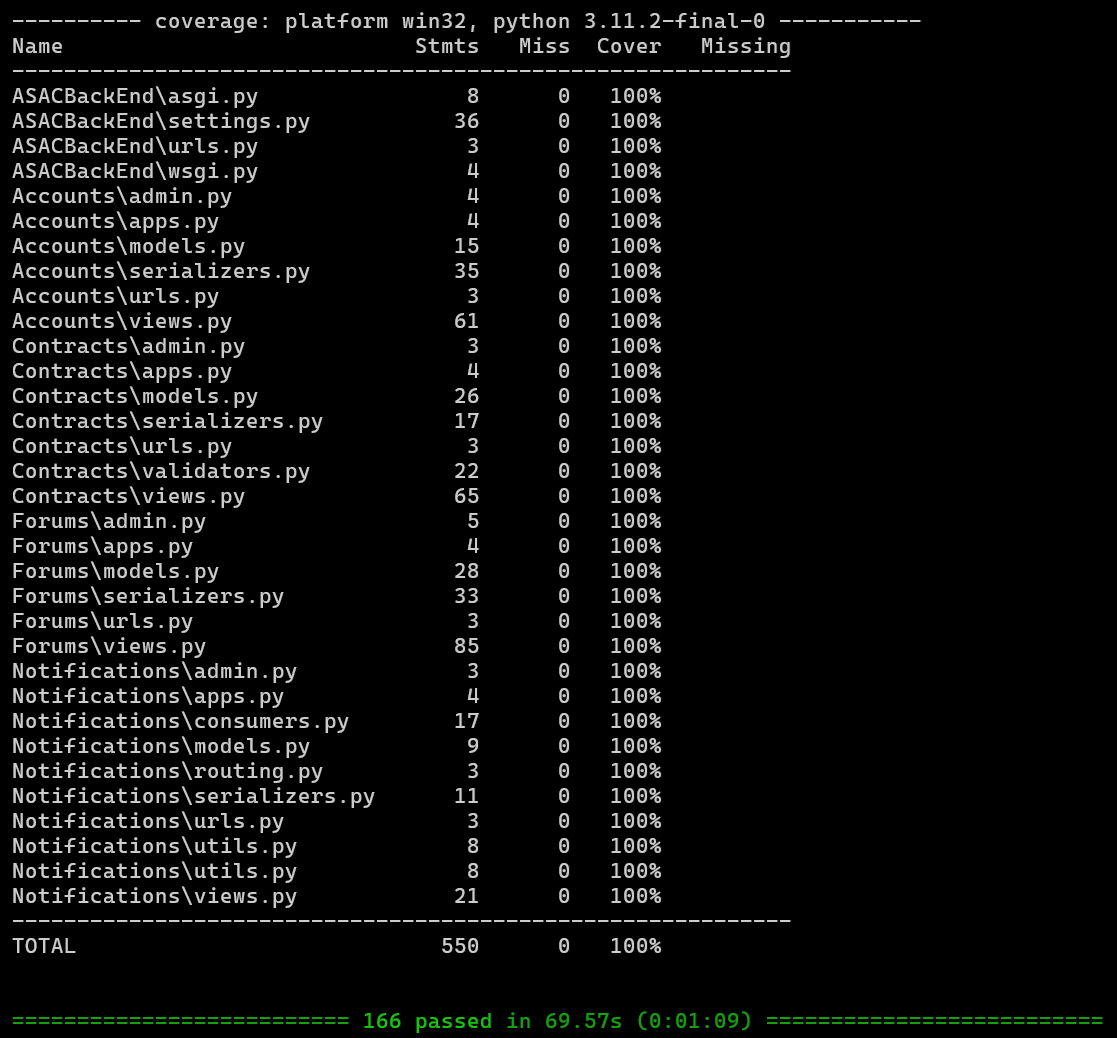
\includegraphics[width=1\textwidth]
    {LATEX/Appendices/Images/Software/Backend/backend_testing_report.png}
    \caption{Backend Test Coverage Report}
    \label{fig:backend_testing}
\end{figure}

\subsection{Frontend Testing}

The \texttt{\_\_tests\_\_} folder in the root directory of the UI contains the test files for the application. Each test file is stored in a structure that mirrors the corresponding file in the root directory and is named similarly but with \texttt{.test.js} at the end. The configuration for testing is set up as follows in the \texttt{package.json} file:

\begin{itemize}
    \item \textbf{Jest Configuration}: For compatibility with Expo, \textit{``preset''} is set to \textit{jest-expo}. \textit{JavaScript} and \textit{TypeScript} files are transformed using \textit{babel-jest} specified under the \textit{``transform''} parameter. Coverage data is gathered from designated files specified in \textit{``collectCoverageFrom''} and is enabled with \textit{``collectCoverage''}. The output format of coverage reports is defined in \textit{``coverageReporters''}, and strict coverage thresholds are set through \textit{``coverageThreshold''} to 100\% for branches, functions, lines, and statements. Module handling is managed by \textit{``moduleFileExtensions''} for file extensions, \textit{transformIgnorePatterns''} for excluding modules during transformation, and \textit{``setupFilesAfterEnv''} configures \textit{@testing-library/jest-native/extend-expect} for post-environment setup.
\end{itemize}

\paragraph{Additional Information}

This section summarises the recurring elements used across all test suites. To avoid redundancy, these details will not be reiterated in the future.

\begin{itemize}
    \item \textbf{Setup Configuration:} Tests use Jest and the React Native Testing Library.
    \item \textbf{Imports and Mock Implementations:}
    \begin{itemize}
        \item Essential imports typically include \textit{React}, \textit{react-native}, \textit{@react-navigation/native}, and \textit{render} from \textit{@testing-library/react-native}.
        \item Each test file has its own set of customised mocks, which usually cover modules such as \textit{expo-notifications}, \textit{@react-navigation}, \textit{expo-file-system}, \textit{AppNavigator}, \textit{ErrorBoundary}, \textit{Authentication}, \textit{Keyboard}, \textit{Theme}, and custom hooks used to control the screens.
    \end{itemize}
    \item \textbf{Test Suites:}
    \begin{itemize}
        \item Are defined with \texttt{describe(``<Name of the original application>'', ...)} and contain multiple test cases.
        \item \texttt{beforeEach} and \texttt{afterEach} blocks are used to set up and then clear mocks to achieve a clean environment for each test.
    \end{itemize}
    \item \textbf{General Tests Execution:}
    \begin{itemize}
        \item \textbf{Environment:} Each component is tested within its respective provider environment to simulate real application conditions.
        \item \textbf{Methodology:} Makes considerable use of assertions to confirm anticipated results while simulating external dependencies with the help of mocks, ensuring test isolation.
        \item \textbf{Cleanup:} Ensures that mocks are cleared and functions restored post-testing to prevent test contamination.
    \end{itemize}
\end{itemize}

\subsubsection{Testing Root Directory}

\begin{itemize}
    \item \textbf{App.test.js:}
    \begin{itemize}
        \item These tests aim to confirm that the main application component properly integrates its submodules while managing notifications and global settings.
        \item The setup includes \textit{expo-notifications}, \textit{AppNavigator}, \textit{ErrorBoundary}, and other necessary modules.
        \item \textbf{Core Tests:}
        \begin{itemize}
            \item \textbf{Platform Specific Behaviour}: Checks whether \textit{Android} devices have layout animation turned on.
            \item \textbf{Error Handling}: Ensures that the global error handler is configured correctly in development mode and accurately logs errors.
            \item \textbf{Notification Management}: Tests handling of notifications, ensuring correct configuration and cleanup of notification listeners.
            \item \textbf{Component Rendering}: Verifies that the \textit{AppNavigator} is included as a child component in order to ensure that the app is rendering correctly.
        \end{itemize}
    \end{itemize}

    \item \textbf{babel.config.test.js:}
    \begin{itemize}
        \item The objective of this test suite is to verify the correct loading of Babel configurations based on different environment settings.
        \item There is a helper function that uses \textit{loadConfig(envSetting)} to simulate configuration loading.
        \item \textbf{Core Tests:}
        \begin{itemize}
            \item \textbf{Environment Configurations:} Checks configuration correctness for default, test, and production environments by verifying the appropriate inclusion of presets and plugins.
        \end{itemize}
    \end{itemize}

    \item \textbf{ErrorBoundary.test.js:}
    \begin{itemize}
        \item The goal of this test suite is to evaluate the \textit{ErrorBoundary's} capacity to catch and handle errors from child components.
        \item The setup utilises a \textit{ProblemChild} component that simulates error scenarios.
        \item \textbf{Core Tests:}
        \begin{itemize}
            \item \textbf{Error Catching}: Tests error catching from child components and verifies logging.
            \item \textbf{Fallback UI}: Checks the display of fallback UI upon error detection.
            \item \textbf{Normal Rendering}: Ensures normal rendering behaviour when no errors are present.
        \end{itemize}
    \end{itemize}
\end{itemize}

\subsubsection{Testing Components Directory}

\begin{itemize}
    \item \textbf{Common Patterns}: Each test involves using mocks for \textit{expo-secure-store}, \textit{global.fetch}, and \textit{WebSocket} to simulate external interactions.

    \item \textbf{Authentication.test.js:}
    \begin{itemize}
        \item \textbf{Objective:} Ensures authentication module works properly.
        \item \textbf{Setup and Mocks:} Uses mocks for \textit{expo-secure-store}, \textit{global.fetch}, and \textit{WebSocket} to simulate external interactions.
        \item \textbf{Core Tests:}
        \begin{itemize}
            \item \textbf{Token Validation:} Verifies that the token validation process correctly identifies valid and invalid tokens and handles network errors appropriately.
            \item \textbf{Sign Up:} Tests cover user registration scenarios, including missing fields, password mismatches, and server error responses.
            \item \textbf{Login and Logout Processes:} Tests check how tokens are managed and how errors are communicated to the user.
        \end{itemize}
    \end{itemize}

    \item \textbf{Keyboard.test.js:}
    \begin{itemize}
        \item \textbf{Objective:} Evaluates the \textit{KeyboardProvider's} ability to manage keyboard visibility during text input interactions.
        \item \textbf{Setup and Mocks:} Mocks \textit{Keyboard}, \textit{Dimensions}, and \textit{TextInput} to control keyboard and screen interactions.
        \item \textbf{Core Tests:}
        \begin{itemize}
            \item \textbf{Keyboard Visibility:} Ensures that keyboard visibility state updates correctly in response to show and hide events, with implementations varying between \textit{iOS} and \textit{Android} platforms.
            \item \textbf{Reference Registration:} Tests the proper registration and unregistration of scroll view and text input references, assessing cleanup on component unmount.
            \item \textbf{Interaction with TextInput:} To make sure that input fields are not obscured by the keyboard, this test examines how the UI adjusts the view when a text input is focused.
        \end{itemize}
    \end{itemize}

    \item \textbf{Notifications.test.js:}
    \begin{itemize}
        \item \textbf{Objective:} Tests the reliability of \textit{WebSocket} connections and the scheduling of push notifications.
        \item \textbf{Setup and Mocks:} Involves mocking \textit{expo-secure-store}, \textit{expo-notifications}, \textit{global.fetch}, and \textit{WebSocket}.
        \item \textbf{Core Tests:}
        \begin{itemize}
            \item \textbf{WebSocket Management:} Verifies the correct opening and closing of web socket connections, including error handling.
            \item \textbf{Notification Handling:} Focuses on how incoming messages trigger notification scheduling and how token management operations handle errors.
            \item \textbf{Integration and Context Provision:} Checks for the maintenance of functional integrity by making sure that the web socket context is correctly provided to child components.
        \end{itemize}
    \end{itemize}

    \item \textbf{Theme.test.js:}
    \begin{itemize}
        \item \textbf{Objective:} Tests the theme management functionality.
        \item \textbf{Setup and Mocks:} Mocks \textit{expo-secure-store} for simulating theme storage operations.
        \item \textbf{Core Tests:}
        \begin{itemize}
            \item \textbf{Default Theme Settings:} Confirms that the default ``light'' theme is correctly set upon initialisation.
            \item \textbf{Theme Initialisation:} Checks the retrieval and setting of the theme from storage at startup.
            \item \textbf{Theme Toggling:} Verifies that the ``light'' and ``dark'' theme toggles are applied successfully and that the preferences are saved.
            \item \textbf{Dark Mode Detection:} Verifies that the application accurately detects the dark mode setting based on the stored theme preference.
        \end{itemize}
    \end{itemize}
\end{itemize}

\subsubsection{Testing Navigation Directory}

\begin{itemize}
    \item \textbf{AppNavigator.test.js:}
    \begin{itemize}
        \item Using mocked contexts for authentication and theme, tests verify that the \textit{AppNavigator} correctly renders navigation stacks based on the user's authentication status.
        \item \textbf{Core Tests:}
        \begin{itemize}
            \item Verification of \textit{PostLoginTabs} rendering when a user is authenticated.
            \item Verification of \textit{PreLoginStack} rendering when a user is unauthenticated.
        \end{itemize}
    \end{itemize}

    \item \textbf{PreLoginStack.test.js:}
    \begin{itemize}
        \item Concentrates on checking the correct rendering of screens within the \textit{PreLoginStack} through verifying the accessibility of all navigation screens for unauthenticated users via navigation simulations.
    \end{itemize}

    \item \textbf{PostLoginTabs.test.js:}
    \begin{itemize}
        \item Tests the \textit{PostLoginTabs} for correct rendering of tabs.
        \item \textbf{Core Tests:}
        \begin{itemize}
            \item Verification of tab functionality and correct rendering of associated stacks, including navigation simulations.
            \item Theme-specific rendering checks to ensure both light and dark modes are correctly applied.
        \end{itemize}
    \end{itemize}
    
    \item \textbf{Debugging and Resolution:}
    \begin{itemize}
        \item Initially, tests were failing because of issues related to the \textit{SafeAreaProvider} wrapping the entire navigation structure. The screen and all components below it were not rendering correctly, leading to empty debug outputs. After numerous failed attempts to troubleshoot, extensive research was conducted. It was found that mocking the \textit{SafeAreaContext} and its related hooks resolved the issue \cite{StackOverflowSafeAreaContextIssue2021, GithubSafeAreaContextIssue2019}.
        \item This emphasises how important it is to mock environmental components correctly in Jest, which can often be under-documented.
    \end{itemize}
\end{itemize}

\subsubsection{Testing Styles Directory}

All style sheets are subjected to unit testing under the \textit{``styles''} directory. The strategy involved rendering and asserting the styles for both light and dark themes, as well as for \textit{iOS} and \textit{Android}, since the stylings vary slightly due to differences in the rendering of some elements between the platforms. Objectively speaking, this was the simplest aspect of UI testing so far. The directory includes the following test files:

\begin{enumerate}
    \item \textit{ThemeStyles.test.js}
    \item \textit{GloballySharedStyles.test.js}
    \item \textit{LocallySharedStylesPreLoginScreens.test.js}
    \item \textit{LocallySharedStylesHomeScreens.test.js}
    \item \textit{LocallySharedStylesForumScreens.test.js}
    \item \textit{LocallySharedStylesSupportScreens.test.js}
    \item \textit{LocallySharedStylesSettingsScreens.test.js}
\end{enumerate}

\subsubsection{Testing Screens Directory: UI Components}

So far, the testing has been discussed for files that vary significantly in their purpose and implementation, requiring different testing approaches. Within the screens directory, two types of files are encountered: those defining UI components and hooks named \textit{use<filename>}. Although the logical implementation of these UI and hook files is similar, the specific testing needs differ according to the libraries used in each component and the elements that require assertion. Additionally, the handling of API responses differs between these files.

The general structure of these tests involves:

\begin{itemize}
    \item \textbf{Rendering the Component:} Each screen is rendered within a mocked navigation (\textit{NavigationContainer} from \textit{@react-navigation/native}) and theme context (\textit{ThemeContext.Provider}) to confirm it functions correctly.
    \item \textbf{Mocking Dependencies:} Mocking is applied to the required libraries, including \textit{@react-navigation/native}, \textit{@expo/vector-icons}, and other screen-specific dependencies.
    \item \textbf{Assertions:} Tests make sure that components are displayed as intended by looking for the presence of UI elements. For example, checking if the \textit{``Create Contract''} button is rendered correctly.
    \item \textbf{User Interactions:} Simulating user interactions such as button presses, text input changes, and form submissions to confirm the UI behaves as expected. These interactions are tested using the \textit{fireEvent} function from \textit{@testing-library/react-native}.
    \item \textbf{State Management:} Verifying the components' function calls and state modifications. For example, checking if the correct functions are called when a button is pressed or if the state changes appropriately. This involves mocking screen-specific hooks to provide a controlled manner of execution.
    \item \textbf{Handling Themes:} Confirming that elements appear as intended in both themes by comparing the colours of different UI elements.
    \item \textbf{Handling Modals and Alerts:} Testing whether modals and alerts are displayed correctly based on the components' states.
\end{itemize}

The UI components tested include:

\begin{itemize}
    \item \textbf{HomeScreen.test.js:} This file tests the home screen's functionality, including rendering the screen with the correct UI elements, handling user interactions like uploading files and creating contracts, and verifying state management and theme handling.
    \item \textbf{EditorScreen.test.js:} This file tests the editor screen, verifying the correct rendering of the code editor, handling of file loading, and theme management.
    \item \textbf{ForumScreen.test.js:} This file tests the forum screen, confirming that posts are rendered correctly, user interactions like liking, creating and deleting posts are handled, and the navigation to the \textit{CommentScreen} works.
    \item \textbf{CommentScreen.test.js:} This file tests the comment screen to make sure comments are loaded correctly and users can add new ones.
    \item \textbf{SupportScreen.test.js:} This file tests the support screen, verifying that the UI renders properly alongside the chat functionality, including sending messages and displaying assistant responses.
    \item \textbf{SettingsScreen.test.js:} This file tests the settings screen. This includes verifying that switches for dark mode and notifications work correctly alongside the logout button and the correct rendering of the UI.
\end{itemize}

\subsubsection{Testing Screens Directory: Hooks}

As for the management of state and side effects of the UI components, it is done by the custom hooks. These will have to be tested using \textit{React's} testing utilities, focusing on their behaviour and interactions with external dependencies.

\begin{itemize}
    \item \textbf{Setup and Teardown:} Resetting mocks with \textit{beforeEach} so that there is no previous state before new test executions. 
    \item \textbf{Rendering the Hook:} Return values and functions from hooks can be accessed in a controlled way using \textit{renderHook} from \textit{@testing-library/react-hooks}.
    \item \textbf{Mocking Dependencies:} The \textit{jest.mock} function is used to create mock implementations of dependencies. The libraries mocked in hooks test files are, amongst others, \textit{expo-document-picker}, \textit{expo-secure-store}, \textit{expo-file-system}, and \textit{expo-sharing}.
    \item \textbf{Assertions:} Testing hooks' behaviour by checking the returned values and the functions they call.
    \item \textbf{Handling Side Effects:} This includes testing how hooks behave during API calls, file operations, and their respective layout animations. This involves checking if the correct functions are called and if the state updates appropriately.
    \item \textbf{Error Handling:} This bit involves checking if hooks handle errors gracefully, such as when an API call fails or a file operation throws an error. To test these, failures are simulated, and the appropriate error messages / alerts are checked.
\end{itemize}

The hooks tested include:

\begin{itemize}
    \item \textbf{useHomeScreen.test.js}: This file tests the \textit{useHomeScreen} hook. Tests cover file selection, validation, contract uploads, error handling, and state updates.
    \item \textbf{useEditorScreen.test.js}: This file tests the \textit{useEditorScreen} hook. Tests cover loading file content, updating the theme, encoding special characters, and handling file reading errors.
    \item \textbf{useForumScreen.test.js}: This file tests the \textit{useForumScreen} hook. Tests cover post creation, liking, deleting posts, error handling, and state updates.
    \item \textbf{useCommentScreen.test.js}: This file tests the \textit{useCommentScreen} hook. Tests include fetching comments, adding comments, handling API errors, and updating the comment list.
    \item \textbf{useSettingsScreen.test.js}: This file tests the \textit{useSettingsScreen} hook. Tests cover checking the initial notifications setting, enabling and disabling notifications, and handling API interactions.
\end{itemize}

\subsubsection{Coverage}

Thorough testing is a key part of the stability of the frontend application. By running tests over all components using modern testing practices and techniques, coupled with continuous integration, the frontend becomes reliable. It has been tested with 100\% coverage for the most important metrics, which include statements, branches, functions, and lines.

\begin{figure}[!ht]
    \centering
    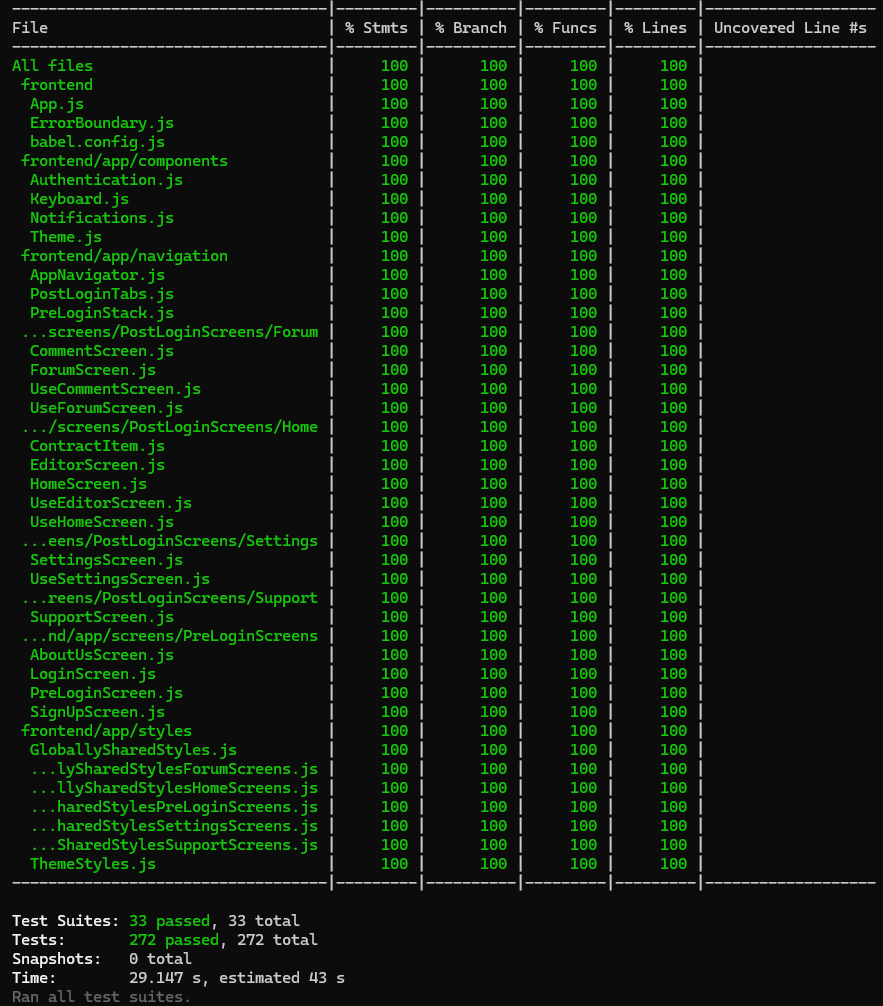
\includegraphics[width=1\textwidth]{LATEX/Appendices/Images/Software/Frontend/frontend_testing_report.png}
    \caption{Frontend Test Coverage Report}
    \label{fig:frontend_testing}
\end{figure}

\section{CI/CD Pipeline}

\subsection{Continuous Integration}

Through Continuous Integration, tests get automatically executed on a regular basis, which in turn improves software quality. The support for this feature was added for the backend and frontend codebases using \texttt{GitHub Actions}. The \texttt{CI/CD} pipeline is defined in the \textit{.github/workflows} directory, which is triggered anytime a push or pull request is made to the main branch. It is composed of several jobs, each responsible for a different part of the testing and deployment process. For the \textit{CI} part, it includes:

\begin{itemize}
    \item The pipeline uses the \textit{actions/checkout@v2} action to checkout the repository code to the runner.
    \item Python 3.11.2 is set up using \textit{actions/setup-python@v2}.
    \item Node.js 18.14.0 is set up using \textit{actions/setup-node@v2}.
    \item The pipeline installs necessary Python dependencies from the \textit{requirements.txt} file.
    \item The pipeline installs necessary npm dependencies for the frontend. The installation process includes the \textit{legacy-peer-deps} flag to tackle compatibility issues.
    \item The code is linted using \textit{flake8} to ensure code quality. This step includes checking for errors, warnings, and generating a report.
    \item Backend tests are run using \textit{pytest}.
    \item Frontend tests are executed using the \textit{npm run test} command.
\end{itemize}

\begin{figure}[!ht]
    \centering
    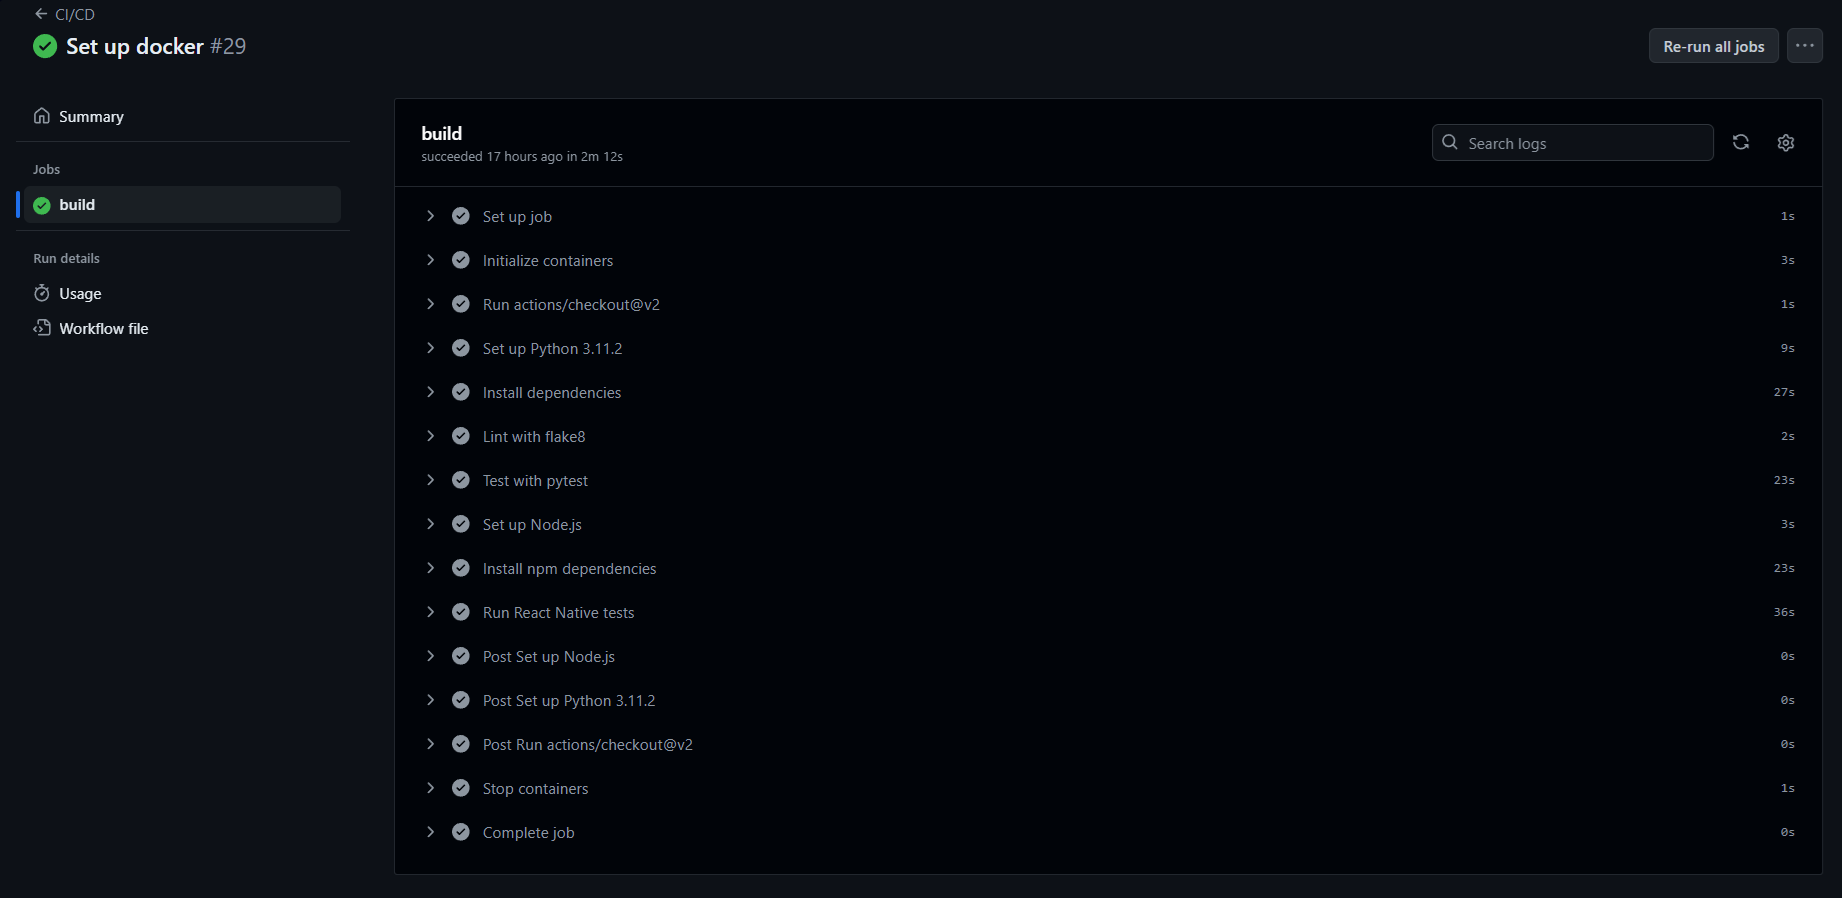
\includegraphics[width=1\linewidth]{LATEX/Appendices/Images/Pipeline_CI_CD/github_actions_CI_CD_pipeline.png}
    \caption{CI/CD Pipeline}
    \label{fig:CI/CD-Pipeline}
\end{figure}

\subsection{Continuous Deployment}

In the project, continuous deployment was implemented to automatically reflect any updates to the codebase in the production environment if all tests pass. The deployment process is hosted on \texttt{Google Cloud}, utilising a VM instance that accepts only HTTPS connections. This secure configuration protects the application during data transmission.

The project is containerised using \texttt{Docker}, allowing for consistent and fast deployment across different environments. The repository's structure reflects this, with \textit{Docker} configuration files for the \texttt{backend}, \texttt{frontend}, and \texttt{Nginx} server located in their respective directories. The main \textit{``docker-compose.yml''} file at the root of the repository handles the building and running of these services.

The server-side code resides in the \textit{``backend''} directory, which includes a \textit{``Dockerfile''} that sets up the \textit{Python} environment, installs dependencies, collects static files, runs database migrations, and starts the \textit{Daphne} server. The client-side code is located in the \textit{``frontend''} directory, where its respective \textit{``Dockerfile''} resides. It installs \textit{Node.js} dependencies, logs into \textit{Expo} using a token, and deploys the application to \texttt{Expo} servers. The \textit{nginx} directory contains the \textit{``Dockerfile''} and configuration for the respective server, which handles HTTPS termination and forwards requests to the backend. The setup also includes a \texttt{Redis} server, specified in the \textit{Docker} configuration, which is used for handling notifications. Additionally, \texttt{Certbot} is used to obtain \textit{SSL} certificates for the domain names acquired from \textit{Fasthosts}.

After the \textit{CI} pipeline jobs finish, if all tests pass, the pipeline proceeds to the \textit{CD} stage. During deployment, the pipeline connects to the VM instance, stops the currently running \textit{Docker} containers, pulls the latest code from the repository, and rebuilds the \textit{Docker} images using the \textit{``docker-compose up --build''} command. This process updates the backend and frontend services with the latest changes. The backend is deployed on the same VM instance, configured to accept requests from anywhere, while the frontend is deployed to the \textit{Expo} servers. Users can access the frontend application via a QR code or a link that forwards to the \textit{Expo} app, making it accessible from any location.

\section{Software Evaluation Strategy}

As the testing phase concludes, the evaluation methods employed for the software merit a discussion. The infrastructure, including both the backend and the frontend, was thoroughly unit tested, adhering to Weak Robust Equivalence Class based testing and obtaining a 100\% coverage across key parameters such as lines, functions, statements, and branches. Additionally, the frontend's UI/UX was tested by collecting user feedback from fellow students. Moreover, the software was also evaluated through CI/CD processes, ensuring that updates were efficiently integrated and deployed without disruptions. Furthermore, the AI model was tested using a validation dataset, with the training loss maintained below 0.001 and the validation loss below 0.01. The delegation of job performance metrics evaluation to the backend, which remains unimplemented, resulted in a reduction of the AI model's intended scope. Rather than integrating these metrics at the time of contract translation into code — a task that was found to be unfeasible — the AI model's functionality was adjusted. This adjustment led to the AI model translating contractual clauses into nearly identical code, differing only in variables such as USDC addresses of employers and employees, starting and ending dates, contract token interfaces, and other case-specific details. This code's execution depends on the data related to an employee's job performance, which was intended to be passed to the deployed contract by the backend, revealing that there was no necessity for the AI model as this could have been accomplished through simple parsing. However, despite these unexpected outcomes, the primary objective to provide an infrastructure for employment management was met, obviating the need for a precise evaluation of the AI model and smart contracts' behaviour.

\section{Limitations and Scope for Future Development}

\subsection{Unimplemented Features}

An essential component of the project that was disregarded consisted of the backend's ability to monitor and upload job performance metrics into smart contracts after their deployment. This feature was necessary in order to completely automate blockchain-based employment interactions, and without it, the software remains incomplete. Unfortunately, it was not implemented because of the project's large scope and strict time constraints. Although this is certainly possible, the approach to addressing this challenge would be substantially difficult. To fill this void, one could explore the possibility of deploying an AI system capable of dynamically writing scripts that adapt to various employers' CRM systems. However, implementing such a model might be difficult. Alternatively, the system could evolve into a startup platform, where smart contracts are built with the aid of the software implemented. In this case, developers would manually create scripts to extract data from CRM systems and feed it into smart contracts for each specific case.  

\subsection{Reflective Analysis on Smart Contract Deployment Strategy}

At the outset of this project, there was a significant gap in understanding how smart contract technology operates. It was initially believed that a new smart contract was required for each work interaction. Since deploying smart contracts involves substantial costs, creating a separate smart contract for every employment interaction proved economically unviable. A more strategic approach, which was realised later, would involve developing a single general smart contract to manage all employment interactions while creating separate instances of it for various employment scenarios. This approach would significantly reduce the cost and complexity of smart contract deployment.

\section{Comparison of Achievements and Requirements}

In the following analysis, the initial requirements will be compared with the accomplished achievements. The comparison is categorised into functional and non-functional requirements:

\subsection{Functional Requirements}

\begin{itemize}
    \item \textbf{Contract Conversion:} Achieved. The platform successfully converts traditional employment contracts into smart contracts using a fine-tuned \texttt{GPT-3.5 Turbo} model.
    \item \textbf{AI Model Integration:} Achieved. The AI model has been successfully integrated with the backend, allowing for efficient processing of contracts.
    \item \textbf{User Authentication:} Achieved. Secure user account creation and management have been implemented.
    \item \textbf{User Engagement:} Achieved. A forum for user interactions on topics related to the application's scope has been developed.
    \item \textbf{Contract Management:} Achieved. Users can create, view, update, and delete their smart contracts in the application.
    \item \textbf{Performance Metrics:} Not achieved. Automating the monitoring and uploading of job performance metrics into smart contracts was deemed too complex and, due to time constraints, was not implemented. %ELABORATE HERE%
    \item \textbf{Salary Management:} Achieved. The system handles salary payments using \textit{USDC Coin}.
    \item \textbf{Notifications:} Achieved. Users receive notifications regarding contract updates, forum interactions, and other relevant events.
    \item \textbf{Mobile Application:} Achieved. A user-friendly interface for both \textit{iOS} and \textit{Android} platforms has been developed.
    \item \textbf{Custom Theming:} Achieved. The UI supports both dark and light modes.
    \item \textbf{Admin Panel:} Achieved. An admin panel for managing users, contracts, and system settings has been implemented.
    \item \textbf{Dispute Resolution:} Partially achieved. The platform provides mechanisms for resolving disputes, but it relies on job performance metrics, which are not implemented.
\end{itemize}

\subsection{Non-Functional Requirements}

\begin{itemize}
    \item \textbf{Scalability:} Partially achieved. Although the system architecture was designed to handle an increasing number of users and contracts efficiently, no adequate load testing was performed; no horizontal scaling was applied; and load balancers were not employed due to tight time constraints.
    \item \textbf{Security:} Achieved. The platform incorporates security measures to protect user data. This includes encryption for data in transit using HTTPS, secure user authentication methods, and secure storage of sensitive data on user devices through the \textit{expo-secure-storage} library. Additionally, the use of smart contracts ensures tamper-proof transactions due to the nature of the technology.
    \item \textbf{Reliability:} Not achieved. Although the platform seems reliable for now, there was no use of redundant systems, regular backups, or failover mechanisms. Unfortunately, time constraints prevented the implementation of these features.
    \item \textbf{Performance:} Achieved. The system provides quick response times for user interactions, contract processing, and AI model predictions. Thorough optimisation was applied during each sprint cycle to enhance the efficiency of all algorithms and code. Moreover, the software was designed to avoid heavy computations, with the exception of document translation into \textit{Solidity} code, which is executed on \textit{OpenAI's} servers.
    \item \textbf{Usability:} Achieved. The mobile application interface is intuitive, providing a positive user experience. User feedback was collected from peer students and incorporated during the development process to improve usability. In addition, the application supports both \textit{iOS} and \textit{Android} platforms.
    \item \textbf{Compliance:} Achieved. The platform complies with relevant regulations regarding employment contracts and data protection, such as GDPR. This was achieved through data anonymisation techniques, obtaining user consent for data usage, and ensuring that all data processing activities are compliant with legal standards.
    \item \textbf{Maintainability:} Achieved. The codebase is modular, allowing for easy updates and maintenance. It is well-documented with \textit{README.md} files and inline comments explaining each class or function written, and the code itself is self-explanatory most of the time.
    \item \textbf{Portability:} Achieved. Containerisation technique was applied with the aid of \textit{Docker} to package the application and its dependencies. This makes it easy to migrate the system to different cloud providers or on-premises servers if needed.
\end{itemize}

In conclusion, despite some unimplemented features and partial achievements, the project successfully met the vast majority of its initial requirements and objectives, laying a foundation for future development.

\section{Learning Outcomes}

This project, which totaled over 20,000 lines of self-written code (excluding package locks, migrations, static files, and other auto-generated files), provided a solid learning experience, highlighting the importance of several industry best practices in software development. Some of the key lessons learnt include:

\paragraph{Adherence to Test-Driven Development}

The primary lesson learned is the importance of adhering to Test-Driven Development (TDD). According to Boehm's curve, as software development proceeds, the cost of repairing bugs rises considerably. If TDD had been implemented from the outset, potential disruptions could have been mitigated early on. This might have even allowed for the correction of issues in the smart contract deployment strategy. Another significant learning point related to TDD adherence is the realisation that testing should not be left until the last moment, as it reveals critical bugs. More importantly, testing often proves more challenging than writing the original code, requiring three to five times more lines of code. Concluding, TDD allows for the clear definition of expected code behaviour, helping to maintain an architecture that is resistant to unnecessary future changes resulting from defects.

\paragraph{Continuous Integration and Continuous Deployment Practices}

Implementing a CI/CD pipeline is a must-have practice. It helps in maintaining a high standard of code quality through automated tests \& deployment and, more importantly, in identifying issues as development progresses. 

\paragraph{Clear Definition of Requirements}

Another major takeaway from this project is that specific needs must be carefully defined before any development begins. Unclear requirements can lead to unnecessary project expansions, delays, and resource wastage.  In order to align the project's aims with the expected outcomes, all stakeholders must engage in thorough requirement gathering and validation.

\paragraph{Progress Tracking with Project Management Tools}

\texttt{Trello} and other project management tools have proven extremely effective for tracking progress and meeting deadlines. These tools provide clarity and accountability for the developers, assisting them in identifying bottlenecks early. Furthermore, an agile project management approach helps the development team react more readily to changes by encouraging regular feedback.

\paragraph{Iterative and Incremental Development}

Applying an iterative and incremental development approach is helpful. This technique enables scheduled releases with precise goals, allowing the team to test and refine the system by breaking it down into smaller components. Additionally, frequent demonstrations of progress help maintain stakeholder interest.

\paragraph{Documentation and Code Reviews}

The development process should involve detailed documentation and periodic code reviews. This is needed in order to ensure that the system is maintainable not only by the original developers, but also future team members. Additionally, regular code reviews also help preserve adherence to best software engineering principles, which in turn allows for easy knowledge sharing across the team.

\paragraph{User-Centred Design Focus}

Even though this was not incorporated in the project, it was later realised that maintaining a focus on user-centred design is crucial. Gathering feedback from users during the design phase allows the product to meet their expectations. Moreover, engaging users is essential for the project's financial success.

\paragraph{Risk Management and Mitigation Strategies}

Finally, proactive risk management should be an ongoing practice. Risk mitigation strategies should be developed for all potential risks identified at the outset and throughout the project's implementation. This involves regular risk assessment meetings and updating the risk matrix to address new challenges as they arise. 

\paragraph{Errors in Popular Frameworks}

Not all highly used frameworks are error-free. Given the complexities of modern software, even widely adopted frameworks contain errors and buggy code. For example, one issue encountered was related to React Native. During development, the UI was constantly returning the warning: "Animation Warning - Sending onAnimatedValueUpdate with no listeners registered." After extensive research, it was revealed that this well-known issue, related to the conditional rendering of screens in navigation, remains unresolved despite extensive documentation and community awareness \cite{GithubAnimatedViewWarning, StackOverFlowAnimatedViewWarning}. While \textit{React Native} is a powerful framework for building cross-platform applications, the use of \textit{JavaScript} introduces challenges due to its non-strict typing, which can cause numerous errors. In future projects, it would be beneficial to consider using \textit{TypeScript} to mitigate these issues.

\paragraph{Limitations of Django Rest Framework}

While the \textit{Django Rest Framework} (DRF) is highly effective for creating robust APIs, it is not the fastest client-server framework. \textit{Python}, being an interpreted language rather than a compiled one, introduces performance limitations. Additionally, DRF can sometimes struggle with high concurrency scenarios compared to frameworks built with more performant languages like \textit{Go} or \textit{Node.js}. For future projects requiring high performance, it might be worth considering these alternatives.

\paragraph{Conclusion}

This project has demonstrated the significance of structured and disciplined software development processes. Each lesson learnt contributes to more efficient project management and execution in future software development projects.

\chapter{Conclusion}

\section{Achievements and Conclusions}

The project has succeeded in achieving the following accomplishments:

\begin{enumerate}
    \item An AI model was fine-tuned to translate legal employment contracts into smart ones for autonomous execution on the blockchain.
    \item A backend API was established to manage interactions with the AI model and support additional functionalities such as user management, forum communications, convenient editors and means to interact with the platform.
    \item A practical mobile application was developed with an intuitive UI/UX design.
    \item Together with a successful CI/CD pipeline integration, 100\% test coverage was attained for the backend, frontend, and AI component.
    \item The system with preliminary functionalities was deployed, being ready for the initial alpha/beta testing phases.
\end{enumerate}

Apart form the implementation achievements, this dissertation has attracted the interest of investors from \texttt{Block Dojo}, a global venture builder. Their investment has highlighted the project's potential, while also marking the start of the next round of software development based on the dissertation's findings. \textit{Block Dojo} has acquired a 10\% equity in the project, offering significant financial and strategic support for its growth. Furthermore, \texttt{IBM} has been the main stakeholder in this research. Their assistance has helped in assuring compliance with industry norms and expectations. Recognising the original quality of the research, an invitation was made to present it at the annual King's College London \texttt{Research Showcase Conference}. Being one of only two undergraduate students selected for this event, the findings and implications of the work were shared with a broader academic and professional audience.

One of the main goals of this thesis was to study the applications of artificial intelligence and smart contracts to understand their potential in solving the problem of mutual trust on the web. Through the development and implementation process, the study sought to advance personal knowledge of these technologies and identify potential markets that could significantly benefit from their application.

The study showed that it is difficult to fully automate employment interactions using smart contracts. While the technology itself shows great potential, real-world automation is challenging to achieve due to factors such as market preparedness, regulatory compliance, and technological constraints. Although the current implementation is not yet ready for widespread production use, it has laid a solid foundation for further development. Moreover, the underlying technologies themselves have demonstrated enormous promise in a variety of sectors. Subsequent development in industries such as real estate and marketing could yield significant economic and operational efficiencies. It will likely involve advancing the technology and enhancing its security protocols.

\section{Future Directions of the Research}

Upon conducting the research, one potential monetisable field was discovered. In the conventional process, small businesses engage with influencers to market their products through direct negotiations over the web, agreeing on terms and settling payments upfront without signing any legal documents to hold parties liable. This process is rife with scams, where either advertisers pay for services that they do not receive, or influencers go unpaid after completing promotional work. Therefore, moving forward to a Master's degree, there is an option to continue this research by applying the technology to the more feasible field discussed above. The proposed solution involves:

\begin{itemize}
    \item Creating a platform where users can directly track their marketing offers, monitor their fulfilment, and make new offers. This platform would integrate with social media APIs, providing an overview of influencers' account statistics, including their average views, likes, comments per post, user engagement, and all other relevant information.
    \item Advertisers deposit payment into a smart contract.
    \item \textbf{Three-Part Authentication for Payment Release:} The smart contract designed for these transactions would require three signatures to release funds:
    \begin{enumerate}
        \item From the brand ambassador, confirming agreement to the terms.
        \item From the advertiser, who tops up the smart contract.
        \item From the backend system, which validates the completion of the advertisement criteria as stipulated in the contract.
    \end{enumerate}
    \item \textbf{Automated Verification via AI:} Upon notification from the influencer that the promotional content has been posted, the platform's backend retrieves the data and passes it to a fine-tuned AI model that analyses the content to ensure it meets all agreed-upon promotional standards and criteria. 
    \item \textbf{Secure Funds Transfer:} Once the AI system confirms that all conditions have been met, the smart contract automatically processes the payment.
    \item \textbf{Why this Software is Realisable:} With the original topic of the dissertation, a significant challenge was the verification of dynamic data, which is complex to compute and not universally available from all companies. On the contrary, with this software, the data can be easily tracked since all social media (SM) content, whether posts, stories, or videos, can be pulled from the APIs of these SM platforms and verified against the agreed conditions of the offer. For instance, it can easily be ensured that a post highlights the product positively and mentions its specific features through modern Large Language Models, which can efficiently perform this verification through their advanced contextual awareness.
\end{itemize}

In light of the feasibility and promising potential of this application, it has been decided in collaboration with \textit{Block Dojo} to proceed with the development of this platform for marketing as the primary focus for the next phase of research and development.

Alternatively, if progressing directly to a PhD, this research could be continued in its original topic, attempting to tackle the issue of automated job performance metrics tracking and evaluation.


%%%%%%%%%%%%%%%%%%%%%%%%%%%%%%%%%
% References
%%%%%%%%%%%%%%%%%%%%%%%%%%%%%%%%%
\bibliographystyle{plain}
\bibliography{references}
\addcontentsline{toc}{section}{Bibliography}

%%%%%%%%%%%%%%%%%%%%%%%%%%%%%%%%%
% Appendices
%%%%%%%%%%%%%%%%%%%%%%%%%%%%%%%%%
\appendix
\include{Appendices/appendix}
\chapter{User Guide}
\section{Instructions}
You must provide an adequate user guide for your software. The guide should provide easily understood instructions on how to use your software. A particularly useful approach is to treat the user guide as a walk-through of a typical session, or set of sessions, which collectively display all of the features of your package. Technical details of how the package works are rarely required. Keep the guide concise and simple. The extensive use of diagrams, illustrating the package in action, can often be particularly helpful. The user guide is sometimes included as a chapter in the main body of the report, but is often better included in an appendix to the main report.

\chapter{Source Code}

The diagram below represents a structured listing of files and directories involved in the project. It visualises the organisation and hierarchy of the project's components as follows:
\begin{itemize}
    \item \textbf{Rounded Rectangles:} These shapes indicate directories, which are containers that hold files or other directories.
    \item \textbf{Regular Rectangles:} These represent code files within the directories.
    \item \textbf{Connecting Lines:} The lines show the hierarchical relationships between directories and files. If a line connects one rectangle or rounded rectangle to another, it indicates that the item at the arrow's end is contained within the item from which the line originates.
    \item \textbf{Colour Coding:} The colour of each figure signifies its level in the hierarchy. For instance, directories like \textit{backend}, \textit{frontend}, \textit{nginx}, and \textit{AI-models} are all coloured green, indicating they are at the same hierarchical level.
\end{itemize}

The image is high resolution; please enlarge it by pressing \textit{Ctrl} and scrolling up with the mouse to read it clearly.

\begin{figure}
    \centering
    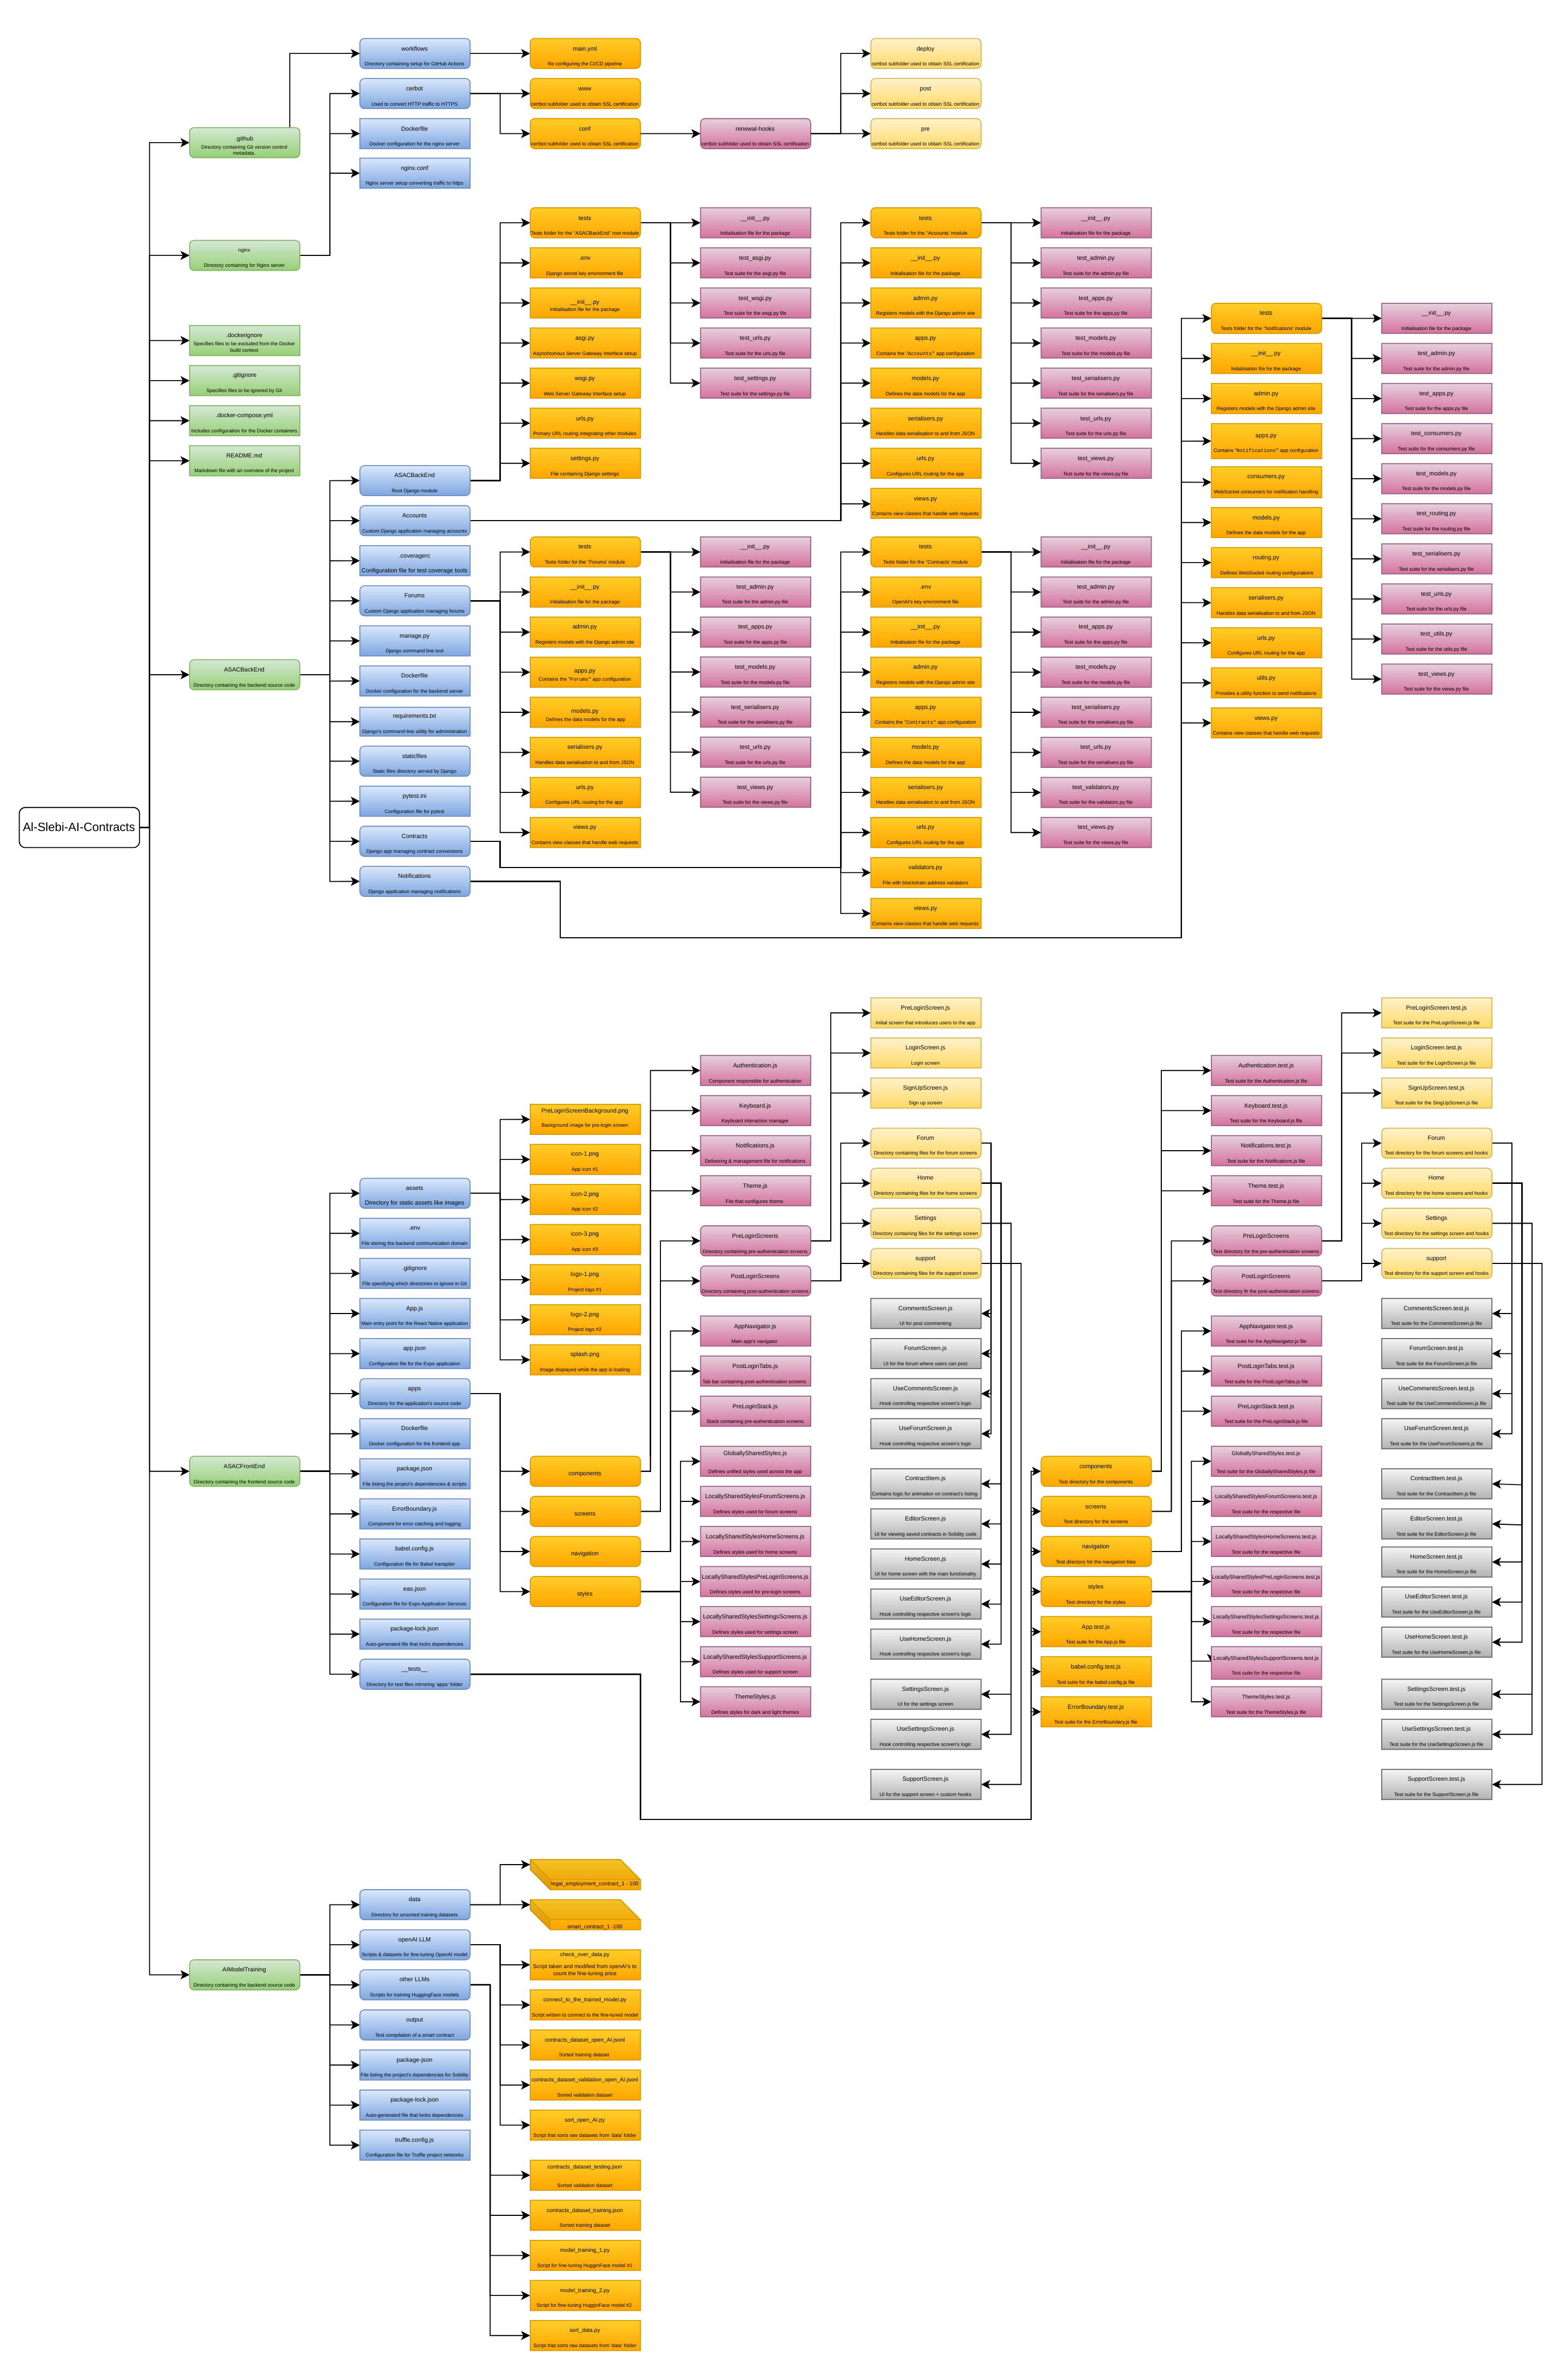
\includegraphics[width=1\linewidth]{LATEX/Appendices/Images/Software/files-listing.png}
    \label{fig:files-listing}
\end{figure}
\end{document}
